\documentclass[a4paper,titlepage,12pt]{scrartcl}	%El modo de documento es para la numeración.

\usepackage{graphicx} %Imágenes
\usepackage[utf8]{inputenc} %Tildes
\usepackage[spanish,es-tabla]{babel} %Español, es-table: llamar tablas en vez de cuadros
\usepackage[breaklinks=true]{hyperref} %Hiperenlaces
\usepackage{amssymb, amsmath, amsbsy} %Símbolos matemáticos
\usepackage{float} %Mover las imágenes usando [H]
\usepackage{eurosym} %Símbolo de euro \euro
\usepackage{listings} %Código

\numberwithin{figure}{section} %Hace que la primera figura de cada sección X sea X.1
\numberwithin{table}{section} %Hace que la primera tabla de cada sección X sea X.1

\begin{document}
	\begin{titlepage}
		\begin{center}
			\begin{figure}[htb]
				\begin{center}
					
\includegraphics[width=12cm]{./Portada/ugr.png}
				\end{center}
			\end{figure}

			\vspace*{0.8cm}
			\begin{Large}
				\textbf{Grado en Ingeniería Informática.}\\
			\end{Large}
			\begin{Huge}
				\vspace{1.5cm}
				\textbf{Práctica 3.} \\
			\end{Huge}
			\vspace*{0.76cm}
			\rule{100mm}{0.1mm}\\
			\vspace*{0.5cm}
			\begin{large}
				\textbf{Nombre de la asignatura:}\\
				Ingeniería de Servidores.\\
				\vspace*{0.5cm}
				\textbf{Realizado por:}\\
				Néstor Rodríguez Vico \\

				\vspace*{2cm}
				\begin{figure}[htb]
					\begin{center}
						
\includegraphics[width=5cm]{./Portada/etsiit.png}
					\end{center}
				\end{figure}
				\vspace*{-0.6cm}
				ESCUELA TÉCNICA SUPERIOR DE INGENIERÍAS INFORMÁTICA Y DE TELECOMUNICACIÓN.\\
				\rule{20mm}{0.1mm}\\
				\vspace*{0.6cm}
				Granada, \today.
			\end{large}
		\end{center}
	\end{titlepage}
	
	%--------------Indices--------------
	\tableofcontents
	\clearpage
	\listoffigures %Imagenes
	\clearpage
	%----------------------------------
	
	%%%%%%%%%%%%%%%%%%%%%%%%%%%%%%%%%%%%%%%%%%%%%%%%%%%%
	%%%%%%%%%%%%%%%%%%%% Cuestión 1 %%%%%%%%%%%%%%%%%%%%
	%%%%%%%%%%%%%%%%%%%%%%%%%%%%%%%%%%%%%%%%%%%%%%%%%%%%	
	\section[Cuestión 1:]{Cuestión 1:}
	\subsection[a) ¿Qué archivo le permite ver qué programas se han	instalado con el gestor de paquetes?]{a) ¿Qué archivo le permite ver qué programas se han	instalado con el gestor de paquetes?}
	
	Como podemos ver en la página de Ubuntu \cite{apthistory} el archivo que contiene dicha información en Ubuntu Server es \textit{/var/log/apt/history.log}. En CentOS se encuentra en la misma ruta. El archivo es \textit{/var/log/yum.log}. El contenido de dichos archivos se puede ver en la figura \ref{1-install_log}.
	
	\begin{figure}[H]
		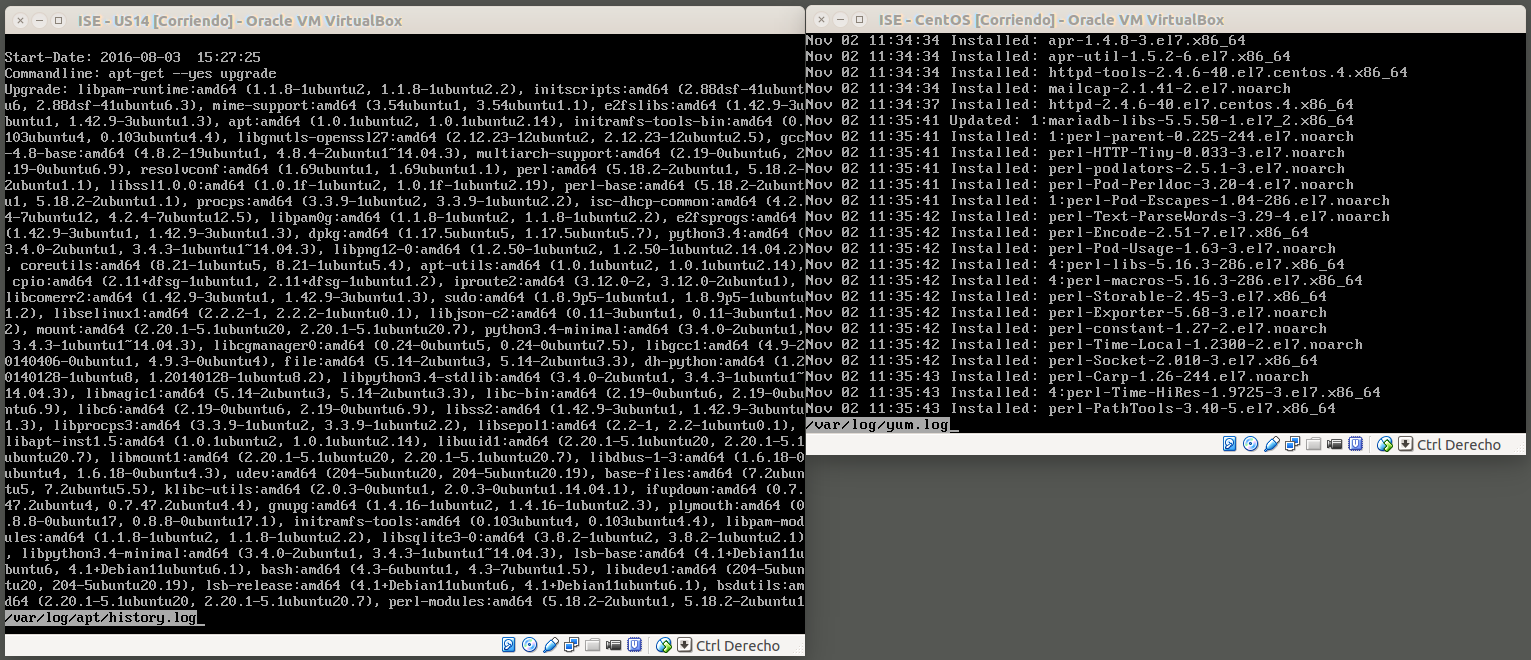
\includegraphics[width=\linewidth]{./Imagenes/1-install_log.png}
		\vspace{-0.5cm}
		\caption[A la izquierda el contenido de \textit{/var/log/apt/history.log} en Ubuntu Server. A la derecha el contenido de \textit{/var/log/yum.log} en CentOS.]{A la izquierda el contenido de \textit{/var/log/apt/history.log} en Ubuntu Server. A la derecha el contenido de \textit{/var/log/yum.log} en CentOS.}
		\label{1-install_log}
	\end{figure}
	
	\subsection[b) ¿Qué significan las terminaciones .1.gz o .2.gz de los archivos en ese directorio?]{b) ¿Qué significan las terminaciones .1.gz o .2.gz de los archivos en ese directorio?}
	
	En mi caso existen dichos archivos en el directorio\textit{/var/log}, como podemos ver en la imagen \ref{1-archivos_gz}. Dichos archivos son creados con el comando \textit{logrotate} \cite{logrotate} de forma periódica, para comprimir los \textit{logs} y que el fichero \textit{log} no crezca demasiado.
	
	\begin{figure}[H]
		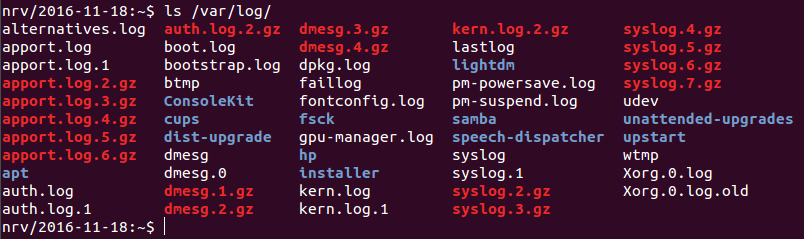
\includegraphics[width=\linewidth]{./Imagenes/1-archivos_gz.png}
		\vspace{-0.5cm}
		\caption[Contenido del directorio \textit{/var/log/} en mi máquina anfitirona.]{Contenido del directorio \textit{/var/log/} en mi máquina anfitirona.}
		\label{1-archivos_gz}
	\end{figure}

	%%%%%%%%%%%%%%%%%%%%%%%%%%%%%%%%%%%%%%%%%%%%%%%%%%%%
	%%%%%%%%%%%%%%%%%%%% Cuestión 2 %%%%%%%%%%%%%%%%%%%%
	%%%%%%%%%%%%%%%%%%%%%%%%%%%%%%%%%%%%%%%%%%%%%%%%%%%%
	\section[Cuestión 2: ¿qué archivo ha de modificar para programar una tarea? Escriba la línea necesaria para ejecutar una vez al día una copia del directorio ~/codigo a ~/seguridad/\$fecha donde \$fecha es la fecha actual (puede usar el comando date).]{Cuestión 2: ¿qué archivo ha de modificar para programar una tarea? Escriba la línea necesaria para ejecutar una vez al día una copia del directorio ~/codigo a ~/seguridad/\$fecha donde \$fecha es la fecha actual (puede usar el comando date).}
	
	Cómo podemos ver en el manual de \textit{crontab} \cite{crontab} si queremos editar el archivo \textit{crontab} actual debemos ejecutar el comando \textit{crontab -e}, como podemos ver en la figura \ref{2-crontab-e}. En el caso de Ubuntu Server el fichero es \textit{/tmp/crontab.kWQ61Y/crontab}. En el caso de CentOS el fichero es \textit{/tmp/crontab.yxrpPw}.
	
	\begin{figure}[H]
		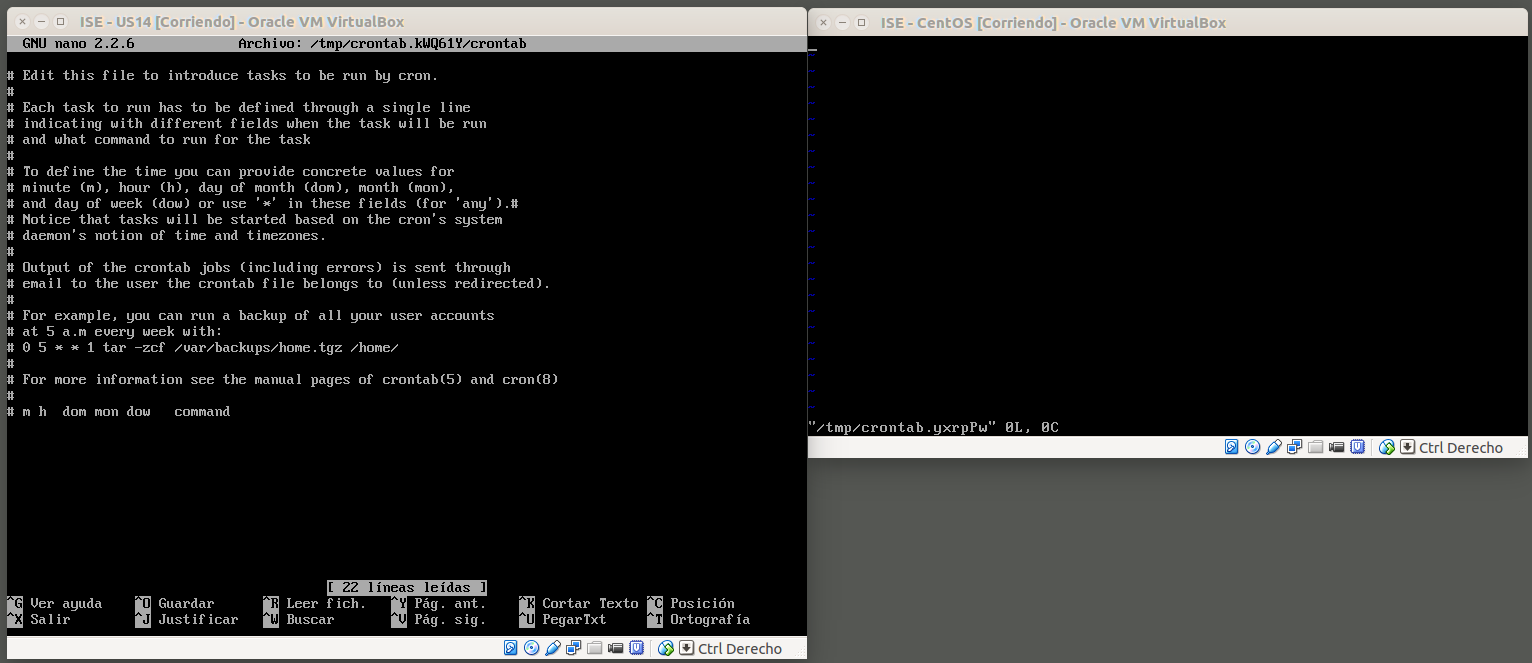
\includegraphics[width=\linewidth]{./Imagenes/2-crontab-e.png}
		\vspace{-0.5cm}
		\caption[Ejecución del comando \textit{crontab -e}; a la izquierda en Ubuntu Server y a la derecha en CentOS.]{Ejecución del comando \textit{crontab -e}; a la izquierda en Ubuntu Server y a la derecha en CentOS.}
		\label{2-crontab-e}
	\end{figure}

	Lo primero que he hecho ha sido crear el script \ref{scriptcrontab} y ubicarlo en el directorio \textit{$\sim$}, como se puede ver en la figura \ref{2-script}. Una vez tenemos todo listo, editamos el fichero \textit{crontab} añadiendo la línea \textit{00 11 * * * $\sim$/script.sh}, como se puede ver en el script \footnote{El script \textit{``2-scriptcrontab.sh''} se encuentra dentro de la carpeta \textit{Archivos auxiliares}.} \ref{scriptcrontab}. \\
	
	Script \ref{scriptcrontab}:
	\begin{lstlisting}[frame=single, basicstyle=\footnotesize, label={scriptcrontab}]
	#!/bin/bash
	
	fecha=$(date +"%m_%d_%Y")
	mkdir -p ~/seguridad
	mkdir -p ~/seguridad/$fecha
	cp -r ~/codigo ~/seguridad/$fecha
	\end{lstlisting}
	
	\begin{figure}[H]
		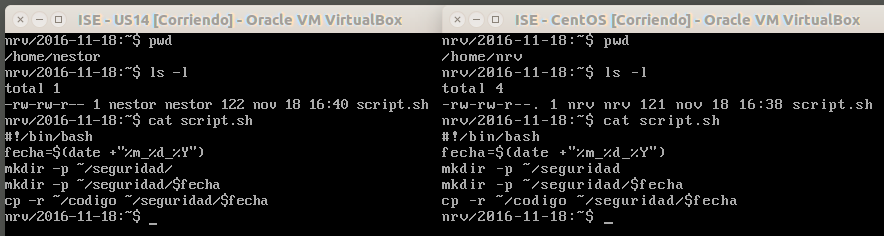
\includegraphics[width=\linewidth]{./Imagenes/2-script.png}
		\vspace{-0.5cm}
		\caption[Creación del script; a la izquierda en Ubuntu Server y a la derecha en CentOS.]{Creación del script; a la izquierda en Ubuntu Server y a la derecha en CentOS.}
		\label{2-script}
	\end{figure}
	
	\begin{figure}[H]
		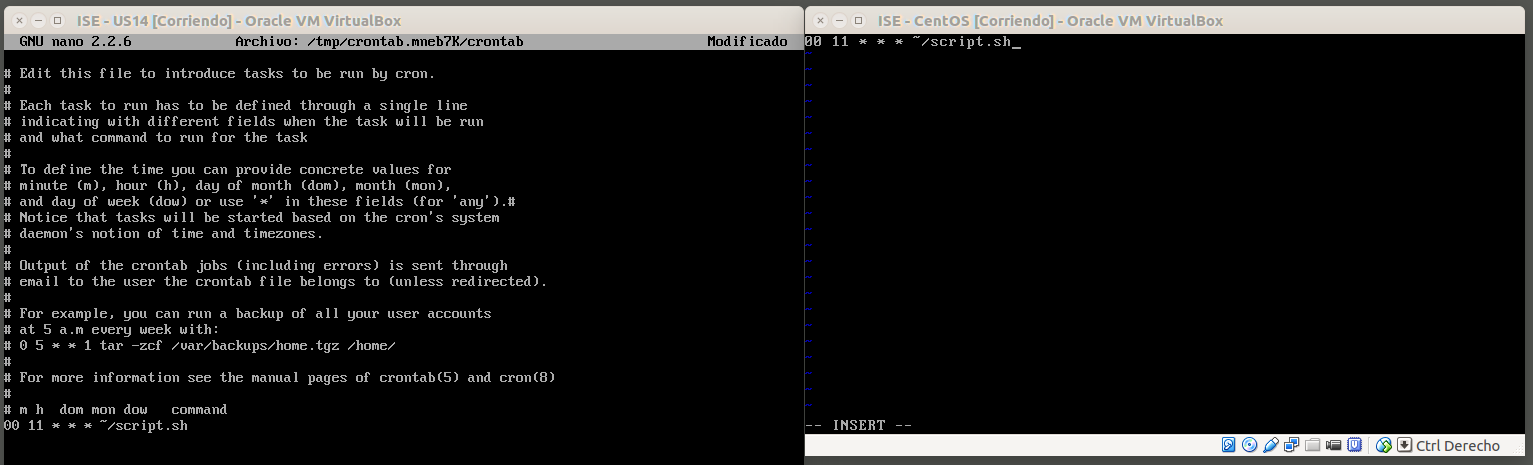
\includegraphics[width=\linewidth]{./Imagenes/2-crontab-mod.png}
		\vspace{-0.5cm}
		\caption[Fichero \textit{crontab} modificado; a la izquierda en Ubuntu Server y a la derecha en CentOS.]{Fichero \textit{crontab} modificado; a la izquierda en Ubuntu Server y a la derecha en CentOS.}
		\label{2-crontab-mod}
	\end{figure}
	
	%%%%%%%%%%%%%%%%%%%%%%%%%%%%%%%%%%%%%%%%%%%%%%%%%%%%
	%%%%%%%%%%%%%%%%%%%% Cuestión 3 %%%%%%%%%%%%%%%%%%%%
	%%%%%%%%%%%%%%%%%%%%%%%%%%%%%%%%%%%%%%%%%%%%%%%%%%%%
	\section[Cuestión 3: Pruebe a ejecutar el comando, conectar un dispositivo USB y vuelva a ejecutar el comando. Copie y pegue la salida del comando. (considere usar dmesg $\mid$ tail). Comente qué observa en la información mostrada.]{Cuestión 3: Pruebe a ejecutar el comando, conectar un dispositivo USB y vuelva a ejecutar el comando. Copie y pegue la salida del comando. (considere usar dmesg $\mid$ tail). Comente qué observa en la información mostrada.}
	
	El resultado de ejecutar \textit{dmesg $\mid$ tail} antes de conectar un USB es el que podemos ver en la figura \ref{3-antes}.
	
	\begin{figure}[H]
		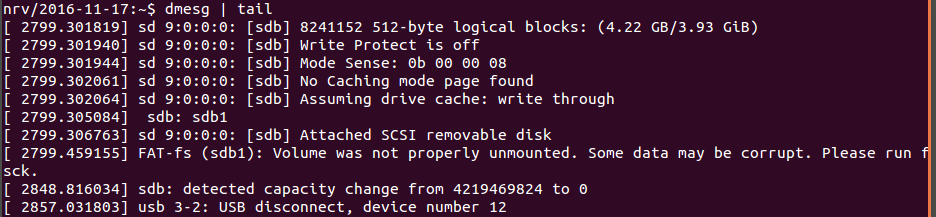
\includegraphics[width=\linewidth]{./Imagenes/3-antes.png}
		\vspace{-0.5cm}
		\caption[\textit{dmesg $\mid$ tail} antes de conectar el USB.]{\textit{dmesg $\mid$ tail} antes de conectar el USB.}
		\label{3-antes}
	\end{figure}
	
	El resultado de ejecutar \textit{dmesg $\mid$ tail} después de conectar un USB es el que podemos ver en la figura \ref{3-despues}.
	
	\begin{figure}[H]
		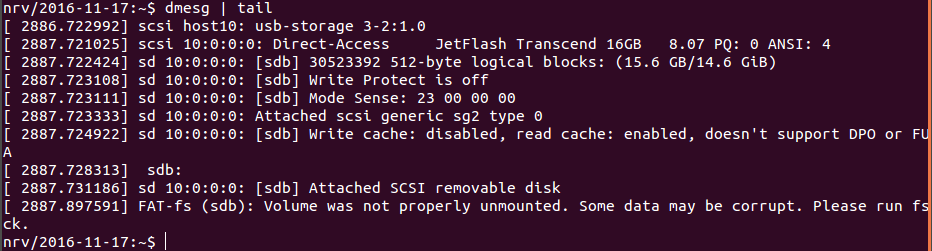
\includegraphics[width=\linewidth]{./Imagenes/3-despues.png}
		\vspace{-0.5cm}
		\caption[\textit{dmesg $\mid$ tail} después de conectar el USB.]{\textit{dmesg $\mid$ tail} después de conectar el USB.}
		\label{3-despues}
	\end{figure}
	
	En la salida tras conectar el almacenamiento USB podemos ver la siguiente información: 
	\begin{itemize}
		\item Línea 1: Se detecta el almacenamiento USB.
		\item Línea 2: Podemos ver el nombre del USB y su capacidad, 16GB.
		\item Línea 3: Vemos que hay 30523392 bloques lógicos de 512 byte cada uno. De los 15.6 GiB disponibles hay 14.6 GiB libres.
		\item Línea 4: La protección de escritura está desactivada, esto nos indica que se pueden escribir datos en el almacenamiento USB.
		\item Línea 7: La escritura en caché está desactivada y la lectura en caché activada.
		\item Línea 9: Es un almacenamiento USB que se puede remover.
		\item Línea 10: Mensaje que indica que no se desmontó correctamente y que algunos datos podrían estar corruptos.
	\end{itemize}
	
	%%%%%%%%%%%%%%%%%%%%%%%%%%%%%%%%%%%%%%%%%%%%%%%%%%%%
	%%%%%%%%%%%%%%%%%%%% Cuestión 4 %%%%%%%%%%%%%%%%%%%%
	%%%%%%%%%%%%%%%%%%%%%%%%%%%%%%%%%%%%%%%%%%%%%%%%%%%%
	\section[Cuestión 4: Ejecute el monitor de “System Performance” y muestre el resultado. Incluya capturas de pantalla comentando la información que aparece.]{Cuestión 4: Ejecute el monitor de “System Performance” y muestre el resultado. Incluya capturas de pantalla comentando la información que aparece.}
	
	Una vez terminado el análisis, nos aparece el informe con la información recogida. Podemos ver información de todo tipo, desde información sobre la CPU, la red, el disco o la memoria, como podemos ver en la figura \ref{4-resumen}.
	
	\begin{figure}[H]
		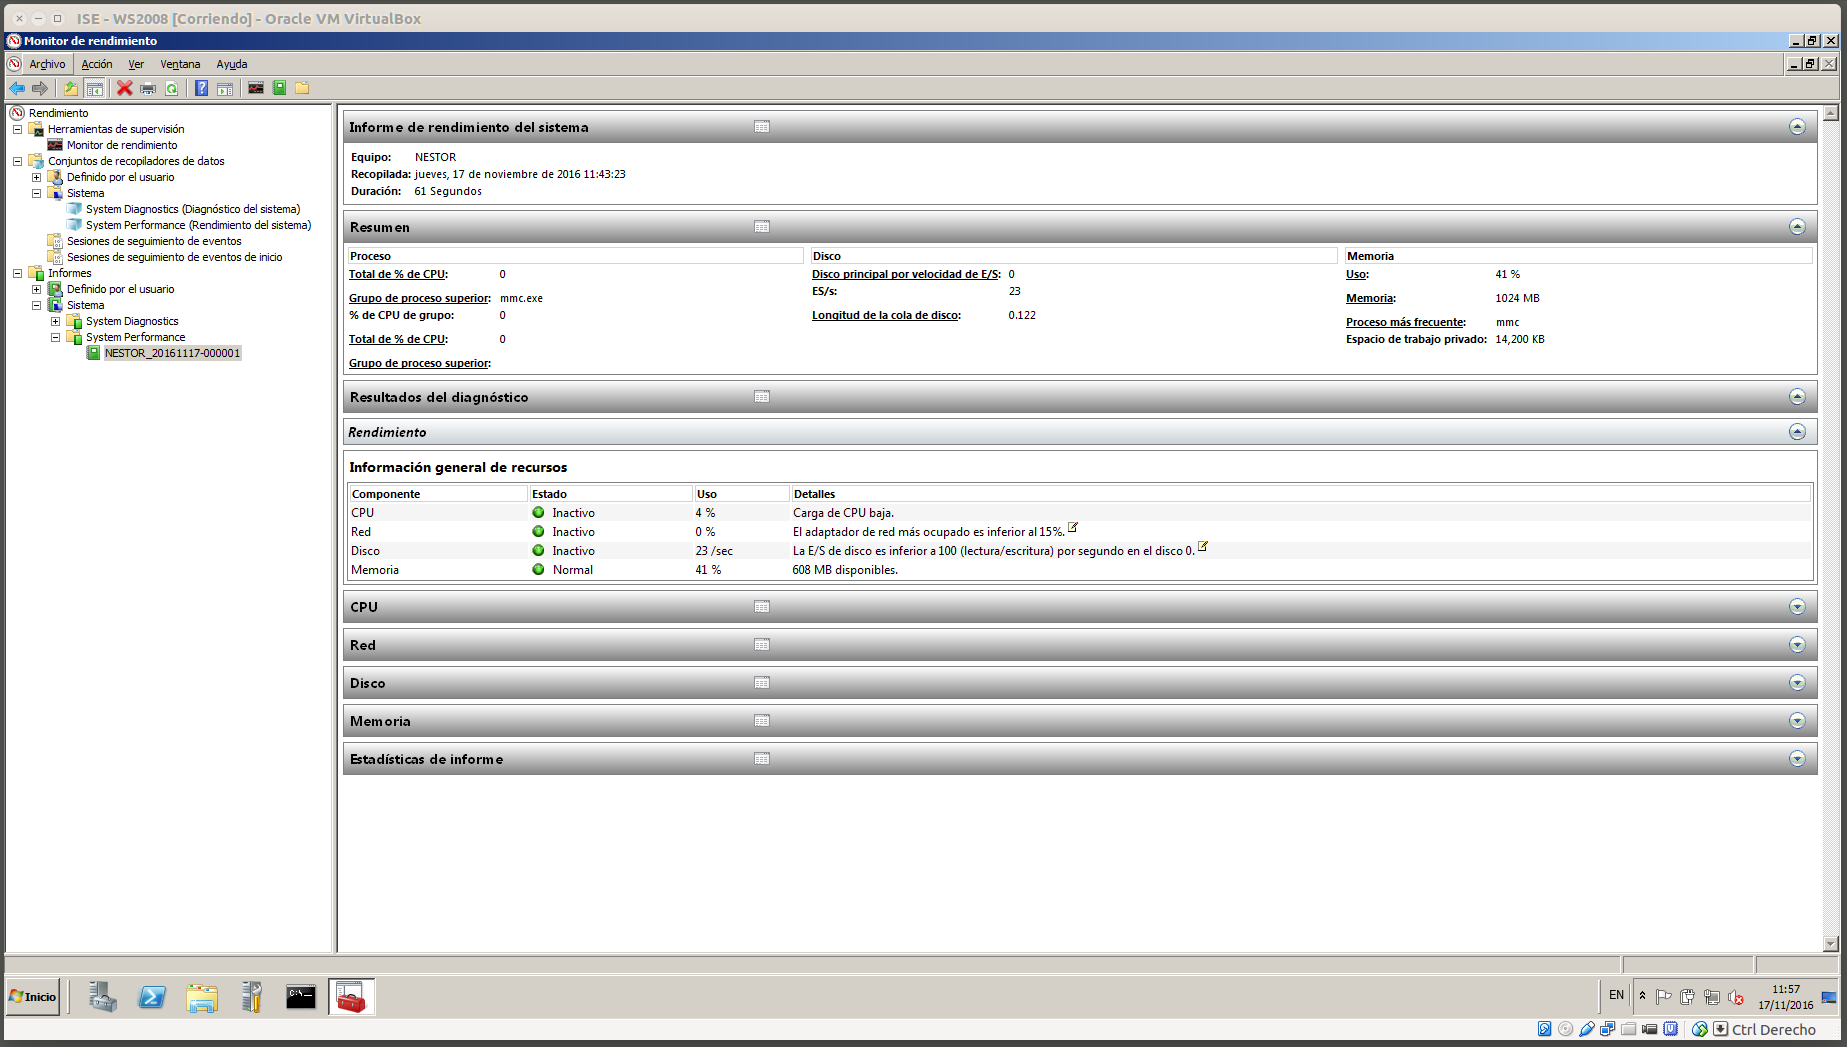
\includegraphics[width=\linewidth]{./Imagenes/4-resumen.png}
		\vspace{-0.5cm}
		\caption[Resumen del resultado del análisis.]{Resumen del resultado del análisis.}
		\label{4-resumen}
	\end{figure}
	
	El análisis nos aporta información de los campos que podemos ver en la figura \ref{4-categorias}:
	
	\begin{figure}[H]
		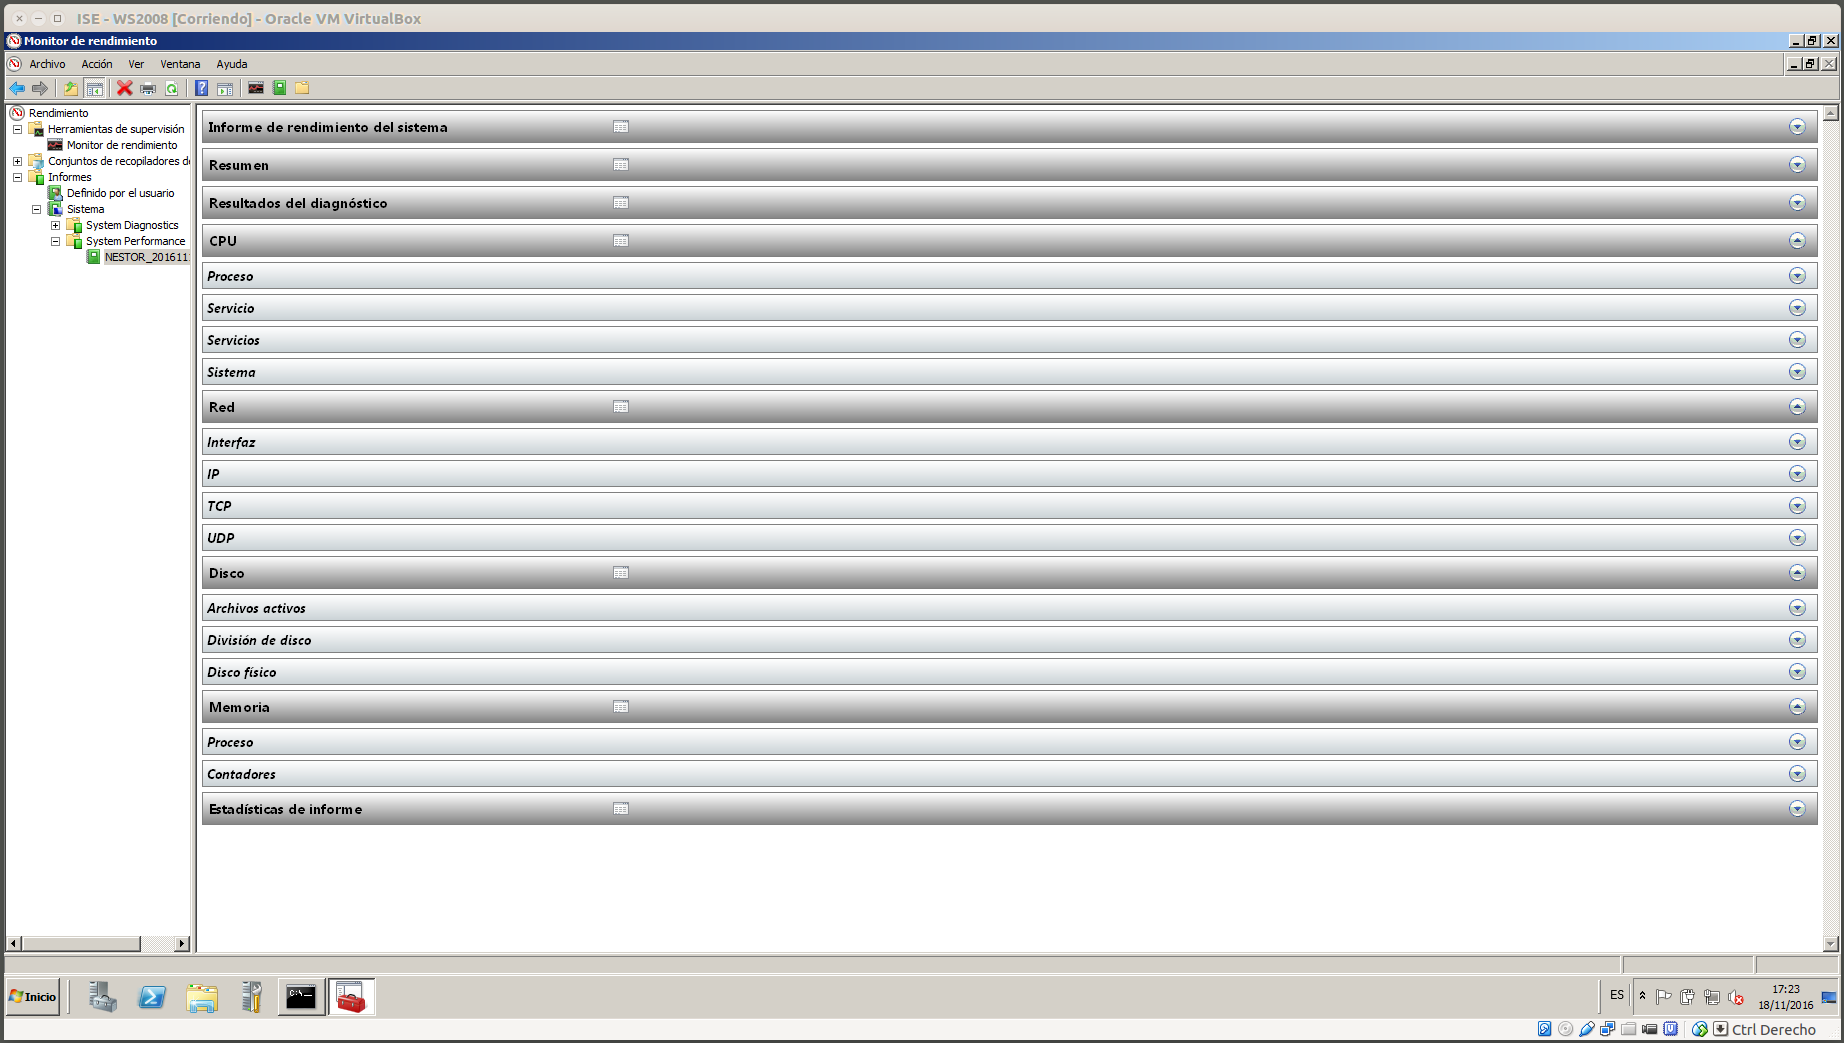
\includegraphics[width=\linewidth]{./Imagenes/4-categorias.png}
		\vspace{-0.5cm}
		\caption[Categorías de información del análisis.]{Categorías de información del análisis.}
		\label{4-categorias}
	\end{figure}
	
	Dentro de la categoría de los procesos podemos ver información sobre que procesos se han estado ejecutando durante el análisis e información sobre los mismos. Podemos ver que, por ejemplo, el proceso \textit{rundll32.exe} tiene el identificador de proceso 1152, ha iniciado 7 subprocesos, ha usado 3 subprocesos y ha ocupado un 0.1\% de CPU. También podemos ver información acerca del número de subprocesos o incluso el número de interrupciones que ha habido durante la ejecución del análisis. Todo esto y mucha más información lo podemos ver en la figura \ref{4-procesos}. \\
	
	Dentro de la categoría de los procesos podemos ver información sobre el uso de la memoria. Por ejemplo, podemos ver que durante el análisis se han producido de media 40 errores de páginas, ha habido de media 0.117 errores de caché y el número medio de páginas entradas libres en la tabla de páginas del sistema asciende a 33554694. Todo esto y mucha más información lo podemos ver en la figura \ref{4-memoria}.  \\
	
	\begin{figure}[H]
		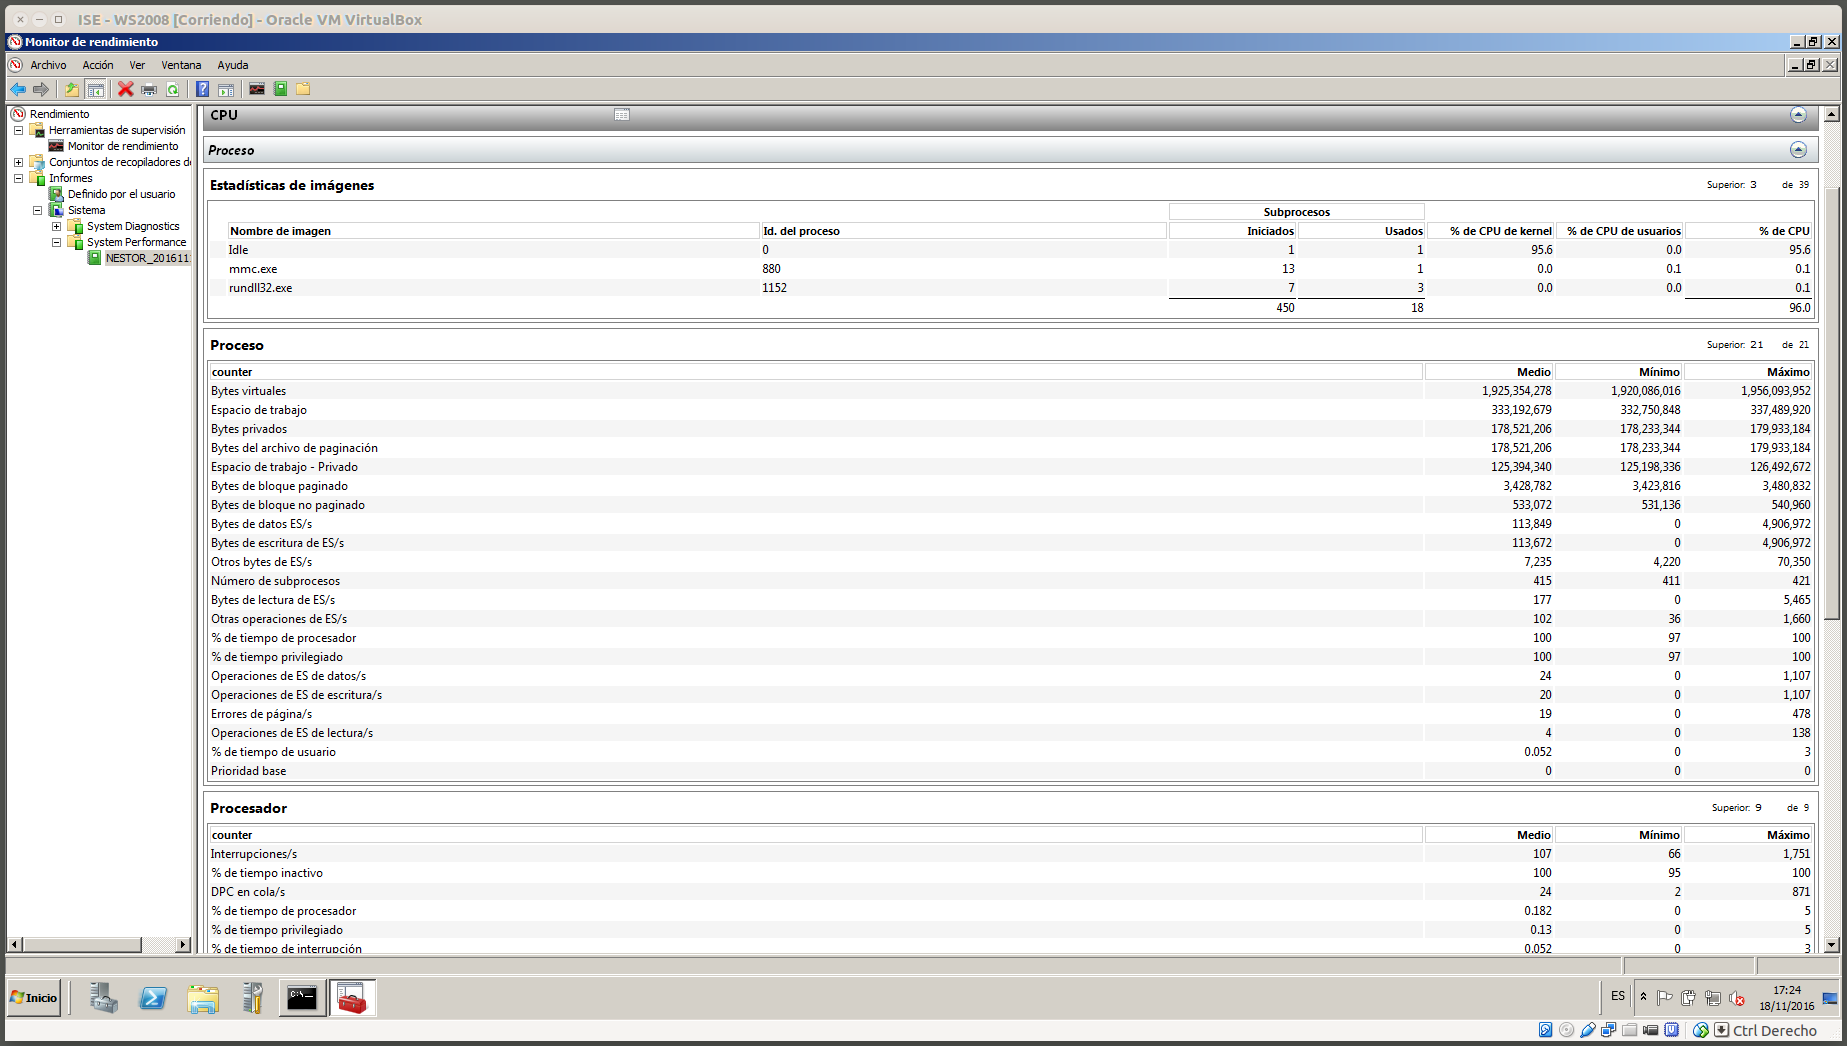
\includegraphics[width=\linewidth]{./Imagenes/4-procesos.png}
		\vspace{-0.5cm}
		\caption[Información acerca de los procesos.]{Información acerca de los procesos.}
		\label{4-procesos}
	\end{figure}
	
	\begin{figure}[H]
		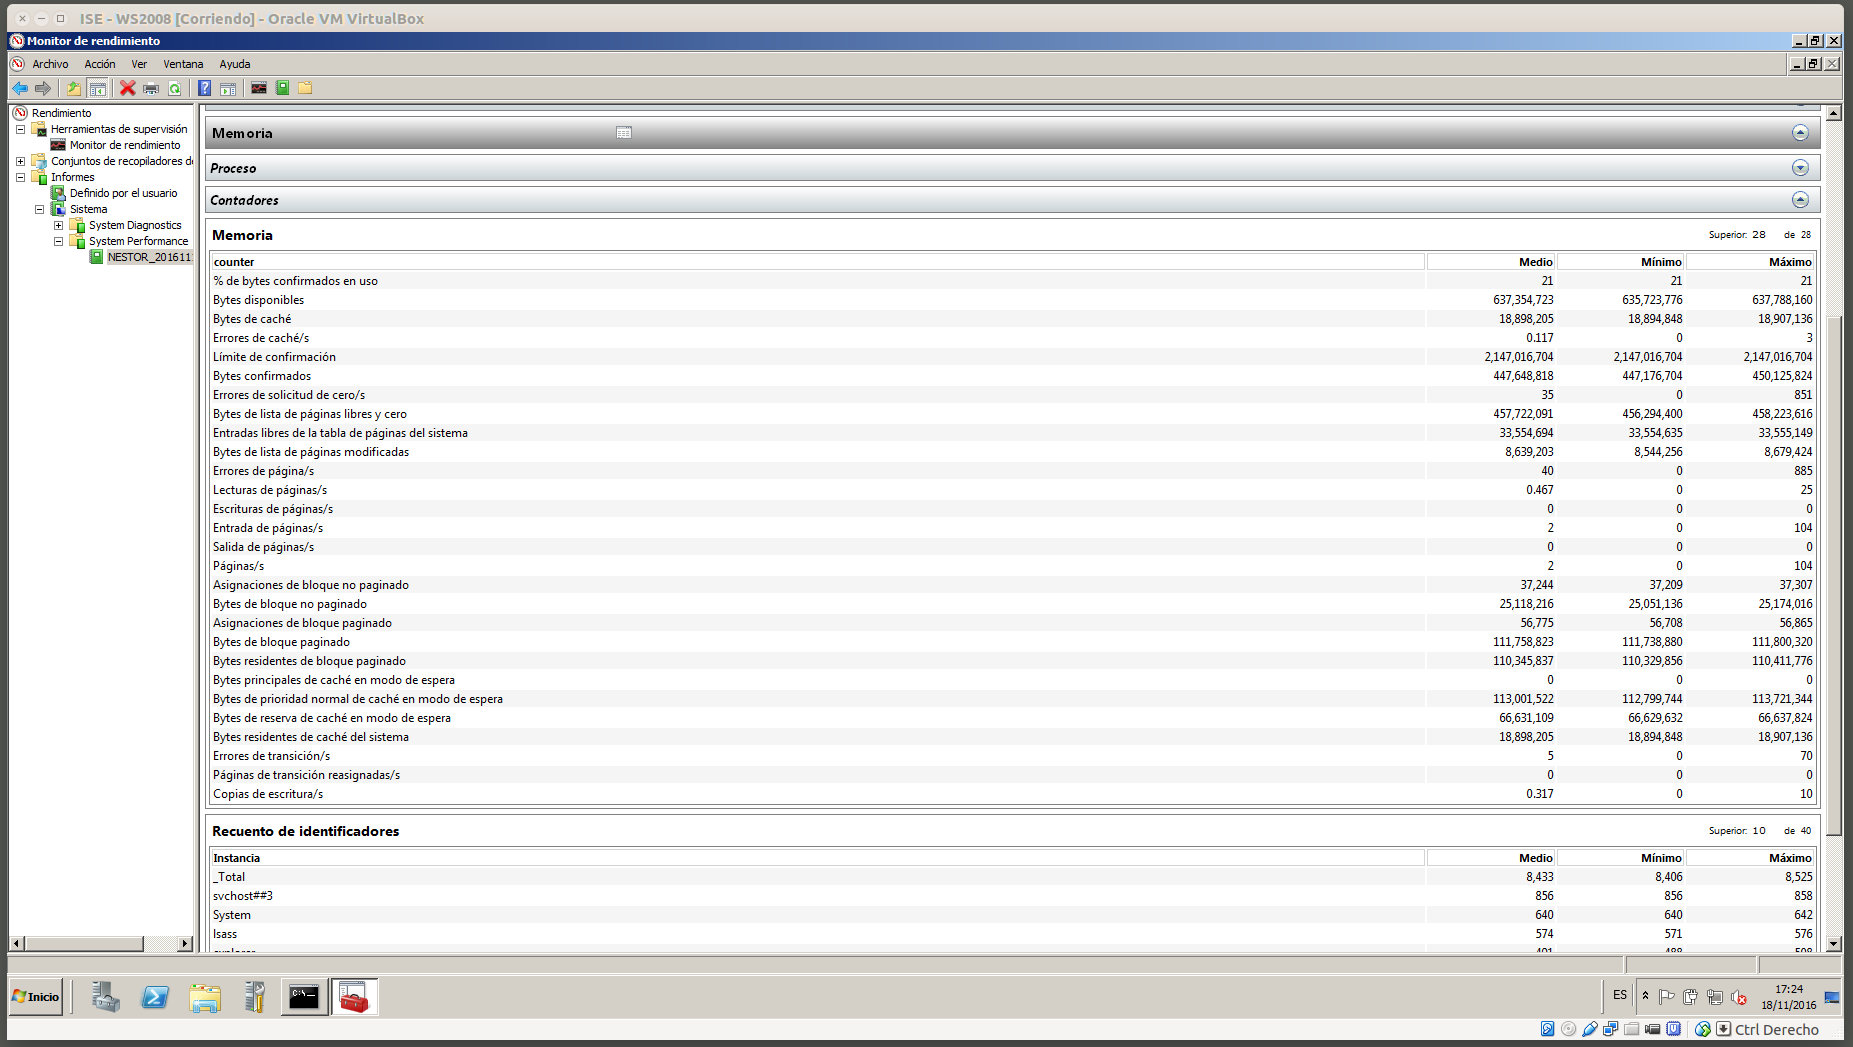
\includegraphics[width=\linewidth]{./Imagenes/4-memoria.png}
		\vspace{-0.5cm}
		\caption[Información acerca del uso de la memoria.]{Información acerca del uso de la memoria.}
		\label{4-memoria}
	\end{figure}
		
	%%%%%%%%%%%%%%%%%%%%%%%%%%%%%%%%%%%%%%%%%%%%%%%%%%%%
	%%%%%%%%%%%%%%%%%%%% Cuestión 5 %%%%%%%%%%%%%%%%%%%%
	%%%%%%%%%%%%%%%%%%%%%%%%%%%%%%%%%%%%%%%%%%%%%%%%%%%%
	\section[Cuestión 5: Cree un recopilador de datos definido por el usuario (modo avanzado) que incluya tanto el contador de rendimiento como los datos de seguimiento: Todos los referentes al procesador, al proceso y al servicio web. Intervalo de muestra 15 segundos. Almacene el resultado en el directorio Escritorio$\backslash$logs.]{Cuestión 5: Cree un recopilador de datos definido por el usuario (modo avanzado) que incluya tanto el contador de rendimiento como los datos de seguimiento: Todos los referentes al procesador, al proceso y al servicio web. Intervalo de muestra 15 segundos. Almacene el resultado en el directorio Escritorio $\backslash$logs.}
	
	\begin{enumerate}
		\item Nos posicionamos en la categoría de \textit{Definidos por el usuario} dentro de \textit{Conjuntos de recopiladores de datos} y le damos click derecho, a continuación a \textit{Nuevo} y finalmente a \textit{Conjunto de recopiladores de datos}, como podemos ver en la figura \ref{5-1}.
		\item Elegimos el nombre del recopilador. En mi caso he elegido \textit{RecopiladorISE}, como podemos ver en la figura \ref{5-2}.
		\item Elegimos que tipos de datos queremos recolectar. En mi caso \textit{Contador de rendimiento} y \textit{Datos de seguimiento de eventos}, como podemos ver en la figura \ref{5-3}.
		\item Ahora tenemos que seleccionar los datos que queremos recopilar. En un principio no hay ninguno seleccionado, como podemos ver en la figura \ref{5-4}.
		\item Para seleccionar los datos, nos vamos a la categoría que queremos y le damos al botón de agregar. En nuestro caso debemos agregar la categoría entera de \textit{procesador}, la de \textit{proceso} y la de \textit{servicio web}. El resultado final es el que podemos ver en la figura \ref{5-5}.
		\item Una vez hemos escogido los datos, seleccionamos el intervalo de muestra, en nuestro caso elegimos 15 segundos, como podemos ver en la figura \ref{5-6}.
		\item En los proveedores de seguimiento no seleccionamos nada, como podemos ver en la figura \ref{5-7}.
		\item A continuación elegimos donde queremos que se guarde la \textit{logs}, en nuestro caso queremos que se guarden en el la carpeta \textit{logs} dentro del \textit{Escritorio}, como podemos ver en la figura \ref{5-8}.
		\item Finalmente, seleccionamos la opción de iniciar el recopilador y le damos a finalizar, como podemos ver en la figura \ref{5-9}.
	\end{enumerate}
	
	\begin{figure}[H]
		\centering
		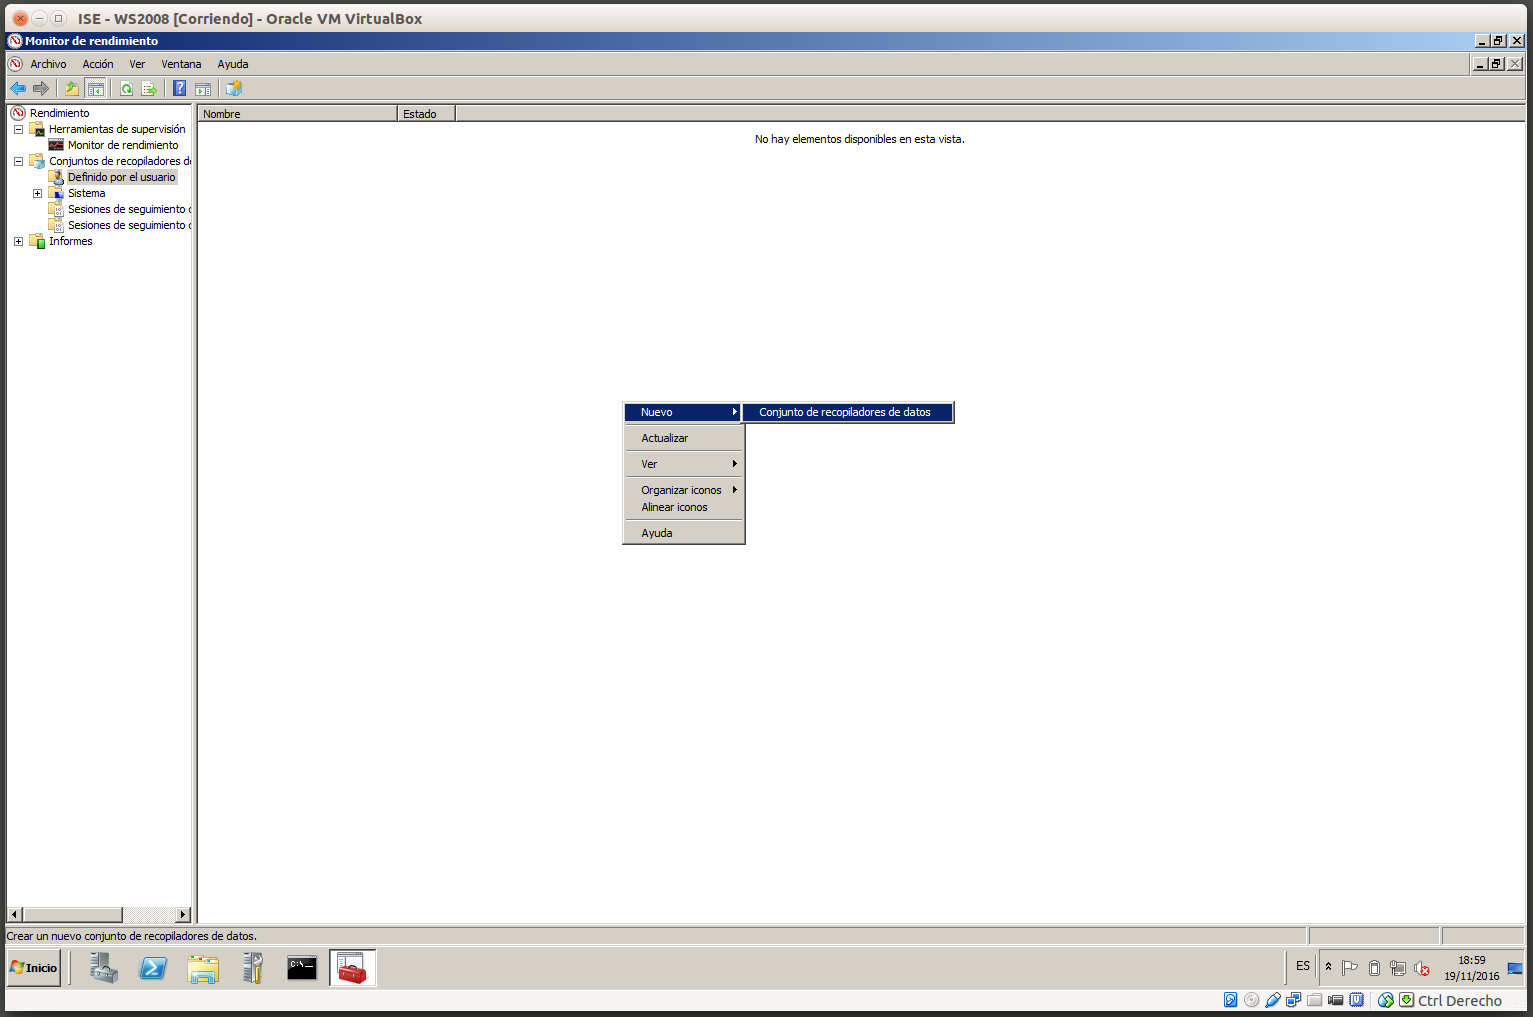
\includegraphics[scale=0.27]{./Imagenes/5-1.png}
		\caption[Comenzamos la creación del recopilador de datos.]{Comenzamos la creación del recopilador de datos.}
		\label{5-1}
	\end{figure}
	
	\begin{figure}[H]
		\centering
		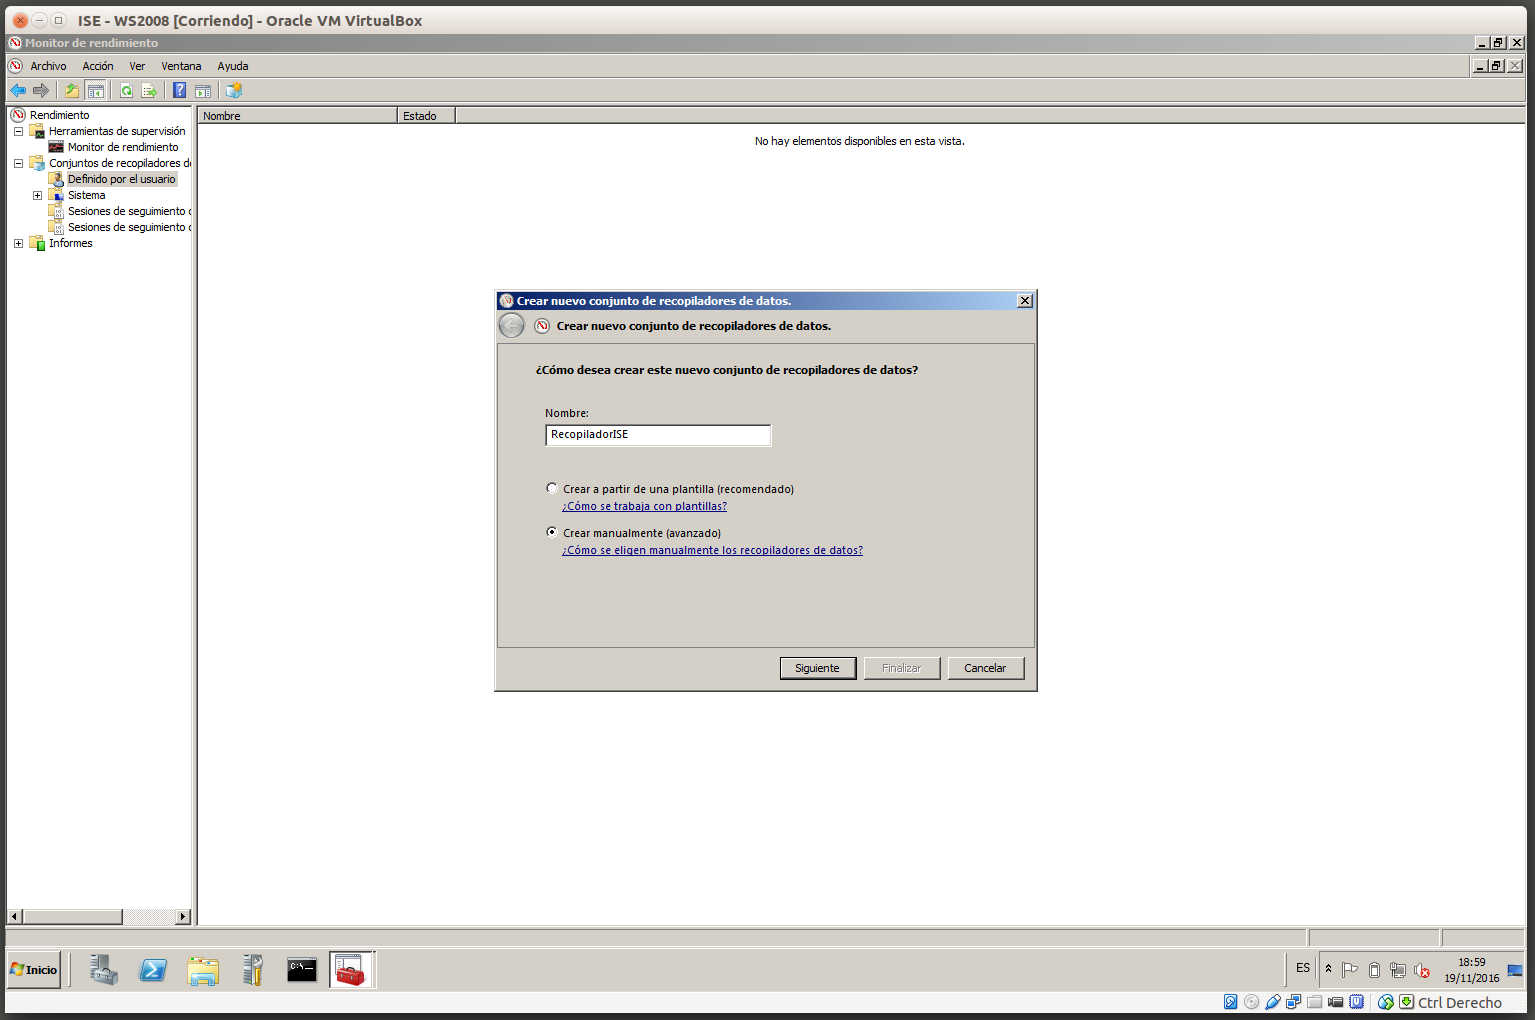
\includegraphics[scale=0.27]{./Imagenes/5-2.png}
		\caption[Elegimos el nombre de nuestro recopilador de datos.]{Elegimos el nombre de nuestro recopilador de datos.}
		\label{5-2}
	\end{figure}
	
	\begin{figure}[H]
		\centering
		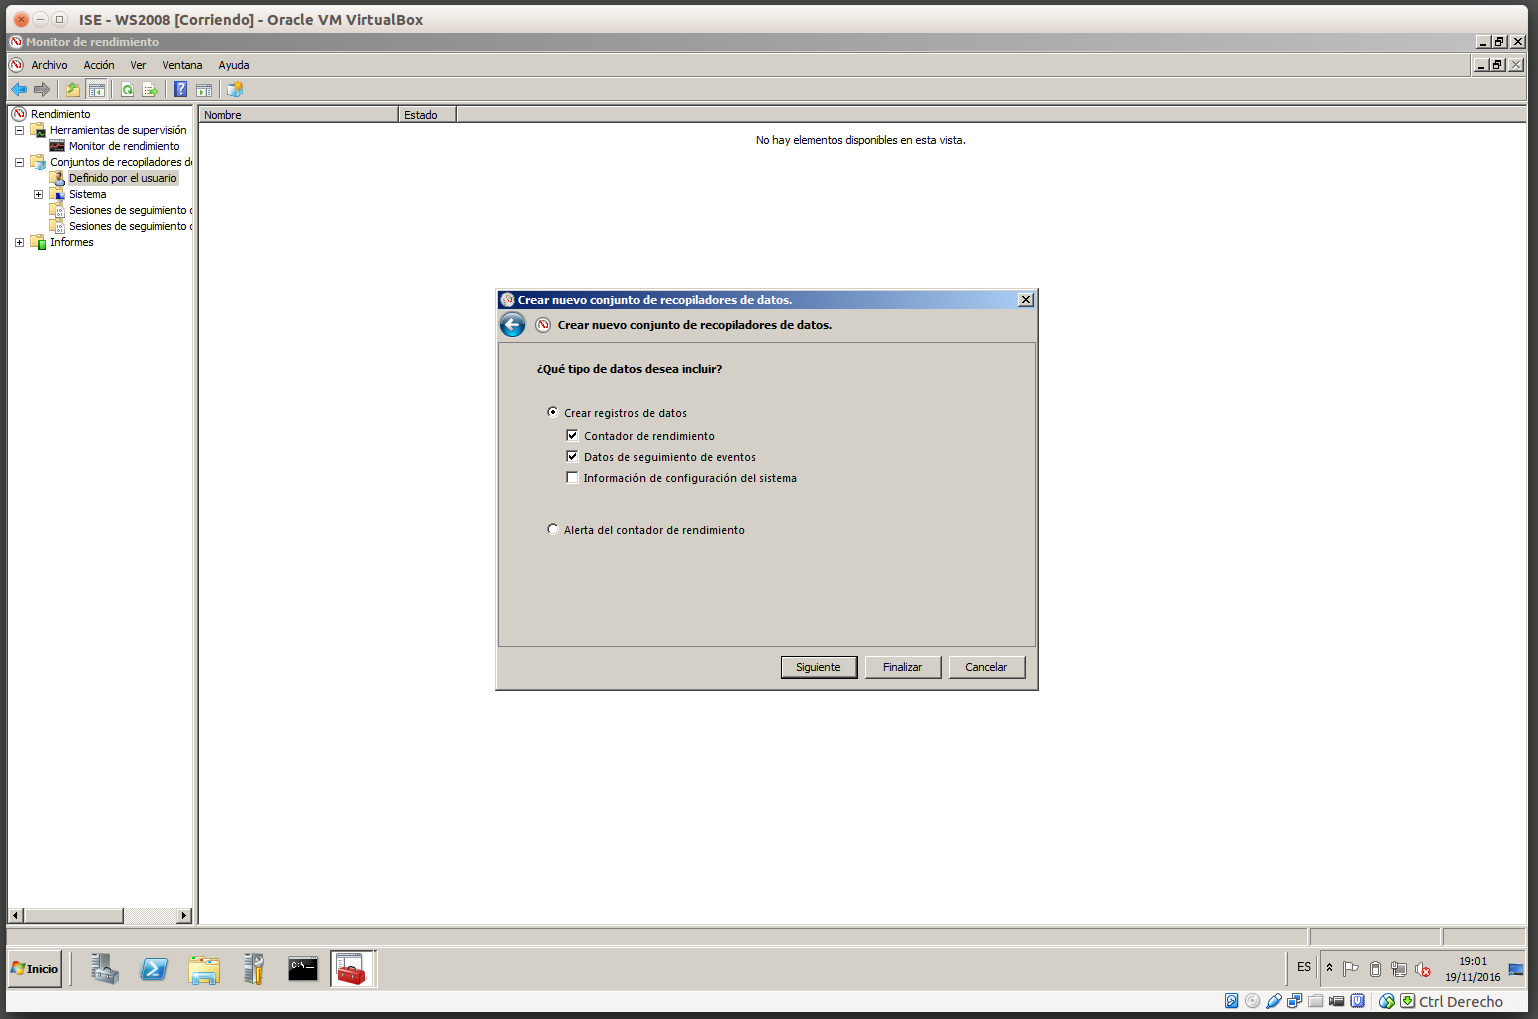
\includegraphics[scale=0.27]{./Imagenes/5-3.png}
		\caption[Elegimos que tipo de datos queremos recopilar.]{Elegimos que tipo de datos queremos recopilar.}
		\label{5-3}
	\end{figure}
	
	\begin{figure}[H]
		\centering
		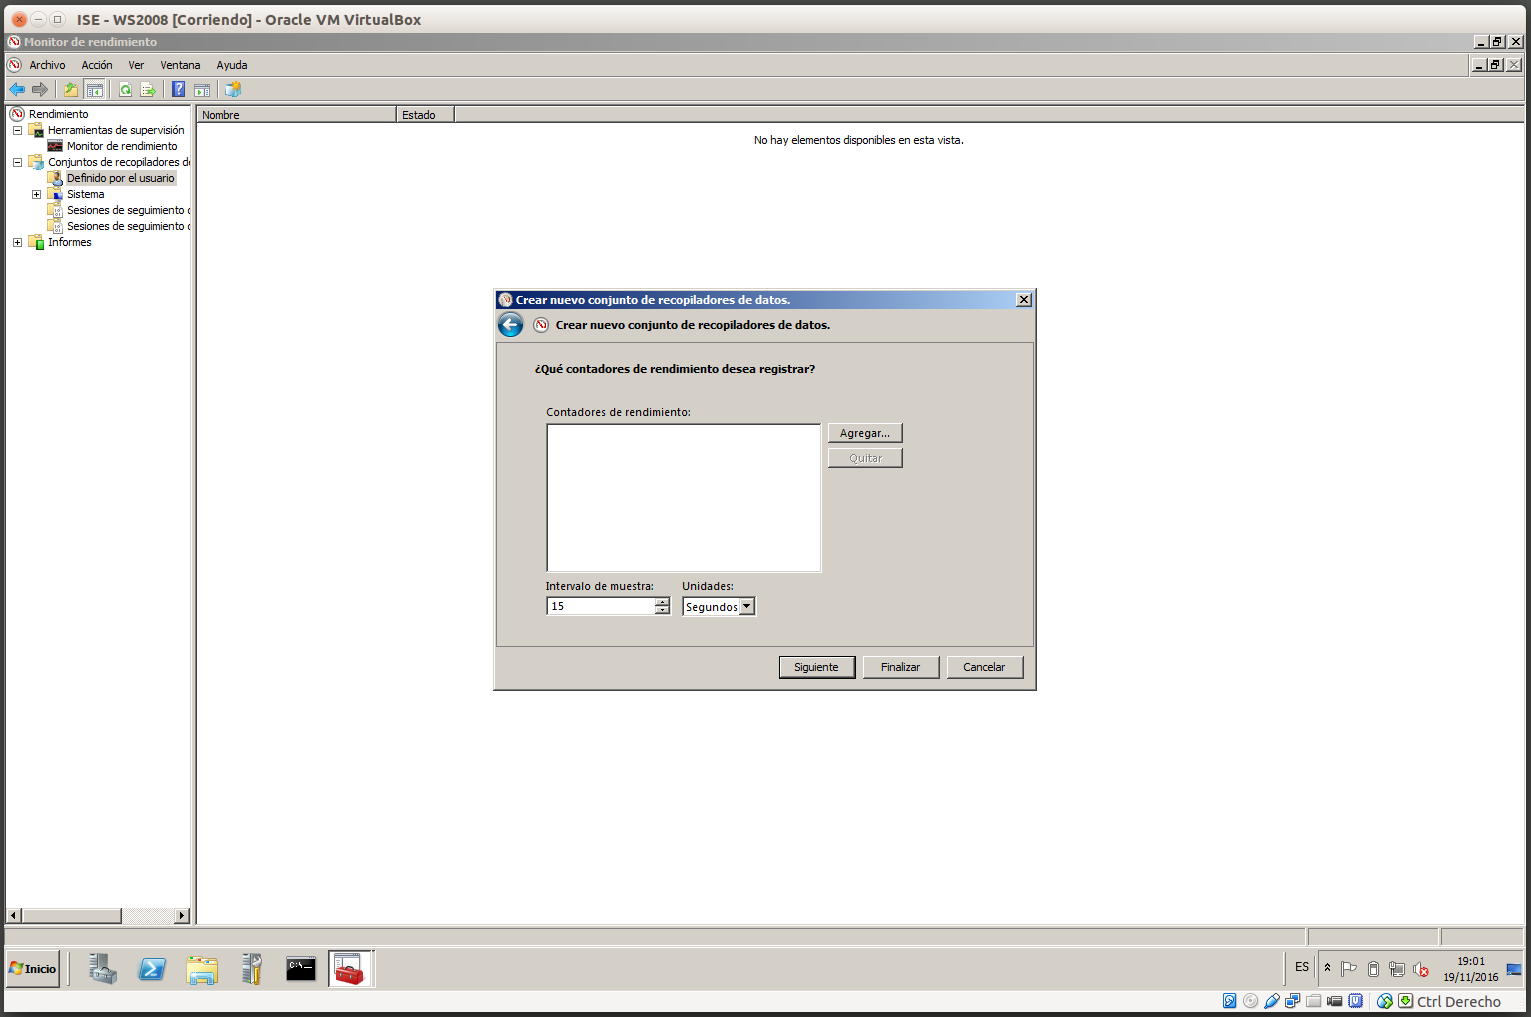
\includegraphics[scale=0.27]{./Imagenes/5-4.png}
		\caption[Elegimos que contadores de rendimiento queremos registrar.]{Elegimos que contadores de rendimiento queremos registrar.}
		\label{5-4}
	\end{figure}
	
	\begin{figure}[H]
		\centering
		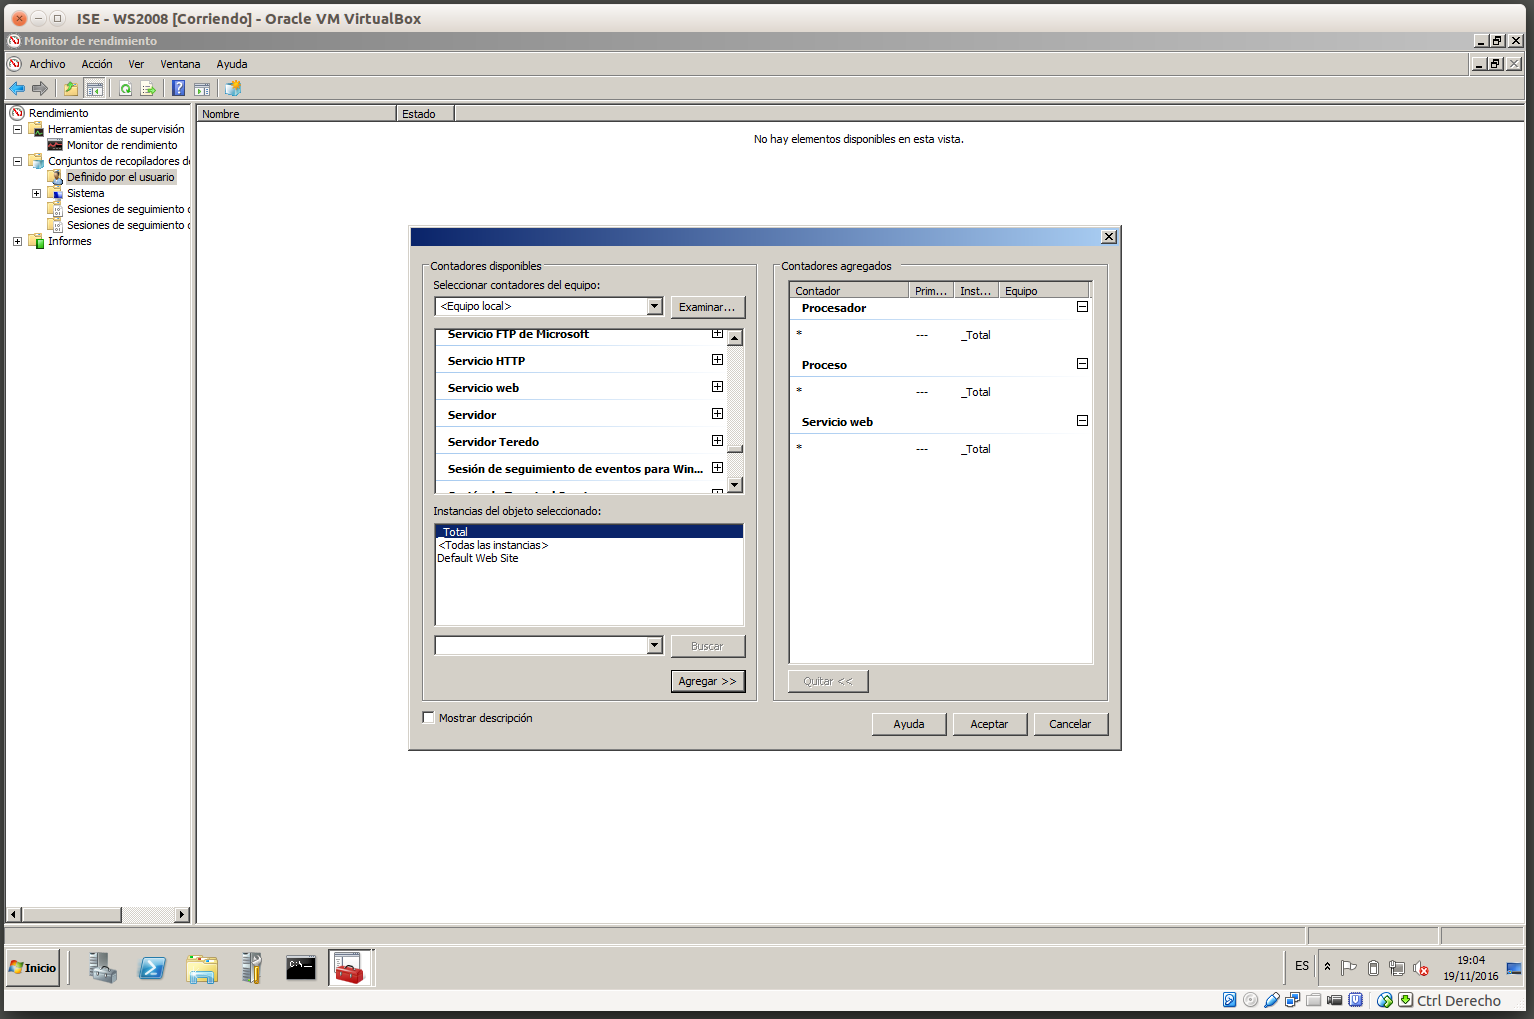
\includegraphics[scale=0.27]{./Imagenes/5-5.png}
		\caption[Datos seleccionados.]{Datos seleccionados.}
		\label{5-5}
	\end{figure}
	
	\begin{figure}[H]
		\centering
		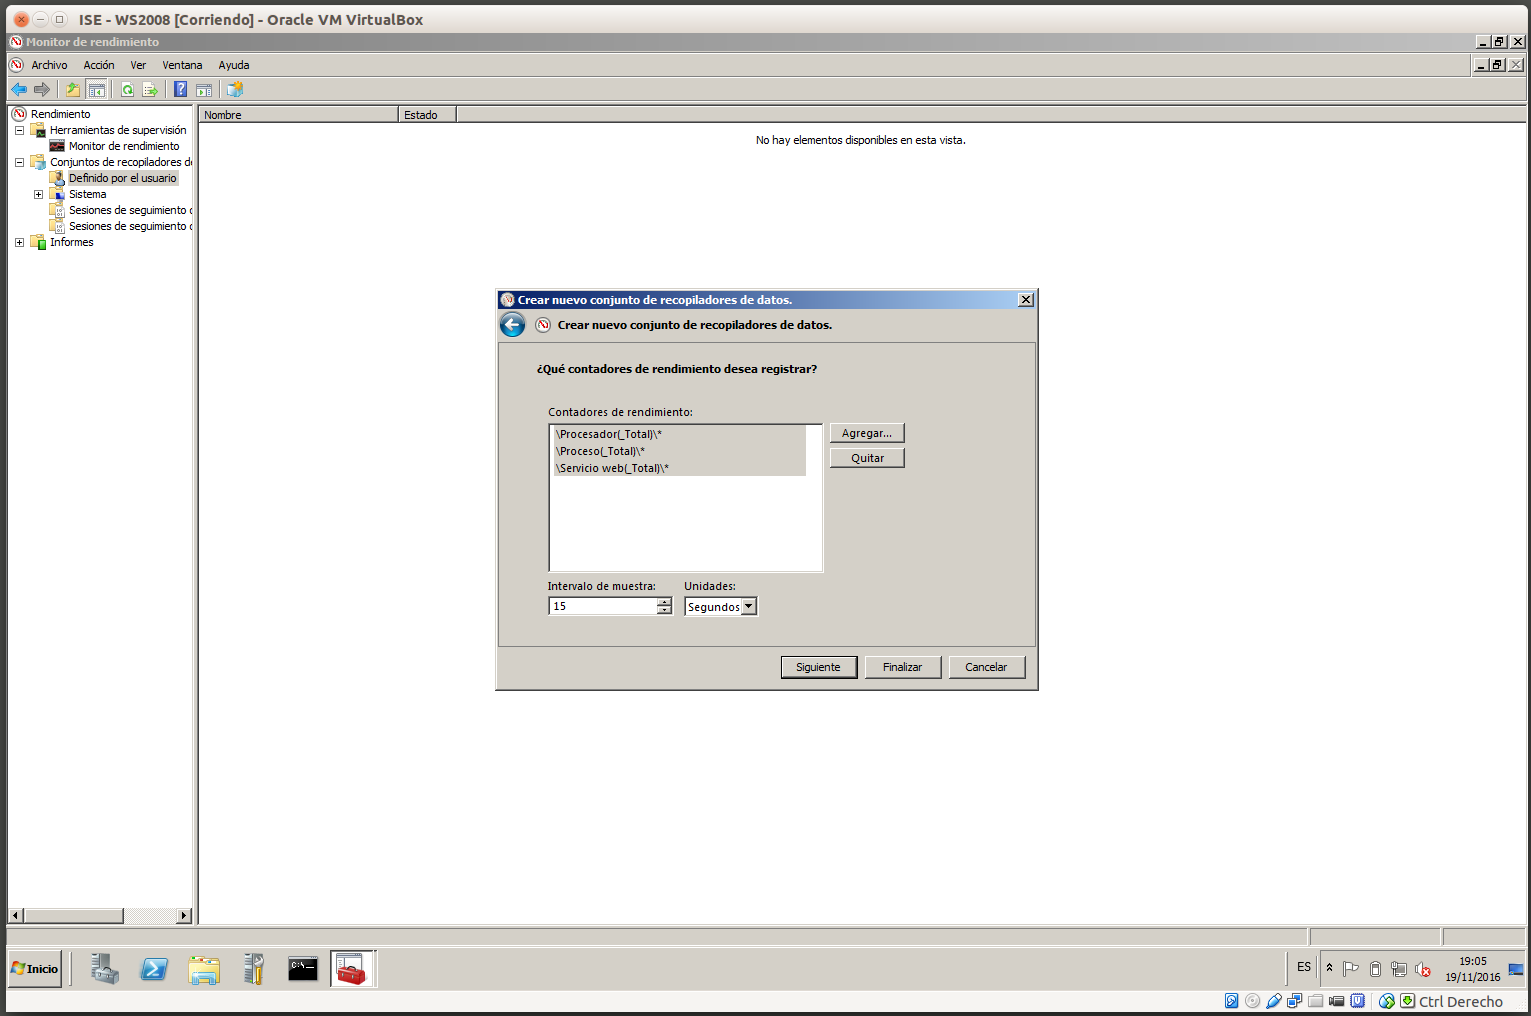
\includegraphics[scale=0.27]{./Imagenes/5-6.png}
		\caption[Elegimos la frecuencia de muestro, 15 segundos en nuestro caso.]{Elegimos la frecuencia de muestro, 15 segundos en nuestro caso.}
		\label{5-6}
	\end{figure}
	
	\begin{figure}[H]
		\centering
		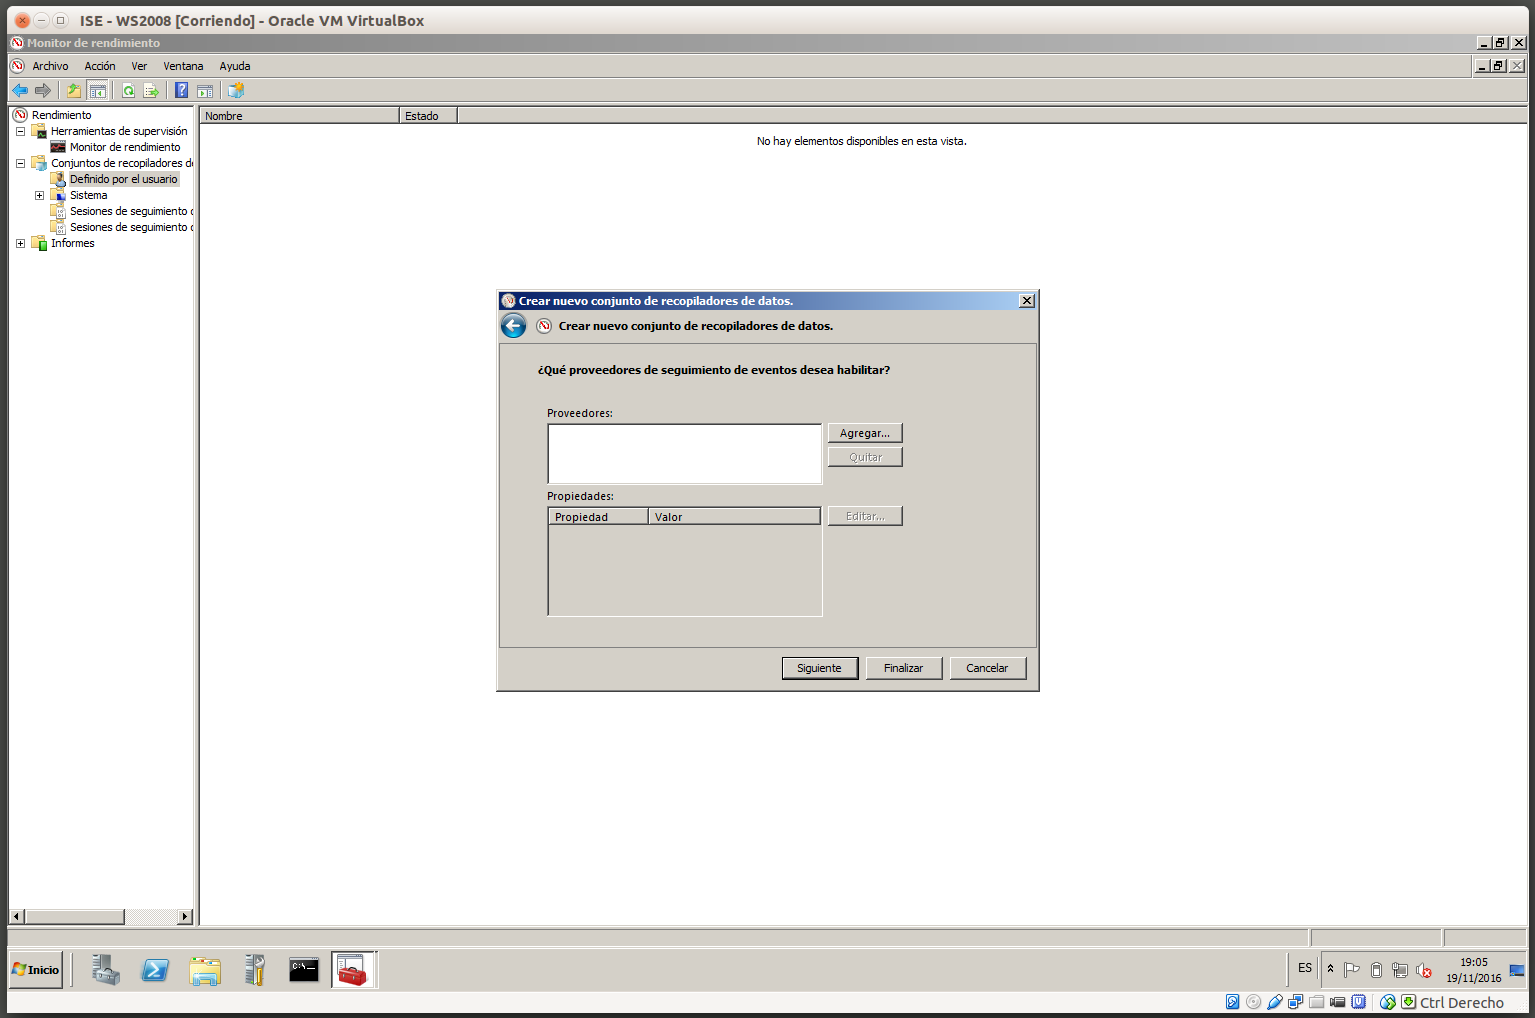
\includegraphics[scale=0.27]{./Imagenes/5-7.png}
		\caption[Dejamos los proveedores de seguimiento de eventos en blanco.]{Dejamos los proveedores de seguimiento de eventos en blanco.}
		\label{5-7}
	\end{figure}
	
	\begin{figure}[H]
		\centering
		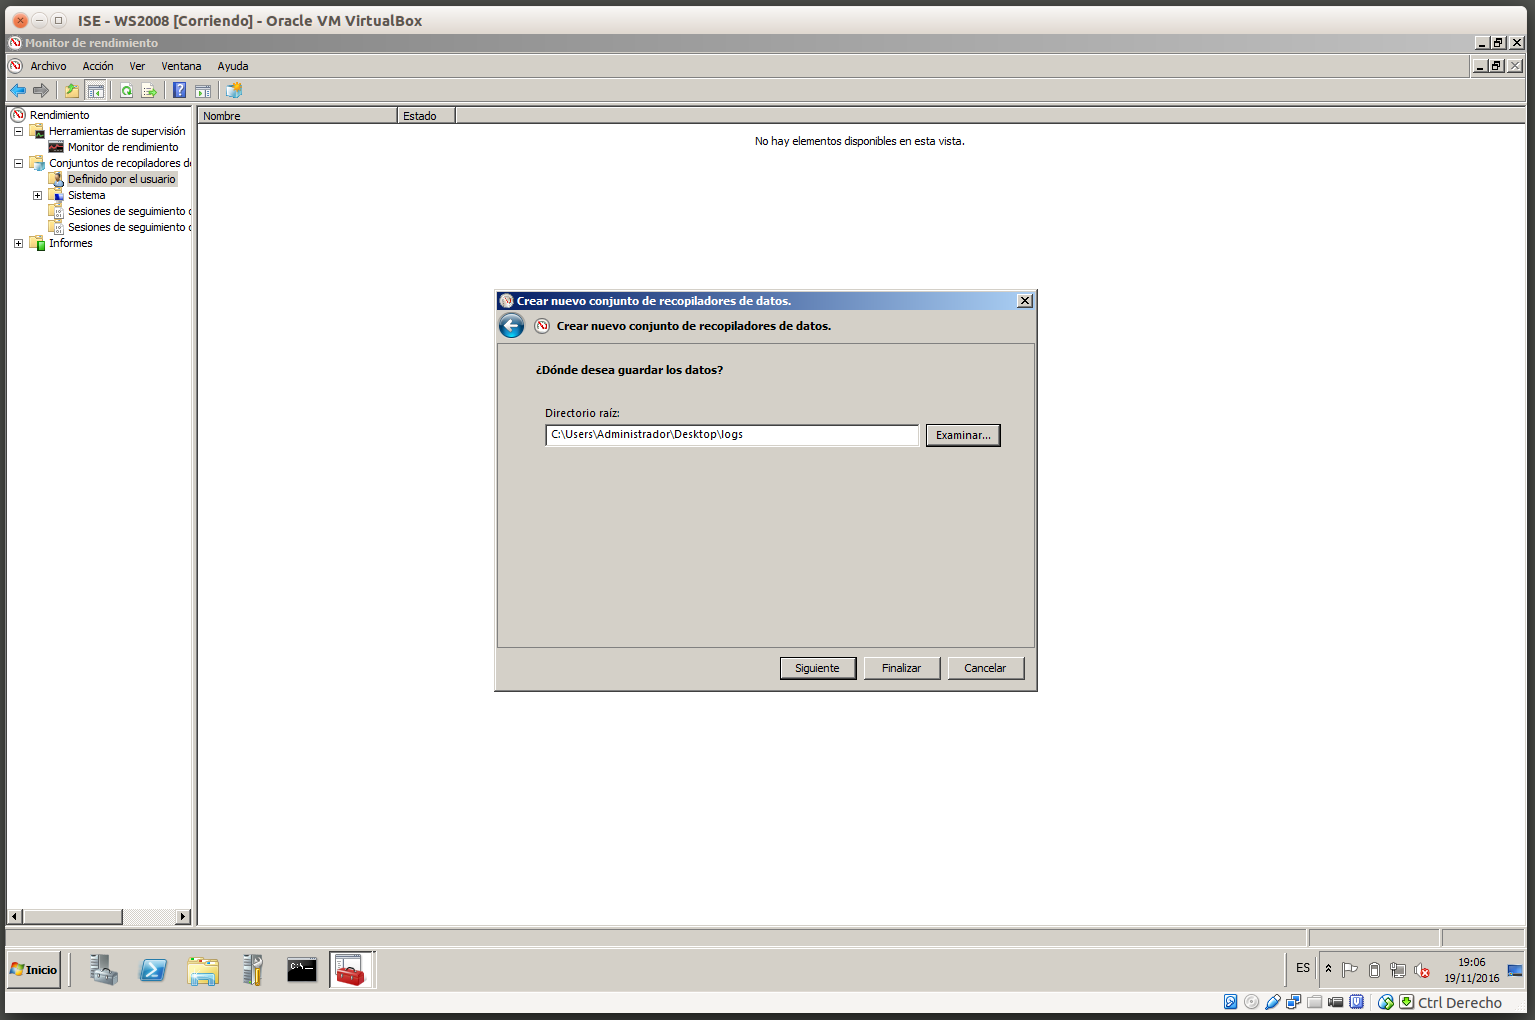
\includegraphics[scale=0.27]{./Imagenes/5-8.png}
		\caption[Guardamos los \textit{logs} en la carpeta \textit{logs} dentro del \textit{Escritorio}.]{Guardamos los \textit{logs} en la carpeta \textit{logs} dentro del \textit{Escritorio}.}
		\label{5-8}
	\end{figure}
	
	\begin{figure}[H]
		\centering
		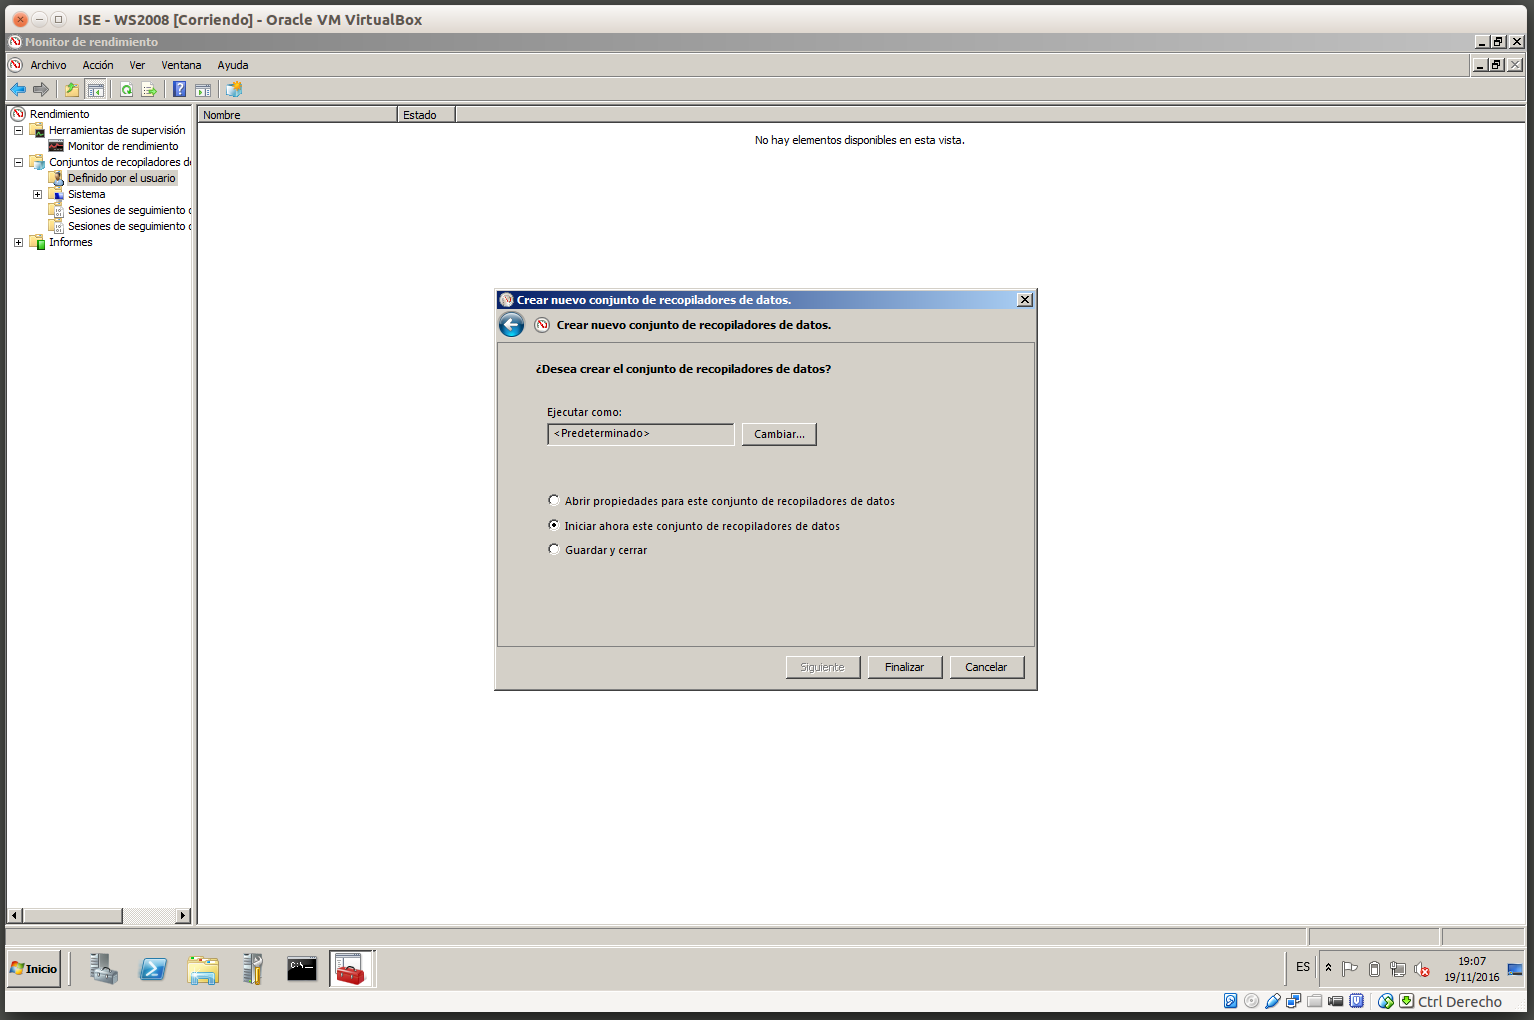
\includegraphics[scale=0.27]{./Imagenes/5-9.png}
		\caption[Elegimos iniciar el recopilador y finalizamos el proceso.]{Elegimos iniciar el recopilador y finalizamos el proceso.}
		\label{5-9}
	\end{figure}

	Una vez hemos creado el recopilador de datos, he generado un análisis para ver que todo funciona correctamente. Para ello he parado el recopilador y lo he puesto de nuevo en funcionamiento. Tras un minuto de análisis, el resultado obtenido lo podemos ver en la figura \ref{5-analisis}. Los primeros 5 segundos de análisis no he hecho nada, por eso no podemos ver nada destacable en la gráfica. Tras esto cinco segundos, he creado abierto un archivo de texto, lo he modificado y lo he guardado. Por eso podemos ver que en el instante de tiempo \textit{20:18:46} empieza a haber datos sobre el número de bytes de lectura y escritura, que son las líneas de color rosa y verde fosforito (las dos seleccionadas en la figura \ref{5-analisis}). El resto de he modificado el archivo pero cambiando menos contenido y lo he ido guardando en distintos momentos del análisis, por eso podemos ver que siguen apareciendo datos sobre bytes de escritura y lectura. Finalmente, he cerrado el archivo y lo he abierto de nuevo, por eso comienza de nuevo a subir el número de bytes leídos (línea de color verde fosforito) en el instante de tiempo \textit{20:19:46}.
	
	\begin{figure}[H]
		\centering
		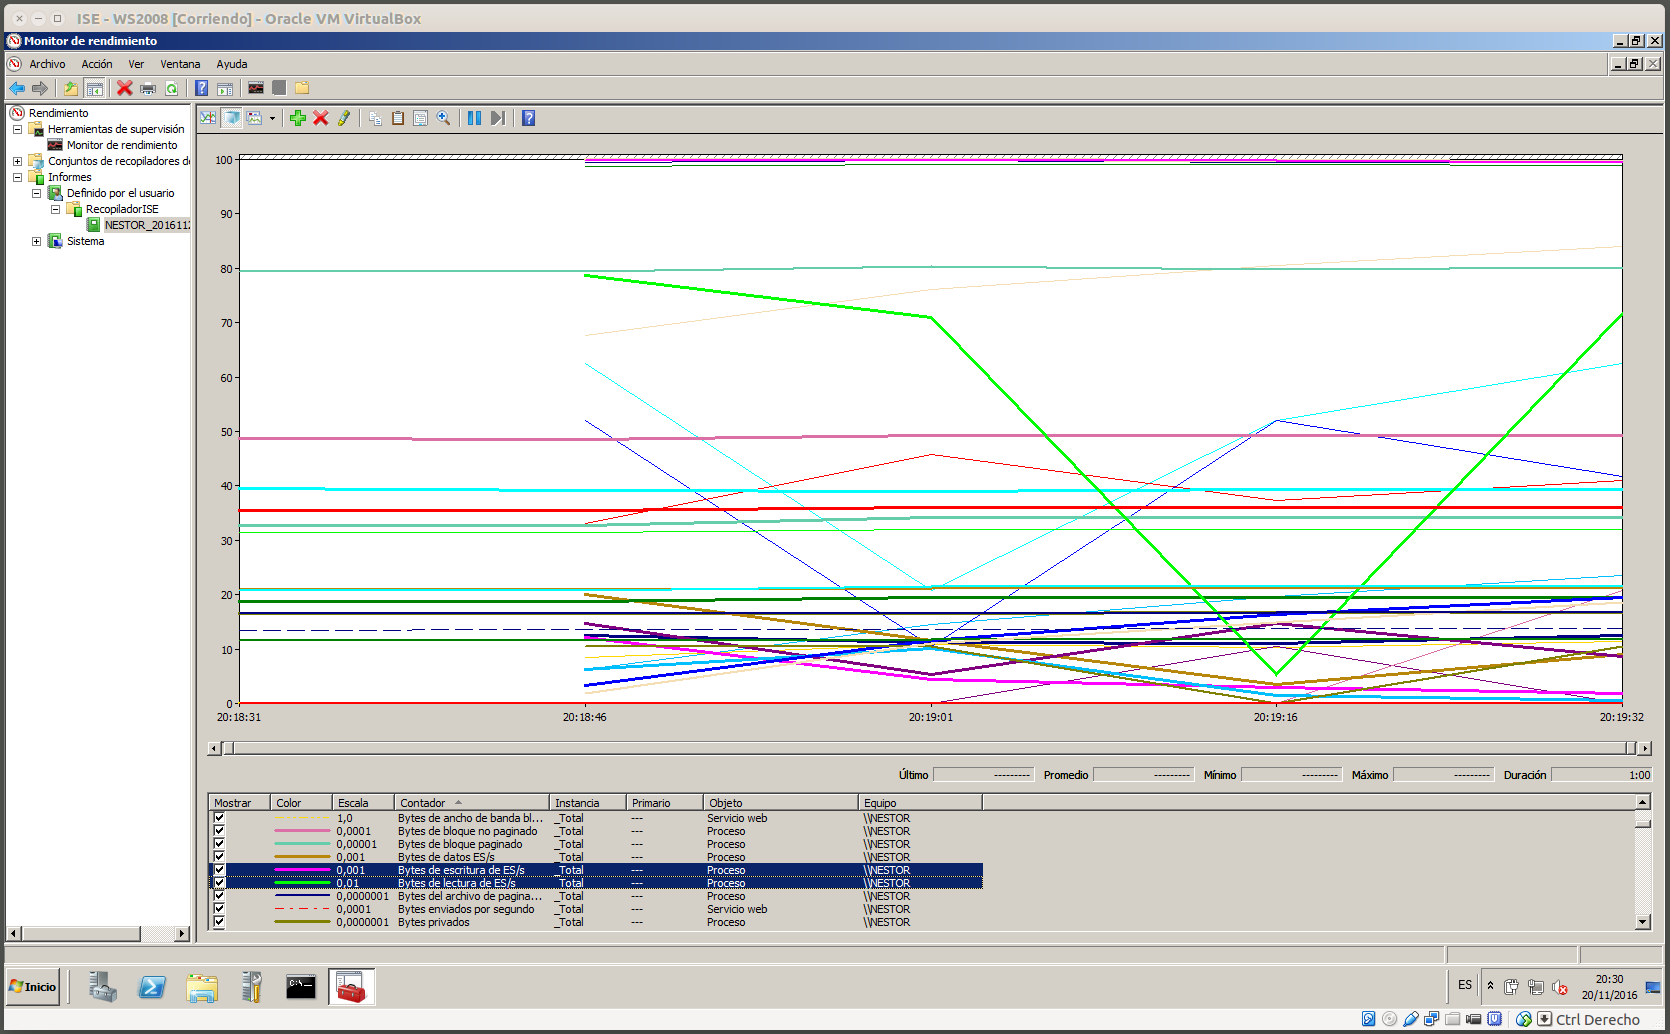
\includegraphics[width=\linewidth]{./Imagenes/5-analisis.png}
		\caption[Resultado obtenido del análisis.]{Resultado obtenido del análisis.}
		\label{5-analisis}
	\end{figure}
	
	%%%%%%%%%%%%%%%%%%%%%%%%%%%%%%%%%%%%%%%%%%%%%%%%%%%%
	%%%%%%%%%%%%%%%%%%%% Cuestión 6 %%%%%%%%%%%%%%%%%%%%
	%%%%%%%%%%%%%%%%%%%%%%%%%%%%%%%%%%%%%%%%%%%%%%%%%%%%
	\section[Cuestión 6: Visite la web del proyecto y acceda a la demo que proporcionan (http://demo.munin-monitoring.org/) donde se muestra cómo monitorizan un servidor. Monitorice varios parámetros y haga capturas de pantalla de lo que está mostrando comentando qué observa.]{Cuestión 6: Visite la web del proyecto y acceda a la demo que proporcionan (http://demo.munin-monitoring.org/) donde se muestra cómo monitorizan un servidor. Monitorice varios parámetros y haga capturas de pantalla de lo que está mostrando comentando qué observa.}
	
	Lo primero que vemos al acceder a la página de la demo de Munin \cite{munin} es que podemos monitorizar muchísimos parámetros distintos, como podemos ver en la figura \ref{6-1}. \\
	
	Yo me he centrado en cuatro parámetros distintos: \textit{entradas y salidas de disco}, \textit{número de hilos}, \textit{interrupciones y cambios de contexto} y \textit{uso de la memoria}. En los datos sobre \textit{entradas y salidas de disco} podemos ver la información recopilada en dos gráficas; en la primera de ellas se recoge los datos del parámetro monitorizado en el día actual y en la segunda los datos de la semana actual. En los tres parámetros restantes podemos ver la información recopilada en cuatro gráficas; en la primera de ellas se recoge los datos del parámetro monitorizado en el día actual, en la segunda los datos de la semana actual, en la tercera los datos del mes actual y en la cuarta los datos del año actual. Pasemos a comentar cada uno de estos parámetros con mas detenimiento. \\
	
	\begin{itemize}
		\item \textbf{Entradas y salidas de disco:} El eje \textit{X} de la gráfica representa el instante de tiempo en el que se han recogido los datos. El eje \textit{Y} de la gráfica representa el número de lecturas de disco si es un valor negativo y el número de escrituras si es un valor positivo. Viendo la gráfica de la figura \ref{6-2} podemos observar que el número de lecturas es notablemente mayor que el número de escrituras.
		\item \textbf{Número de hilos:} El eje \textit{X} de la gráfica representa el instante de tiempo en el que se han recogido los datos. El eje \textit{Y} de la gráfica representa el número de hilos activos en el servidor. Viendo la gráfica de la figura \ref{6-3} podemos observar que el número de hilos, exceptuando los primero días del año, oscila entre 66 y 74 hilos activos.
		\item \textbf{Interrupciones y cambios de contexto:} El eje \textit{X} de la gráfica representa el instante de tiempo en el que se han recogido los datos. El eje \textit{Y} de la gráfica representa el número de interrupciones y cambios de contexto producidos por segundo. En color verde están representados los cambios de contexto y en azul las interrupciones. Viendo la gráfica de la figura \ref{6-4} podemos observar que el número de eventos en este mes se mantiene en el mismo intervalo, entre 100 y 160 eventos por segundo. Pero si observamos la gráfica que nos aporta los datos recopilados en el año actual podemos observar que el número de eventos es de orden creciente, ya que en Enero los mínimos eran de 80 interrupciones, en Febrero el número mínimo de cambios de contexto es de 100 y en Noviembre ambos han crecido hasta 120 y 140 respectivamente.
		\item \textbf{Uso de la memoria:} El eje \textit{X} de la gráfica representa el instante de tiempo en el que se han recogido los datos. El eje \textit{Y} de la gráfica representa el número1 de bytes usados en las operaciones referentes a memoria. Como podemos ver en la figura \ref{6-5} se ha representado con un color cada operación, para poder diferenciarlas visualmente con facilidad. También podemos observar que la mayoría del uso de la memoria se debe a la \textit{memoria virtual comprometida} (119.22M en el momento actual). Lo que menos repercute en el uso de la memoria es la cantidad total de memoria virtual usada, \textit{vmalloc\_used} (508K en el momento actual).
	\end{itemize}
	
	\begin{figure}[H]
		\centering
		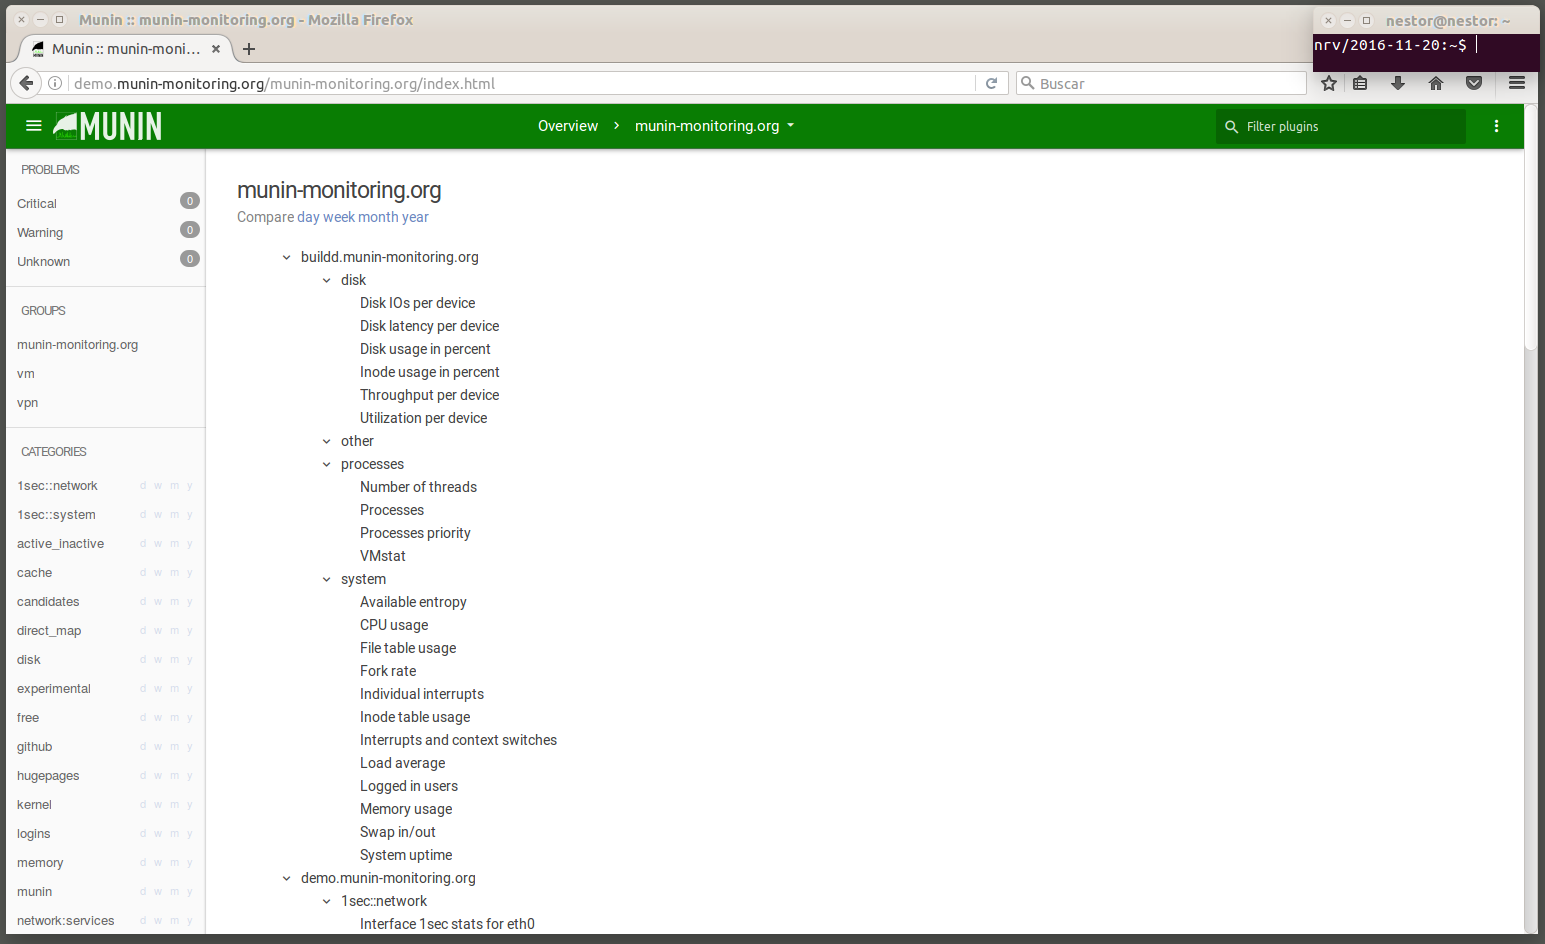
\includegraphics[scale=0.28]{./Imagenes/6-1.png}
		\caption[Parte de los parámetros disponibles para monitorizar.]{Parte de los parámetros disponibles para monitorizar.}
		\label{6-1}
	\end{figure}
	
	\begin{figure}[H]
		\centering
		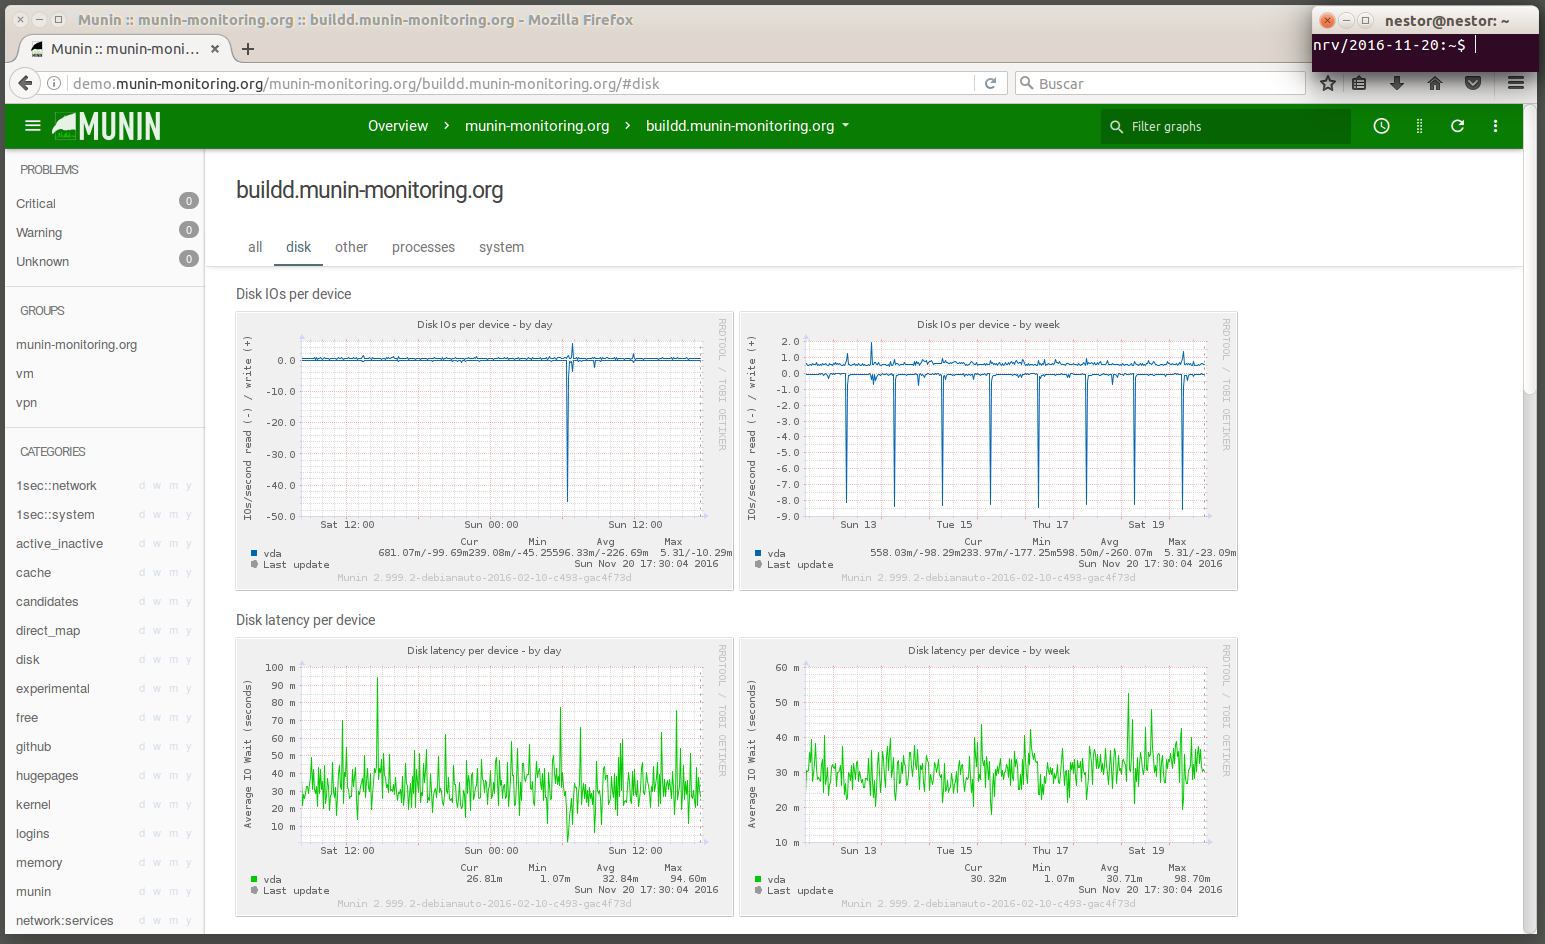
\includegraphics[scale=0.28]{./Imagenes/6-2.png}
		\caption[Entradas y salidas de disco.]{Entradas y salidas de disco.}
		\label{6-2}
	\end{figure}
	
	\begin{figure}[H]
		\centering
		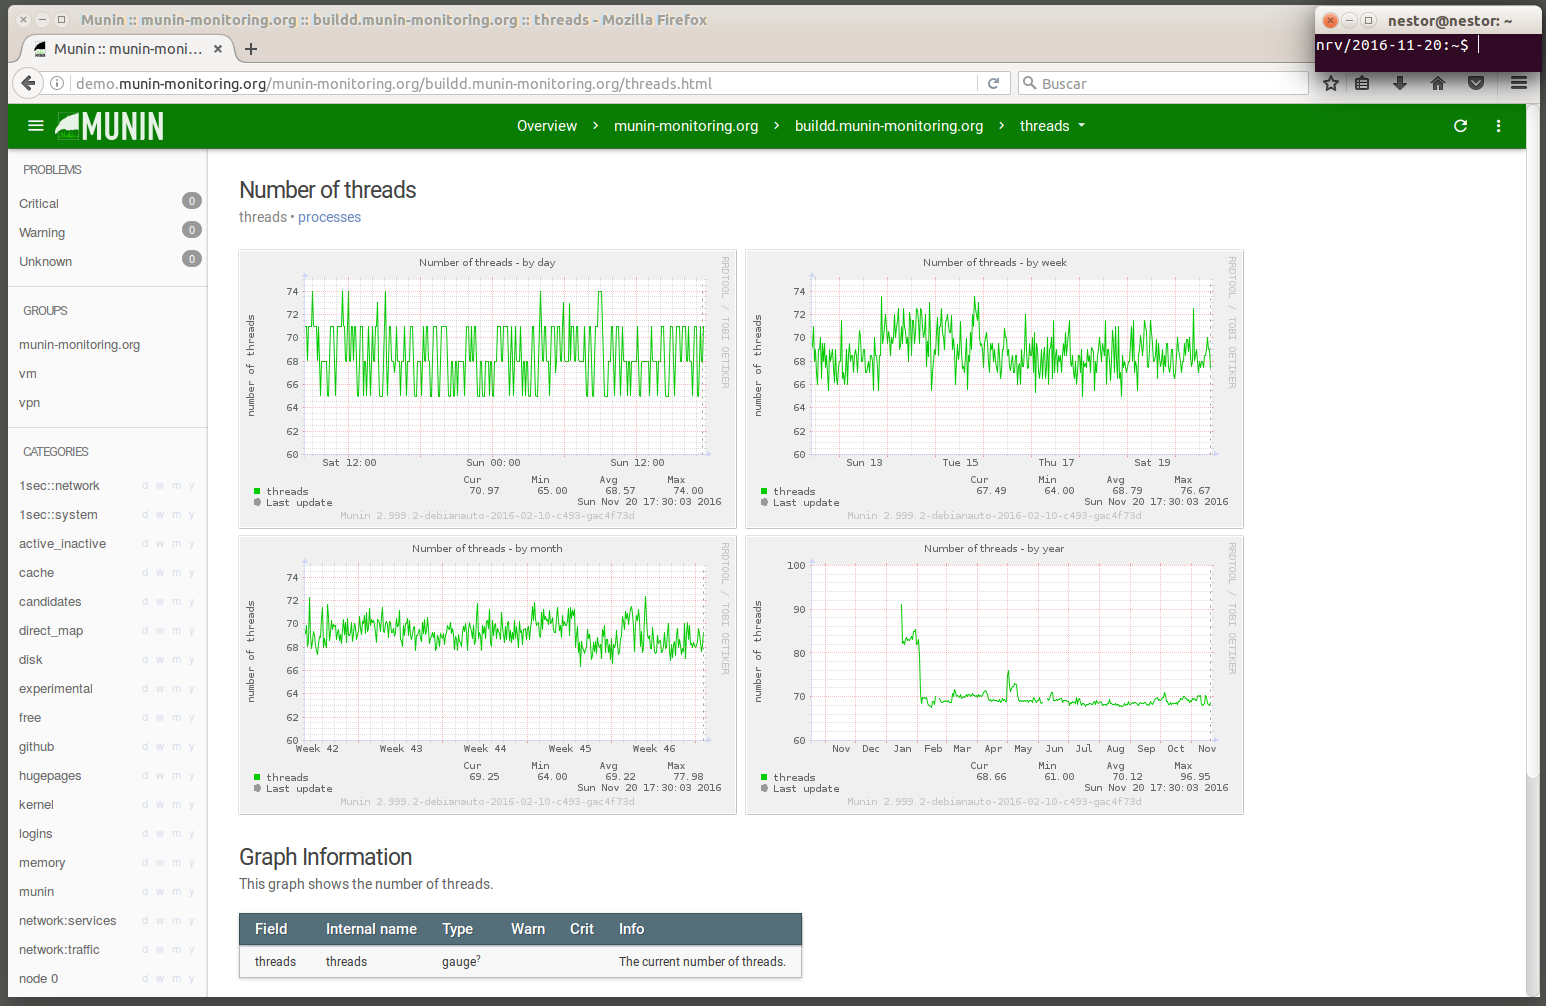
\includegraphics[scale=0.27]{./Imagenes/6-3.png}
		\caption[Número de hilos.]{Número de hilos.}
		\label{6-3}
	\end{figure}
	
	\begin{figure}[H]
		\centering
		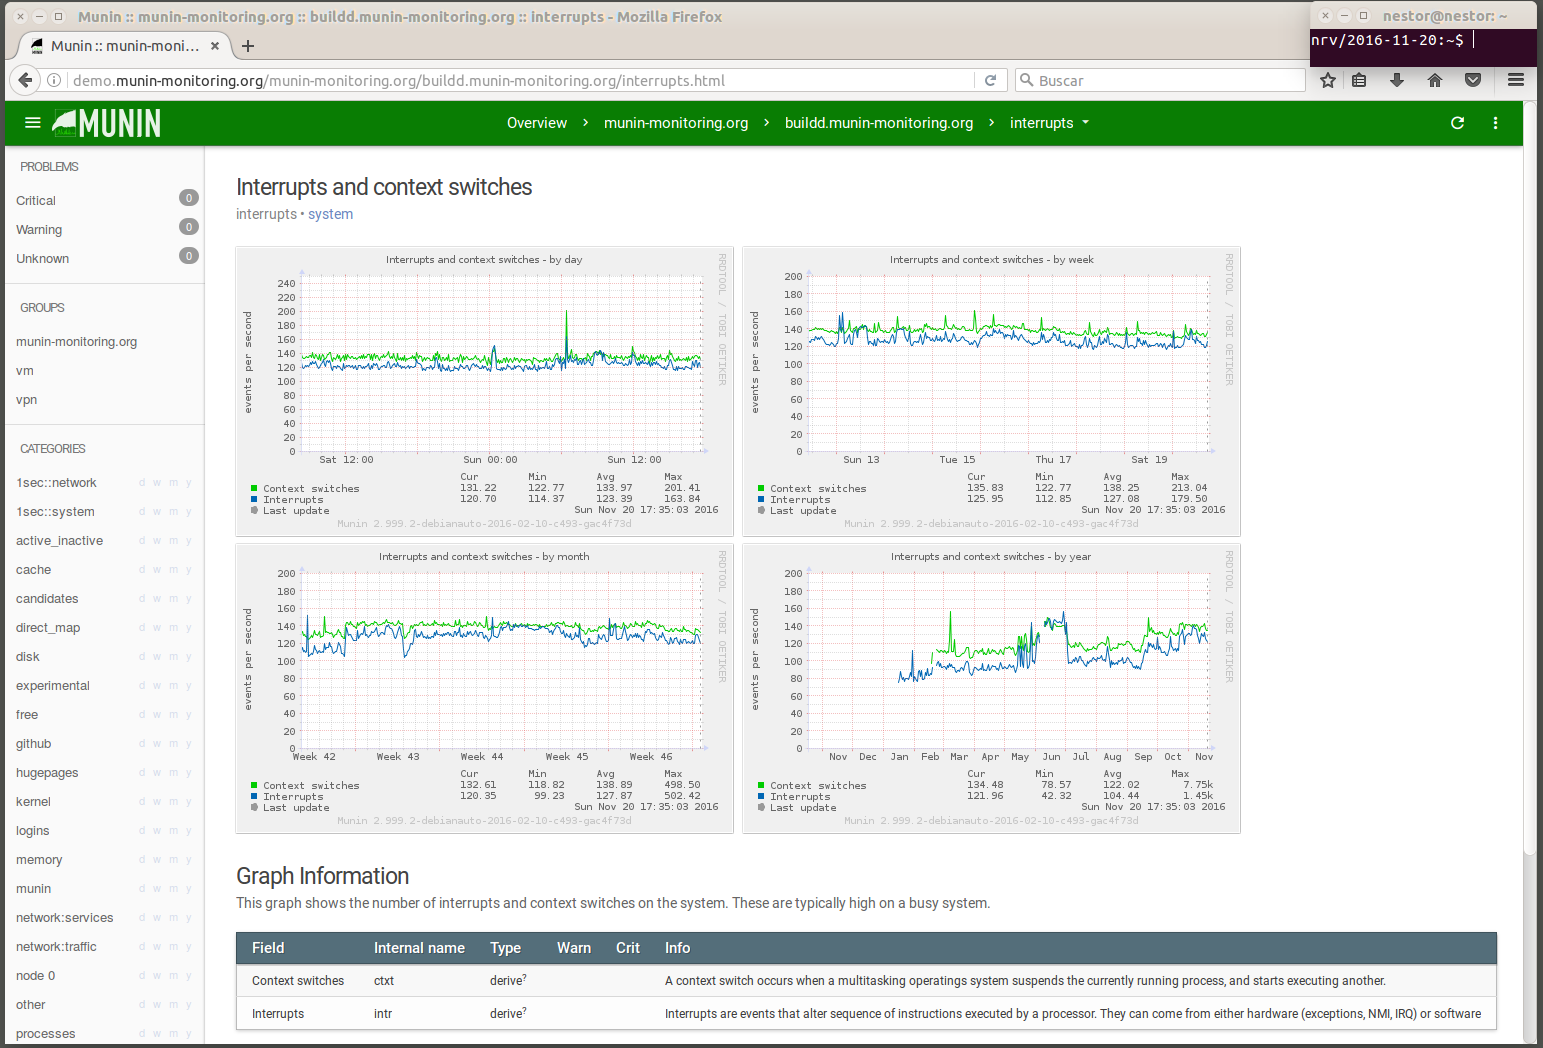
\includegraphics[scale=0.27]{./Imagenes/6-4.png}
		\caption[Interrupciones y cambios de contexto.]{Interrupciones y cambios de contexto.}
		\label{6-4}
	\end{figure}
	
	\begin{figure}[H]
		\centering
		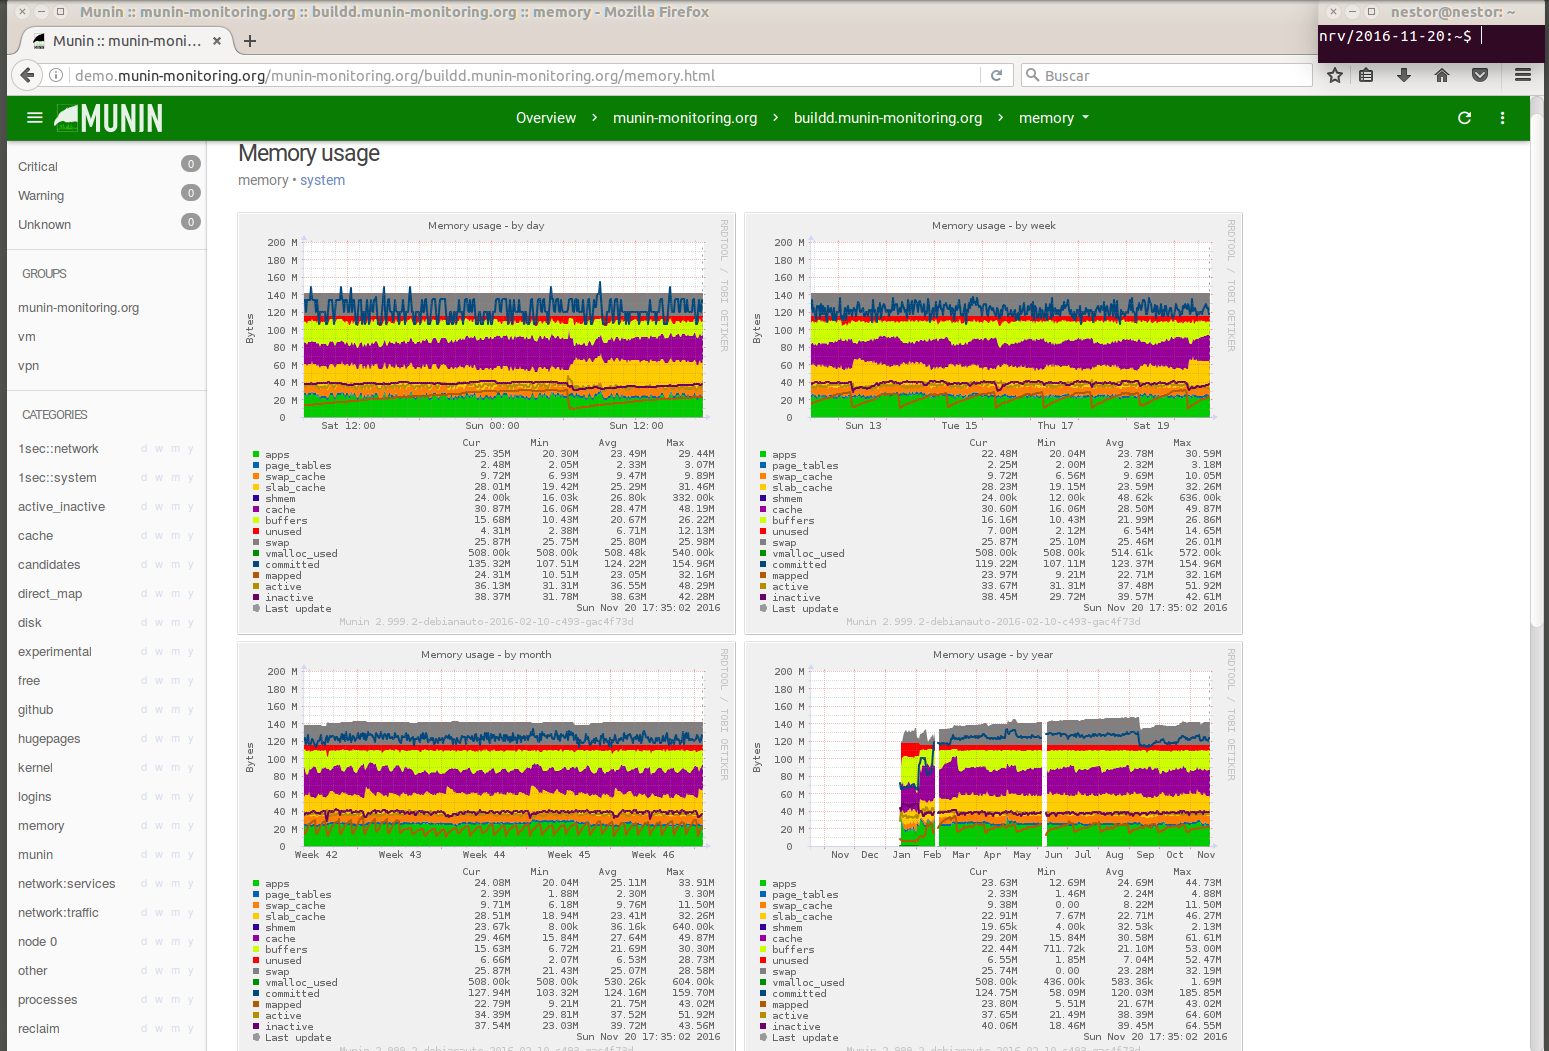
\includegraphics[scale=0.27]{./Imagenes/6-5.png}
		\caption[Uso de la memoria.]{Uso de la memoria.}
		\label{6-5}
	\end{figure}
	
	%%%%%%%%%%%%%%%%%%%%%%%%%%%%%%%%%%%%%%%%%%%%%%%%%%%%
	%%%%%%%%%%%%%%%%%%%% Cuestión 7 %%%%%%%%%%%%%%%%%%%%
	%%%%%%%%%%%%%%%%%%%%%%%%%%%%%%%%%%%%%%%%%%%%%%%%%%%%
	\section[Cuestión 7: Escriba un breve resumen sobre alguno de los artículos donde se muestra el uso de strace o busque otro y coméntelo.]{Cuestión 7: Escriba un breve resumen sobre alguno de los artículos donde se muestra el uso de strace o busque otro y coméntelo.}
	
	El artículo que voy a comentar es uno de los dos que se nos ha dado en el guió de prácticas. El que he elegido es el del blog \textit{Softlayer} \cite{strace}. \\
	
	Lo primero a tratar es que es \textit{strace}, como bien aclara el artículo, no es un depurador, es una herramienta para programadores. Se usa para monitorizar las llamadas del sistema y las señales producidas en la ejecución de un programa. El uso de \textit{strace} es bastante sencillo, lo único que hay que hacer es ``adjuntar'' \textit{strace} a la ejecución de nuestro programa. Por ejemplo, si queremos ver que ocurre cuando se ejecuta \textit{ls} sobre el directorio \textit{/home} sólo debemos ejecutar \textit{strace ls /home}. Esto nos mostrará por pantalla todo lo sucedido internamente. Esta aplicación de \textit{strace} puede ser un poco básica, aunque bien sirve como ejemplo didáctico. Lee, escritor del artículo de \textit{Softlayer} \cite{strace} nos comenta algunos ejemplos que podría tener \textit{strace} en la vida real. De los dos ejemplos que explica, el que más me ha gustado ha sido el segundo, así que voy a comentarlo con más detenimiento. \\
	
	\textit{strace} puede ser usado para encontrar errores. Cuando una llamada a una función falla, \textit{strace} devuelve una línea con `` = -1'' en la salida. Por ejemplo, intentamos iniciar \textit{Apache} pero este no se inicia y no sabemos porque. Para encontrar el problema, podemos usar \textit{strace} de la siguiente manera;: \textit{strace -Ff -o output.txt -e open /etc/init.d/httpd start} \footnote{El argumento \textit{-Ff} es para seguir todos los subprocesos hijo. El argumento \textit{-o} es para redirigir la salida a un fichero. EL argumento \textit{-e} es para mostrar sólo las llamadas a funciones que se indica tras el argumento, \textit{open} en este caso.}. \textit{Apache} intentara iniciarse y \textit{strace} hará su trabajo. Una vez acabado el intento de inicio, sólo debemos aplicar \textit{grep '= -1'} sobre el fichero al que hemos redirigido la salida de \textit{strace} y ver que ha sucedido. En el blog \textit{Softlayer} tenemos el contenido de dicho fichero. Si nos fijamos en la última línea de ese fragmento, podemos ver lo siguiente: \textit{[pid 13748] open(``/etc/httpd/logs/error\_log'', O\_WRONLY$\mid$O\_CREAT$\mid$O\_APPEND$\mid$O\_LARGEFILE, 0666) = -1 EACCES (Permission denied)}, es decir, no se tiene permiso para abrir el archivo \textit{/etc/httpd/logs/error\_log}. Si ahora inspeccionamos los permisos de dicho fichero, podemos ver que tiene el atributo de inmutable, y eso es lo que causa el error. \\
	
	Como dice Lee, gracias a \textit{strace} podemos encontrar errores que de otro modo no encontraríamos o tardaríamos mucho tiempo en darnos cuenta de a que se debe el error.
	
	%%%%%%%%%%%%%%%%%%%%%%%%%%%%%%%%%%%%%%%%%%%%%%%%%%%%
	%%%%%%%%%%%%%%%%%%%% Cuestión 8 %%%%%%%%%%%%%%%%%%%%
	%%%%%%%%%%%%%%%%%%%%%%%%%%%%%%%%%%%%%%%%%%%%%%%%%%%%
	\section[Cuestión 8: Escriba un script en Python o PHP y analice su comportamiento usando el profiler presentado.]{Cuestión 8: Escriba un script en Python o PHP y analice su comportamiento usando el profiler presentado.}
	
	El script que voy a usar es el script \footnote{El script \textit{``8-profiler.py''} se encuentra dentro de la carpeta \textit{Archivos auxiliares}.} \ref{8-script_python}.
		
	%Pongo que el lenguaje es bash y no pyhton porque con python no me gusta como queda estéticamente.
	\begin{lstlisting}[language=bash, label={8-script_python}]
#!/usr/bin/python

suma = 0

for i in range(100):
if i%2 != 0:
print i,
suma += i
print `La suma es: % i' % suma
	\end{lstlisting}
		
	La prueba la voy a hacer en Ubuntu Server. El script lo he ubicado en \textit{/home/nestor}, como se puede ver en la figura \ref{8-script}.
	\begin{figure}[H]
		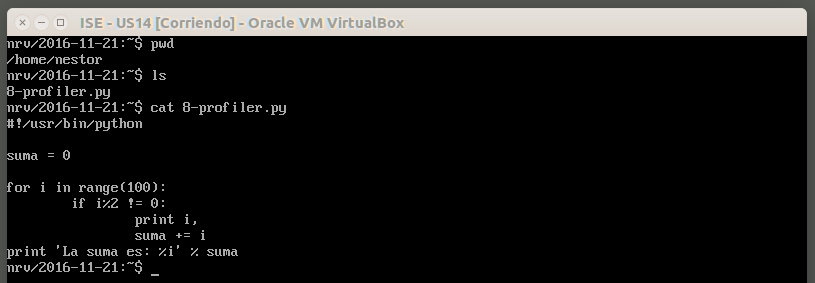
\includegraphics[width=\linewidth]{./Imagenes/8-script.png}
		\vspace{-0.5cm}
		\caption[Script que imprime los números impares entre 0 y 100 y los suma.]{Script que imprime los números impares entre 0 y 100 y los suma.}
		\label{8-script}
	\end{figure}
		
	Como bien nos recomienda el ejercicio, el profiler que voy a usar es \textit{CProfile} \cite{cprofile}. Para ejecutar el programa usando el profiler, debemos ejecutar \textit{python -m cProfile 8-profiler.py}. El resultado lo podemos ver en la figura \ref{8-profiler}.
	
	\begin{figure}[H]
		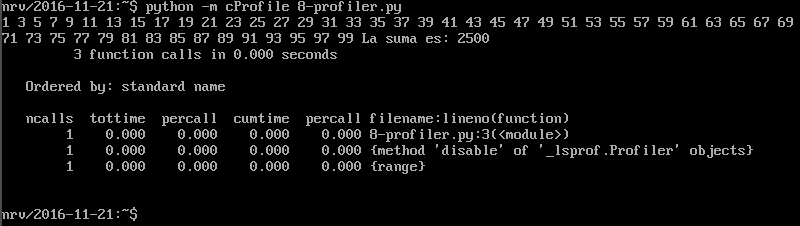
\includegraphics[width=\linewidth]{./Imagenes/8-profiler.png}
		\vspace{-0.5cm}
		\caption[Resultado del profiler.]{Resultado del profiler.}
		\label{8-profiler}
	\end{figure}
	
	La primera información que podemos ver es que se han producido 3 llamadas a funciones y que el programa ha tardado 0.000 segundos. A continuación podemos ver que criterio se ha usado para ordenar las funciones, en este caso se han ordenado por nombre estándar. Finalmente, podemos ver una tabla que tiene 6 columnas y 3 filas (una fila por cada función que ha sido llamada). El significado de las columnas es \cite{cprofile}:
	\begin{itemize}
		\item \textbf{ncalls:} Número de veces que se llama a la función. En mi caso todas las funciones han sido llamadas una única vez. 
		\item \textbf{tottime:} Tiempo total de la función excluyendo llamadas a subfunciones.
		\item \textbf{percall:} Cociente de \textit{tottime} entre \textit{ncalls.}
		\item \textbf{cumtime:} Tiempo acumulado en la función y todas las subfunciones.
		\item \textbf{percall:} Cociente de \textit{cumtime} entre las llamadas primitivas.
		\item \textbf{filename:lineno(function):} Información sobre la función, como el archivo donde se encuentra, la línea donde está y el nombre de la función.
	\end{itemize}
	
	%%%%%%%%%%%%%%%%%%%%%%%%%%%%%%%%%%%%%%%%%%%%%%%%%%%%
	%%%%%%%%%%%%%%%%%%%% Cuestión 9 %%%%%%%%%%%%%%%%%%%%
	%%%%%%%%%%%%%%%%%%%%%%%%%%%%%%%%%%%%%%%%%%%%%%%%%%%%
	\section[Acceda a la consola mysql (o a través de phpMyAdmin) y muestre el resultado de mostrar el ``profile'' de una consulta (la creación de la BD y la consulta la puede hacer libremente).]{Acceda a la consola mysql (o a través de phpMyAdmin) y muestre el resultado de mostrar el ``profile'' de una consulta (la creación de la BD y la consulta la puede hacer libremente).}
	
	Como bien pone en el guión, para aprender a usar el profiler de MySQL me he fijado en las dos secciones que hablan acerca de ello en la página de MySQL \cite{mysql} \cite{mysql2}. Yo lo voy a hacer con phpMyAdmin, así que lo primero que hago es conectarme a mi servidor y entrar a phpMyAdmin. Para ello escribimos en el buscador de mi máquina local la dirección IP de mi servidor seguido de \textit{/phpmyadmin}. En mi caso debemos escribir \textit{192.168.56.103/phpmyadmin}, como podemos ver en la figura \ref{9-1}.

	\begin{figure}[H]
		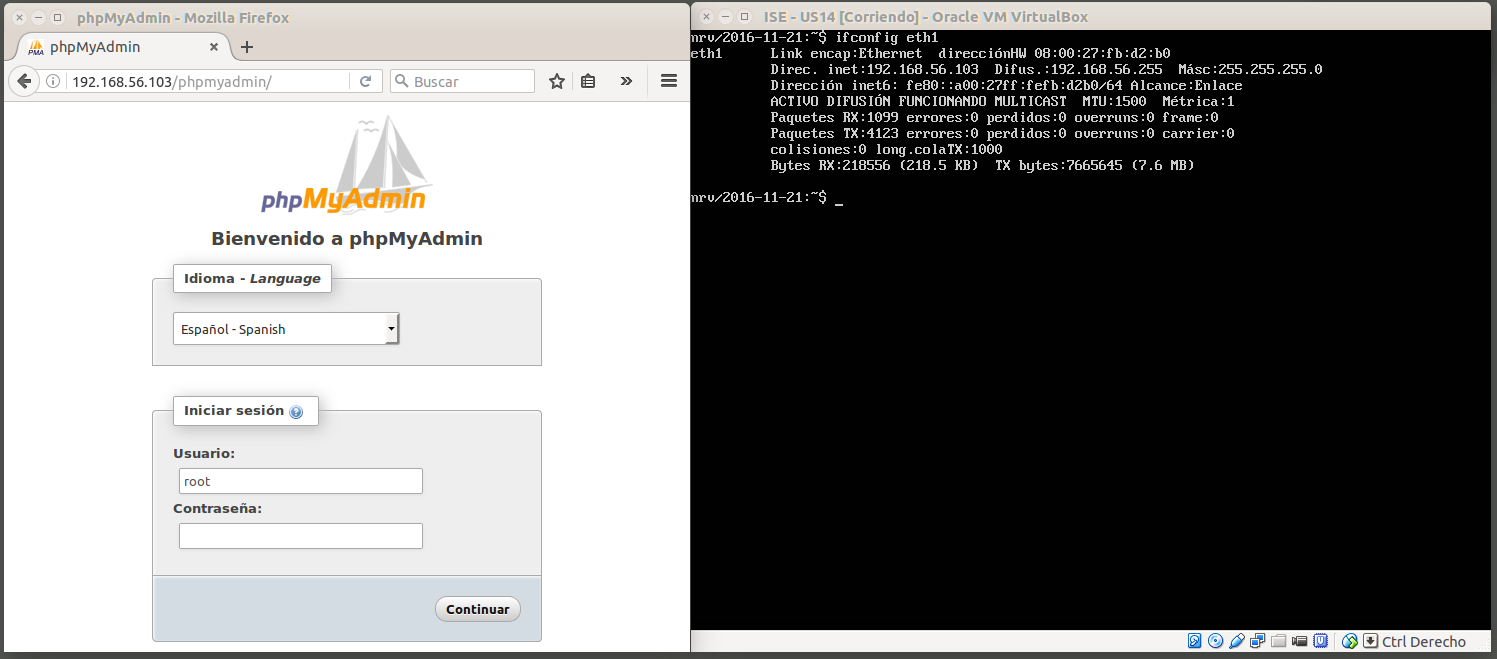
\includegraphics[width=\linewidth]{./Imagenes/9-1.png}
		\vspace{-0.5cm}
		\caption[Conexión con phpMyAdmin (máquinas conectadas en modo \textit{host-only}).]{Conexión con phpMyAdmin (máquinas conectadas en modo \textit{host-only}).}
		\label{9-1}
	\end{figure}
	
	Una vez nos conectamos, abrimo una consola de SQL y ejecutamos las siguientes sentencias, como se puede ver en la figura \ref{9-2}:
	\begin{itemize}
		\item CREATE DATABASE EJ9;
		\item USE EJ9;
		\item CREATE TABLE tabla (dato1 INT, dato2 INT);
		\item SET profiling=1;
	\end{itemize}
	
	\begin{figure}[H]
		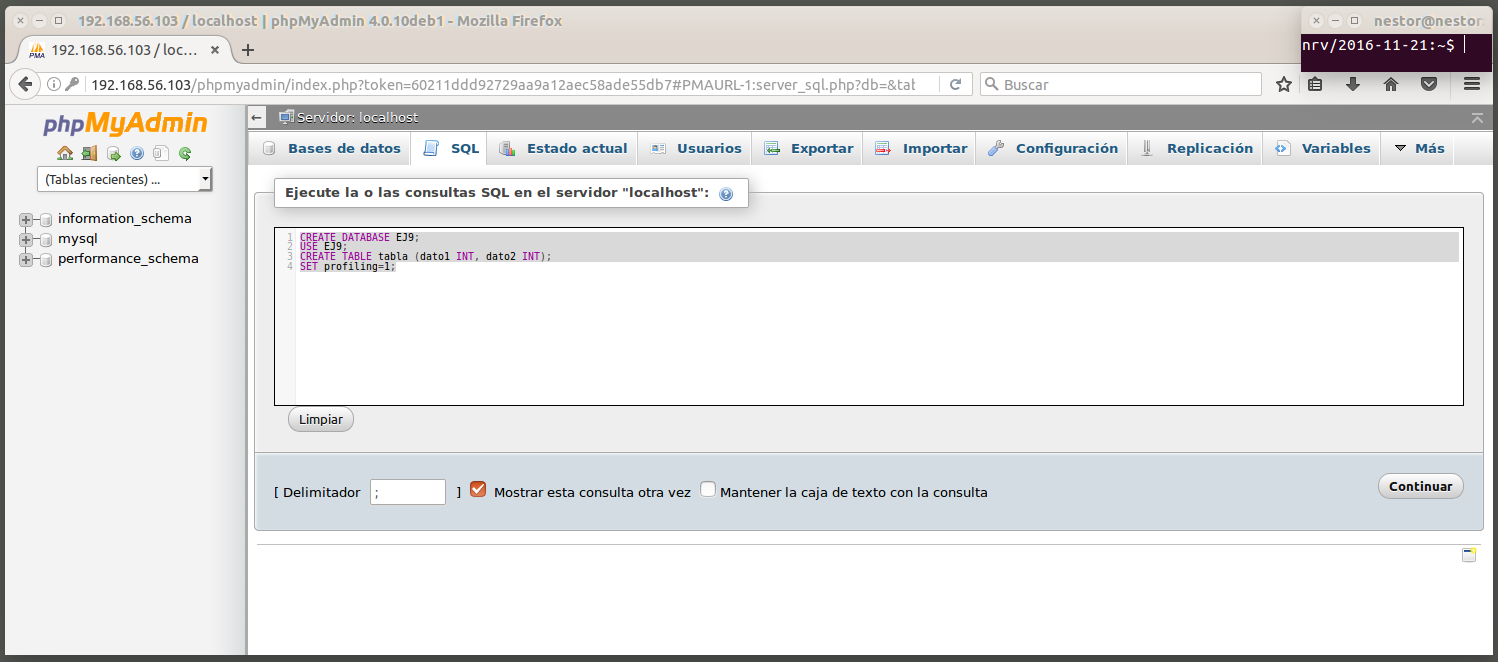
\includegraphics[width=\linewidth]{./Imagenes/9-2.png}
		\vspace{-0.5cm}
		\caption[Preparativos para el profiling.]{Preparativos para el profiling.}
		\label{9-2}
	\end{figure}
	
	Como podemos ver en la figura \ref{9-3}, la primera sentencia que ejecutamos ha creado la base de datos \textit{EJ9}, la segunda ha indicado que vamos a usar la base de datos \textit{EJ9}, la tercera sentencia sirve para crear una tabla llamada \textit{tabla} con dos columnas, \textit{dato1} que es un entero y \textit{dato2} que es un entero. La última sentencia es para habilitar el proceso de \textit{profiling}.
	
	\begin{figure}[H]
		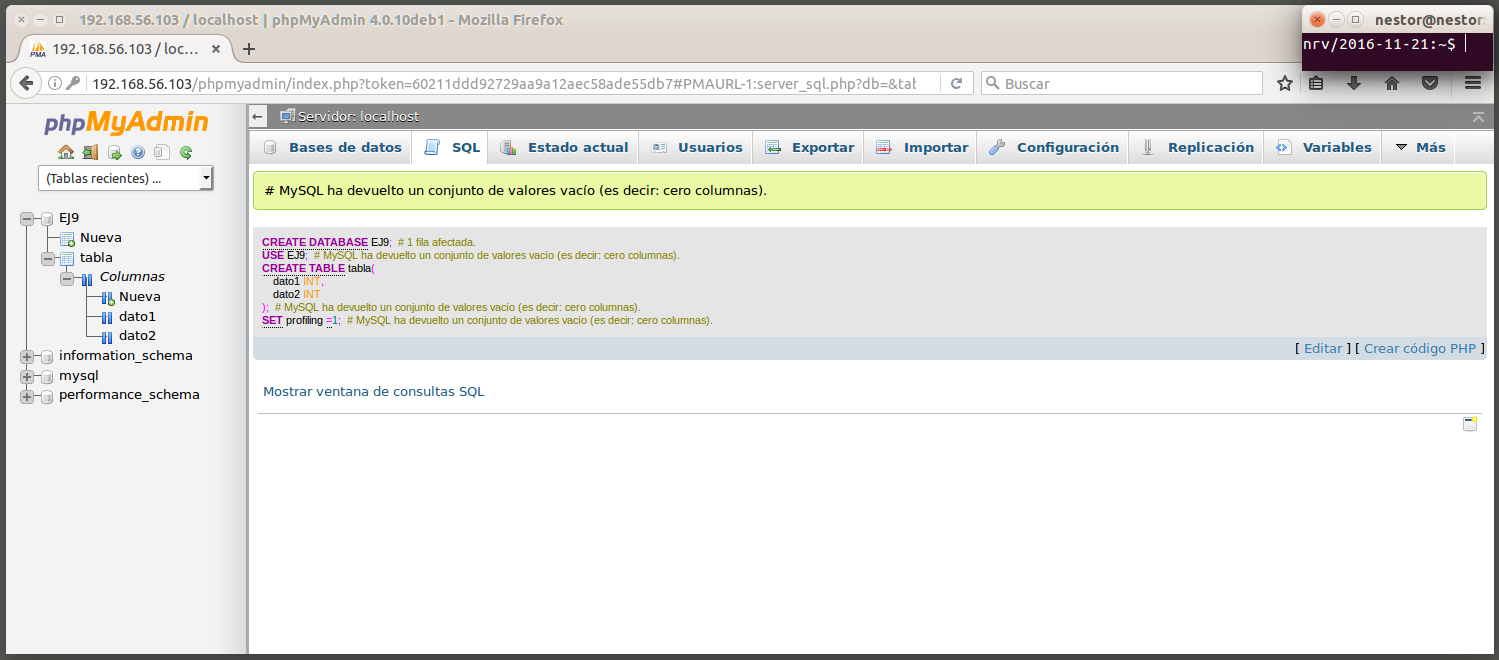
\includegraphics[width=\linewidth]{./Imagenes/9-3.png}
		\vspace{-0.5cm}
		\caption[Sentencias ejecutadas.]{Sentencias ejecutadas.}
		\label{9-3}
	\end{figure}
	
	Finalmente, insertamos algunas tuplas en la tabla, como podemos ver en la figura \ref{9-4}.
	
	\begin{figure}[H]
		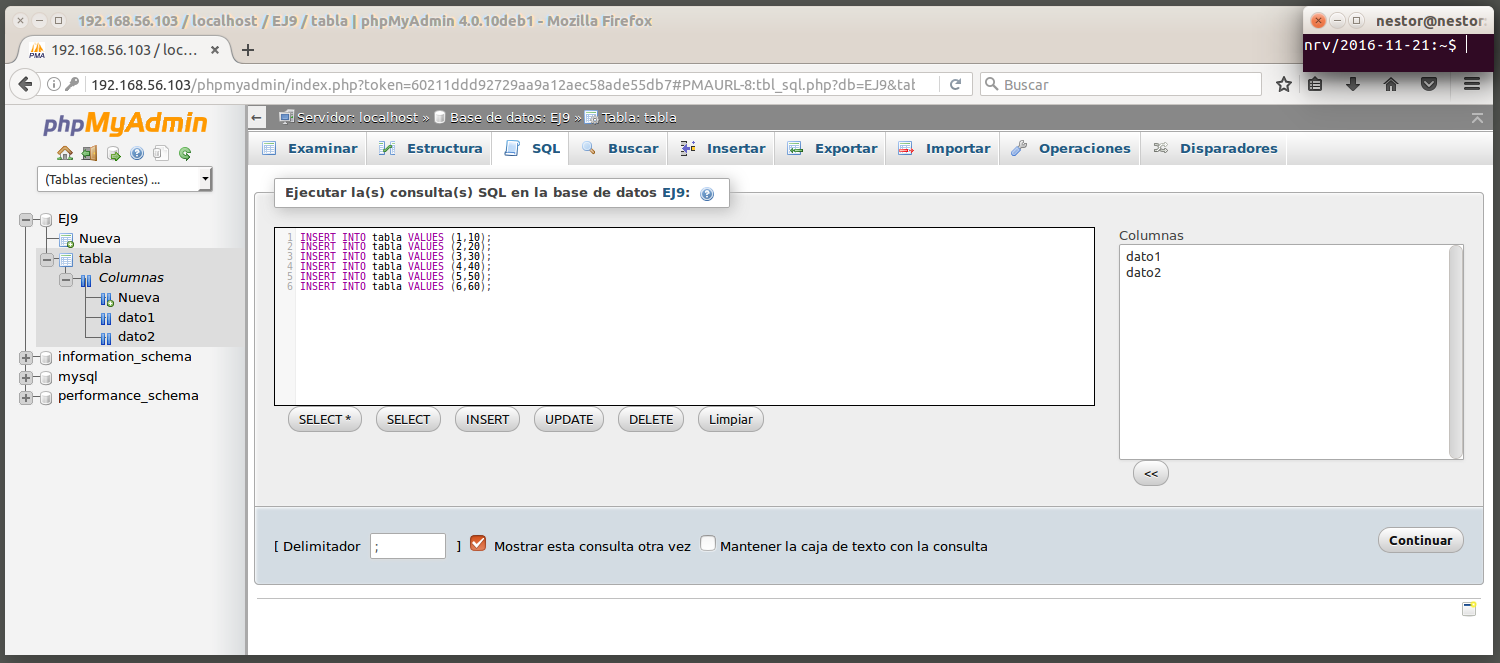
\includegraphics[width=\linewidth]{./Imagenes/9-4.png}
		\vspace{-0.5cm}
		\caption[Inserción de tuplas.]{Inserción de tuplas.}
		\label{9-4}
	\end{figure}
	
	Una vez tenemos las tuplas insertadas, realizamos una consulta. En mi caso, he recuperado todas las tuplas de la tabla ejecutando la sentencia \textit{SELECT * FROM tabla LIMIT 0,30}. El resultado lo podemos ver en la figura \ref{9-5}.
	
	\begin{figure}[H]
		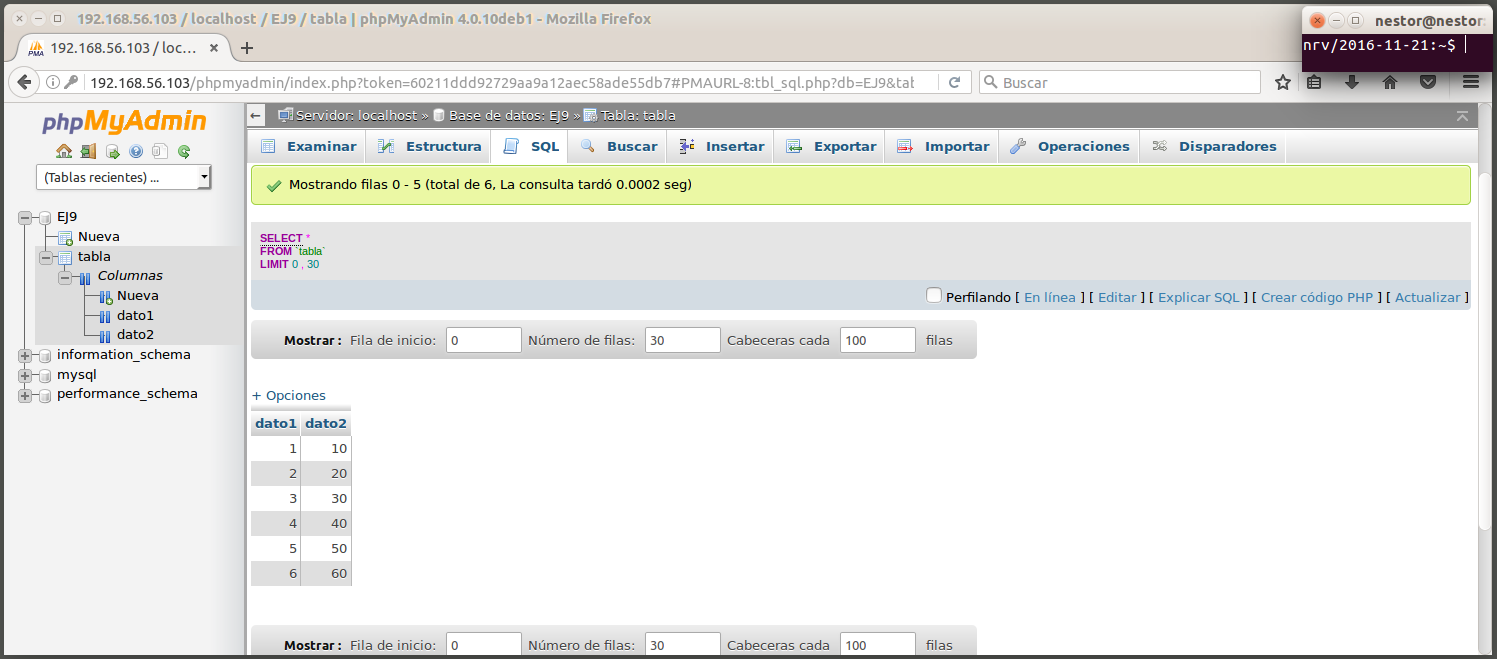
\includegraphics[width=\linewidth]{./Imagenes/9-5.png}
		\vspace{-0.5cm}
		\caption[Recuperación de todas las tuplas de la tabla.]{Recuperación de todas las tuplas de la tabla.}
		\label{9-5}
	\end{figure}
	
	Tras realizar la consulta, marcamos la opción \textit{Perfilando} y volvemos a ejecutar la consulta. En este caso, el resultado que obtenemos es el que podemos ver en la figura \ref{9-6}.
	
	\begin{figure}[H]
		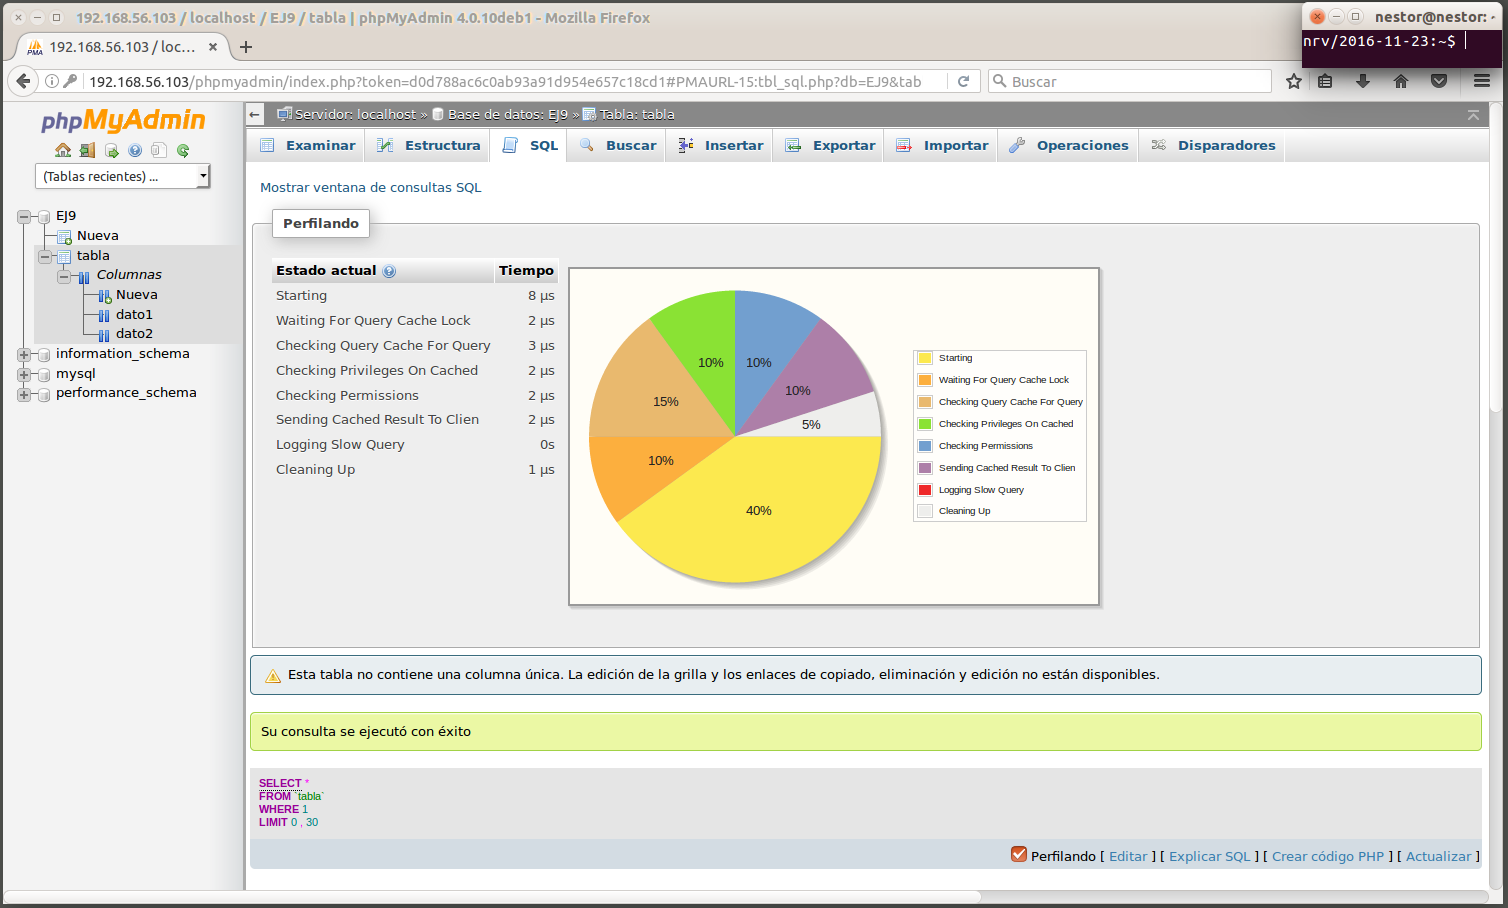
\includegraphics[width=\linewidth]{./Imagenes/9-6.png}
		\vspace{-0.5cm}
		\caption[Datos recogidos por el profiler tras la consulta.]{Datos recogidos por el profiler tras la consulta.}
		\label{9-6}
	\end{figure}
	
	El significado de las secciones que aparecen en los datos del profiler son \cite{profilermysql}:
	\begin{itemize}
		\item \textbf{Starting:} Tiempo empleado en comenzar.
		\item \textbf{Waiting For Query Cache Lock:} Tiempo esperando a conseguir un cerrojo sobre la cache de la consulta.
		\item \textbf{Checking Query Cache For Query:} Tiempo que tarda el servidor en comprobar si la consulta actual está presente en la caché de consultas.
		\item \textbf{Checking Privileges On Cached Query:} Tiempo que tarda el servidor en comprobar si el usuario tiene privilegios para acceder al resultado de una consulta ubicada en caché.
		\item \textbf{Checking Permissions:} Tiempo empleado en comprobar que los permisos son correctos.
		\item \textbf{Sending Cached Result To Client:} Tiempo que emplea el servidor en coger el resultado de una consulta en caché y enviarlo al cliente.
		\item \textbf{Logging Slow Query:} Tiempo empleado en loguearse en la cola lenta.
		\item \textbf{Cleaning up:} Tiempo empleado en limpiar los datos tras la consulta.
	\end{itemize}
	
	%%%%%%%%%%%%%%%%%%%%%%%%%%%%%%%%%%%%%%%%%%%%%%%%%%%%
	%%%%%%%%%%%%%%%%%%%% Cuestión Opcional 1 %%%%%%%%%%%
	%%%%%%%%%%%%%%%%%%%%%%%%%%%%%%%%%%%%%%%%%%%%%%%%%%%%
	\section[Cuestión opcional 1: Indique qué comandos ha utilizado para realizarlo así	como capturas de pantalla del proceso de reconstrucción del RAID.]{Cuestión opcional 1: Indique qué comandos ha utilizado para realizarlo así	como capturas de pantalla del proceso de reconstrucción del RAID.}
	
	Lo que he hecho ha sido seguir la misma idea que en la cuestión opcional 1 de la práctica 1 de esta asignatura. Al igual que en la práctica 1, me he basado en la información que podemos obtener de la Wiki de Linux \cite{raid}. Los pasos que he seguido son los siguientes:
	
	\begin{enumerate}
		\item Primero comprobamos que efectivamente tenemos dos RAID. Para ello ejecutamos el comando \textit{cat /proc/mdsatat} como se puede ver en la figura \ref{O1-1}. También se podría haber hecho con \textit{watch -n2 cat /proc/mdstat} pero como no se producen cambios en el fichero, no le sacamos partido a la utilidad \textit{watch}.
		\item A continuación, producimos un fallo por software en el RAID ejecutando el comando \textit{sudo mdadm -{-}manage -{-}set-faulty /dev/md0 /deb/sdb1} como podemos ver en la figura \ref{O1-2}.
		\item Retiramos el RAID en caliente ejecutando \textit{sudo mdadm /dev/md0 -r /dev/sdb1} y lo añadimos ejecutando \textit{sudo mdadm /dev/md0 -a /dev/sdb1}, como podemos ver en la figura \ref{O1-3}.
		\item Ahora si podemos sacarle partido a \textit{watch}. Para comprobar el proceso de recuperación del RAID ejecutamos \textit{watch -n2 cat /proc/mdstat}. De este modo, cada dos segundos se ejecutará \textit{cat /proc/mdstat}, proporcionándonos así una idea de como va el progreso, como se puede ver en la figura \ref{O1-4}.
		\item Tras un tiempo de recuperación, el RAID se ha recuperado correctamente y vuelve a estar en funcionamiento, como podemos ver en la figura \ref{O1-5}.
	\end{enumerate}
	
	\begin{figure}[H]
		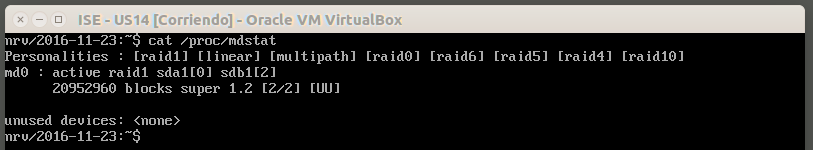
\includegraphics[width=\linewidth]{./Imagenes/O1-1.png}
		\vspace{-0.5cm}
		\caption[Comprobamos que tenemos dos RAID.]{Comprobamos que tenemos dos RAID.}
		\label{O1-1}
	\end{figure}
	
	\begin{figure}[H]
		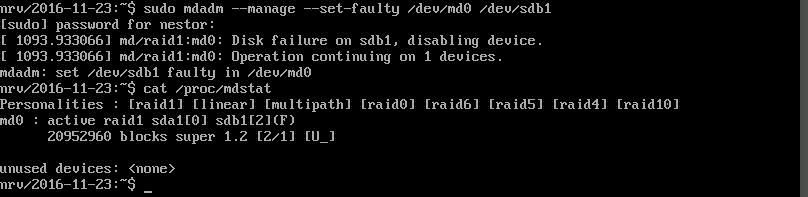
\includegraphics[width=\linewidth]{./Imagenes/O1-2.png}
		\vspace{-0.5cm}
		\caption[Provocamos un fallo software en el RAID.]{Provocamos un fallo software en el RAID.}
		\label{O1-2}
	\end{figure}
	
	\begin{figure}[H]
		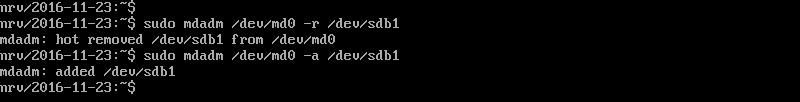
\includegraphics[width=\linewidth]{./Imagenes/O1-3.png}
		\vspace{-0.5cm}
		\caption[Quitamos en caliente y añadimos de nuevo el RAID.]{Quitamos en caliente y añadimos de nuevo el RAID.}
		\label{O1-3}
	\end{figure}
	
	\begin{figure}[H]
		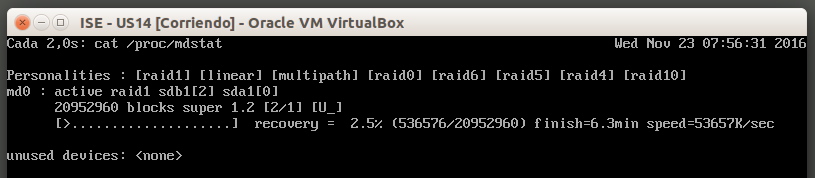
\includegraphics[width=\linewidth]{./Imagenes/O1-4.png}
		\vspace{-0.5cm}
		\caption[Observamos el proceso de recuperación con \textit{watch}.]{Observamos el proceso de recuperación con \textit{watch}.}
		\label{O1-4}
	\end{figure}
	
	\begin{figure}[H]
		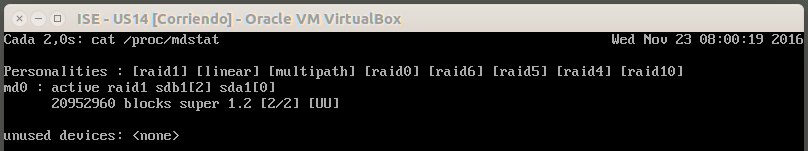
\includegraphics[width=\linewidth]{./Imagenes/O1-5.png}
		\vspace{-0.5cm}
		\caption[RAID completamente restaurado.]{RAID completamente restaurado.}
		\label{O1-5}
	\end{figure}
	
	%%%%%%%%%%%%%%%%%%%%%%%%%%%%%%%%%%%%%%%%%%%%%%%%%%%%
	%%%%%%%%%%%%%%%%%%%% Cuestión Opcional 2 %%%%%%%%%%%
	%%%%%%%%%%%%%%%%%%%%%%%%%%%%%%%%%%%%%%%%%%%%%%%%%%%%
	\section[Cuestión opcional 2: Instale Nagios en su sistema (el que prefiera) documentando el proceso y muestre el resultado de la monitorización de su sistema comentando qué aparece.]{Cuestión opcional 2: Instale Nagios en su sistema (el que prefiera) documentando el proceso y muestre el resultado de la monitorización de su sistema comentando qué aparece.}
	
	El proceso de instalación lo podemos ver en la página oficial de Nagios \cite{nagios}. Yo lo voy a hacer en CentOS. Los pasos a seguir son: 
	
	\begin{enumerate}
		\item El proceso de instalacion se hace desde el directorio \textit{/tmp}, así que ejecutamos \textit{cd /tmp} para irnos a dicha carpeta, como podemos ver en la figura \ref{O2-1}.
		\item Descargamos la última versión de \textit{Nagios}. Para ello ejecutamos el comando \textit{wget http://assets.nagios.com/downloads/nagiosxi/xi-latest.tar.gz}, como podemos ver en la figura \ref{O2-1}.
		\item Descomprimimos Nagios ejecutando \textit{tar xzf xi-latest.tar.gz}, como podemos ver en la figura \ref{O2-1}.
		\item Nos vamos a la carpeta que se ha creado ejecutando \textit{cd /tmp/nagiosxi}, como podemos ver en la figura \ref{O2-2}.
		\item Ejecutamos el script de instalación con el comando \textit{sudo ./fullinstalation}\footnote{Cuidado: este script cambia la contraseña del usuario root de MySQL a \textit{nagiosxi}}, como podemos ver en la figura \ref{O2-2}. Nos preguntara si queremos continuar, le decimos que sí pulsando la tecla \textit{y}.
	\end{enumerate}
	
	\begin{figure}[H]
		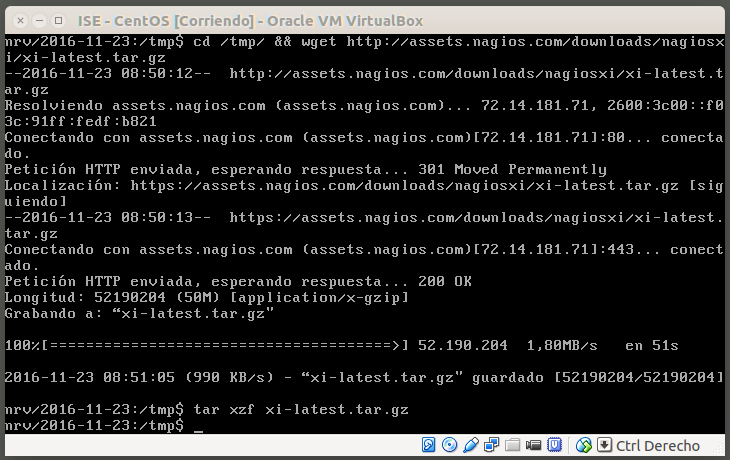
\includegraphics[width=\linewidth]{./Imagenes/O2-1.png}
		\vspace{-0.5cm}
		\caption[Proceso de descarga de Nagios y preparación para la instalación.]{Proceso de descarga de Nagios y preparación para la instalación.}
		\label{O2-1}
	\end{figure}
	
	\begin{figure}[H]
		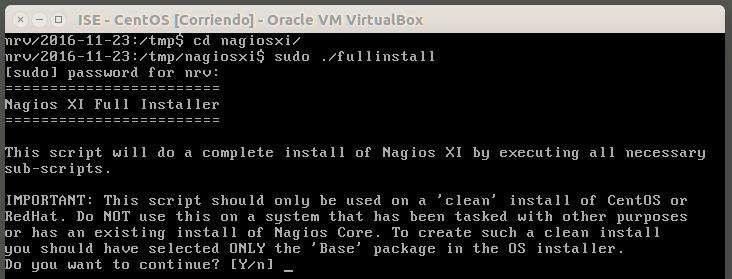
\includegraphics[width=\linewidth]{./Imagenes/O2-2.png}
		\vspace{-0.5cm}
		\caption[Proceso de instalación de Nagios.]{Proceso de instalación de Nagios.}
		\label{O2-2}
	\end{figure}
	
	Una vez hemos instalado Nagios, en el manual de instalación \cite{nagios} podemos ver que para acceder a Nagios desde mi máquina anfitriona debemos poner en el buscador \textit{http://IP/nagios}, donde \textit{IP} es la dirección del servidor al que nos queremos conectar. En mi caso, la dirección IP es \textit{192.168.56.101}, como podemos ver en la figura \ref{O2-conexion}. Tras introducir la dirección en el navegador, podemos ver que nos conectamos correctamente a Nagios, como se puede ver en la figura \ref{O2-conexion}.
	
	\begin{figure}[H]
		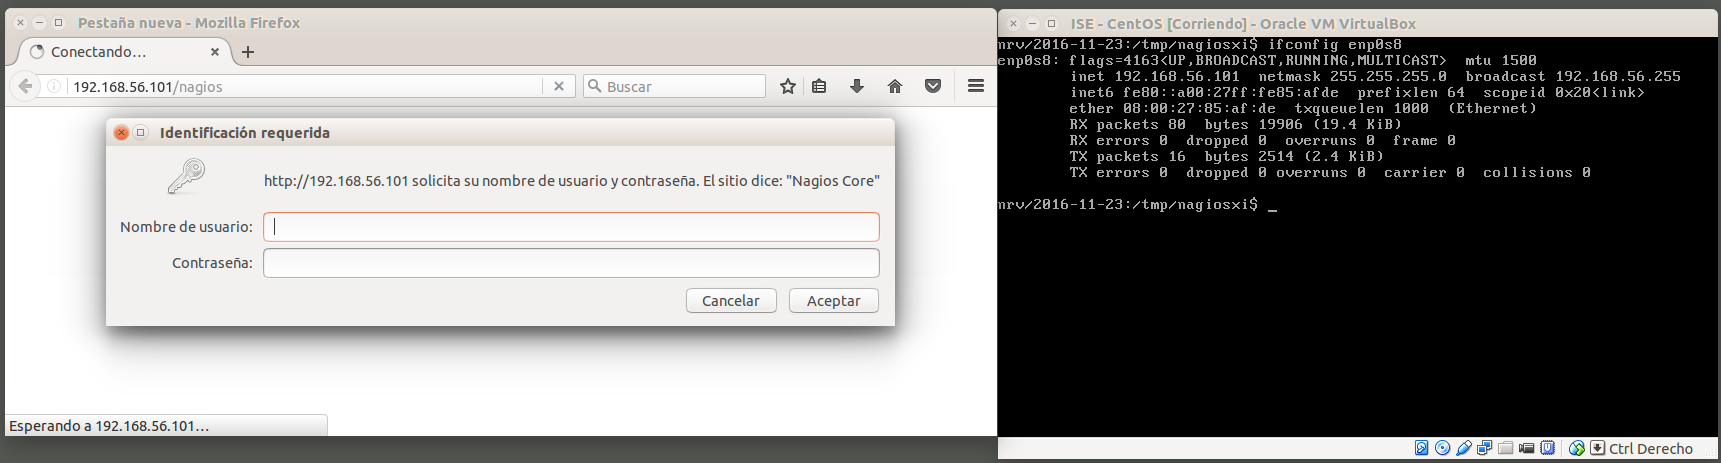
\includegraphics[width=\linewidth]{./Imagenes/O2-conexion.png}
		\vspace{-0.5cm}
		\caption[Conexión con Nagios (máquina conectadas en modo \textit{host-only}).]{Conexión con Nagios (máquina conectadas en modo \textit{host-only}).}
		\label{O2-conexion}
	\end{figure}
	
	Vemos que nos pide una contraseña. Para poder acceder debemos seguir los pasos que nos indica Nagios en su guía para configurar la interfaz web \cite{nagios2}. Debemos acceder a la dirección de nuestro servidor, como podemos ver en la figura \ref{O2-web1}. Una vez en dicha página, le damos a acceder y ahí configuramos nuestros datos, como podemos ver en la figura \ref{O2-web2}. A continuación, pulsamos \textit{install}.
	
	\begin{figure}[H]
		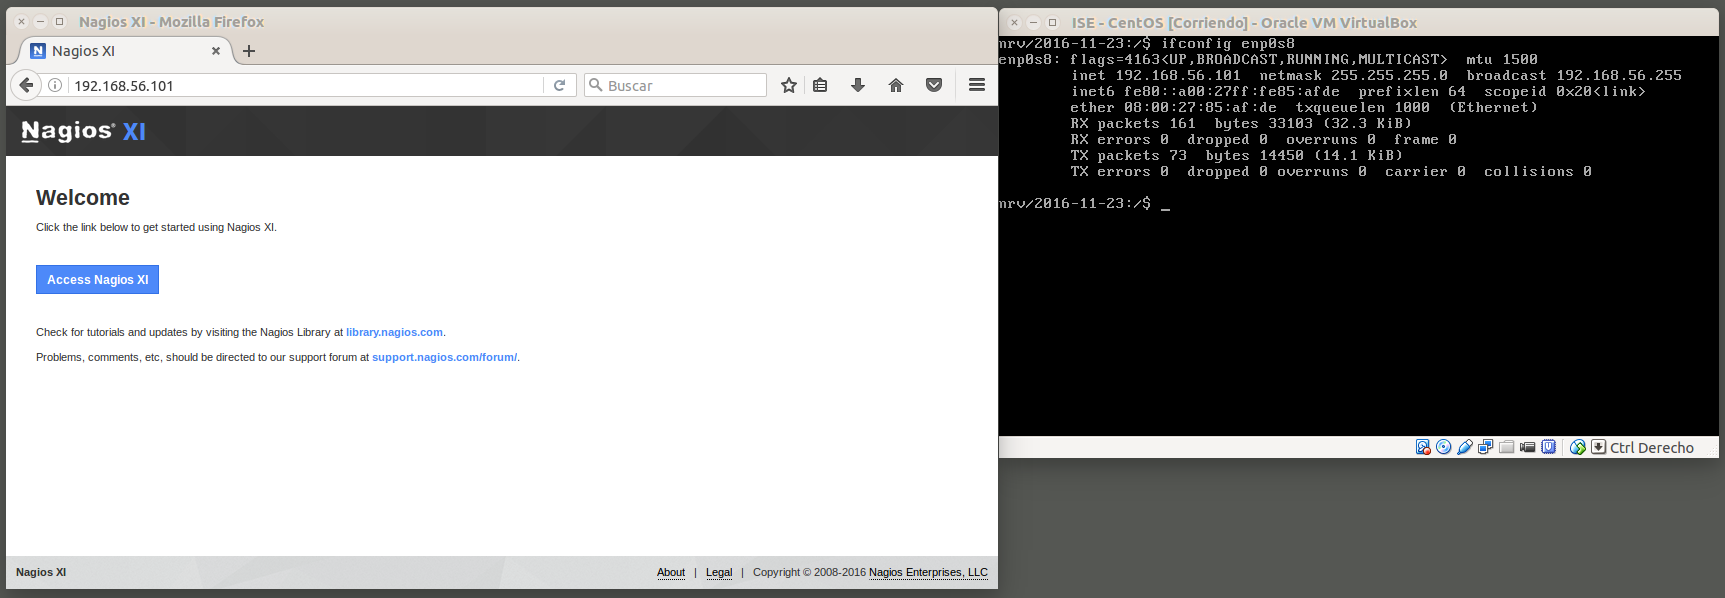
\includegraphics[width=\linewidth]{./Imagenes/O2-web1.png}
		\vspace{-0.5cm}
		\caption[Paso 1 de la configuración de la interfaz web (máquina conectadas en modo \textit{host-only}).]{Paso 1 de la configuración de la interfaz web (máquina conectadas en modo \textit{host-only}).}
		\label{O2-web1}
	\end{figure}
	
	\begin{figure}[H]
		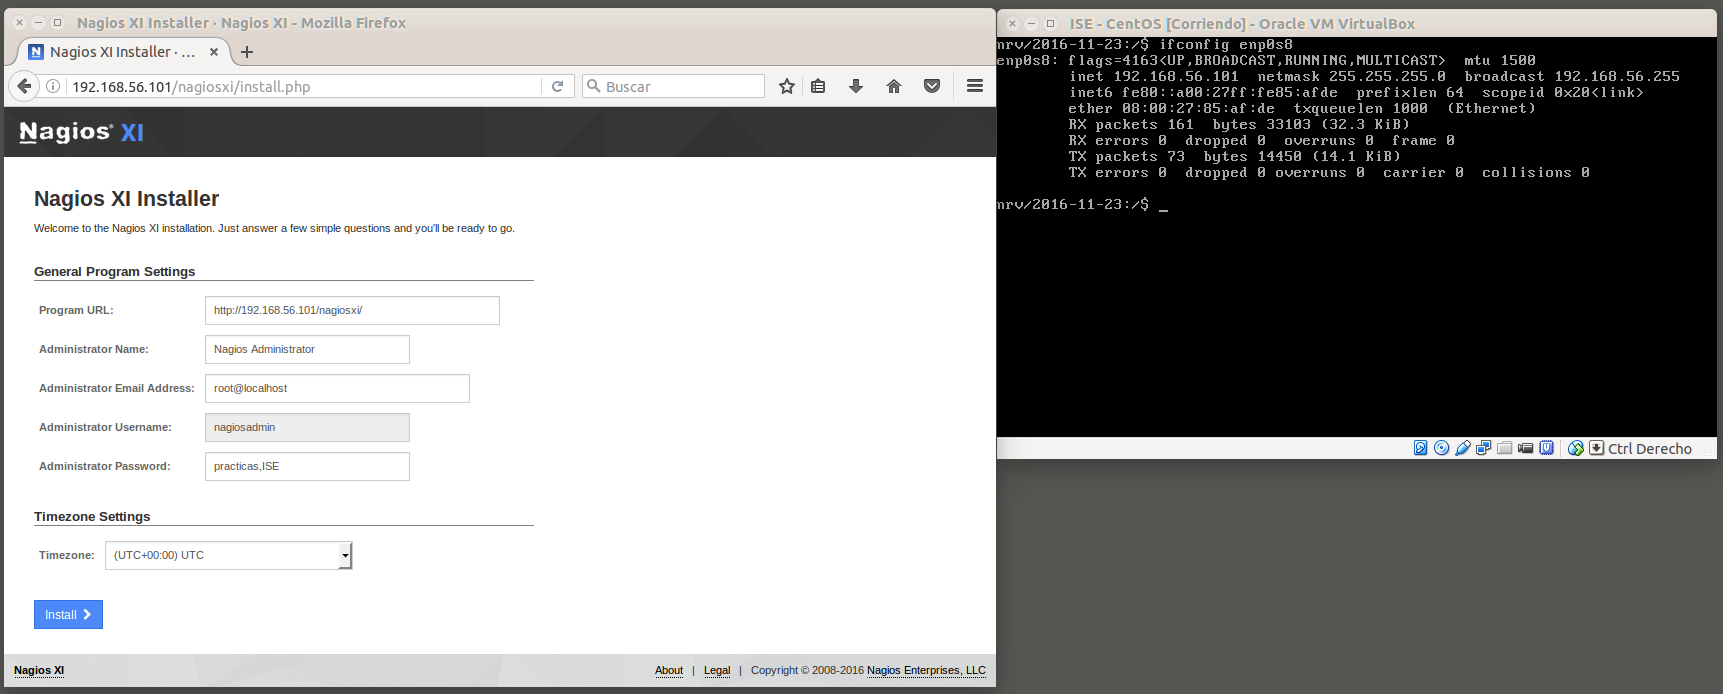
\includegraphics[width=\linewidth]{./Imagenes/O2-web2.png}
		\vspace{-0.5cm}
		\caption[Paso 2 de la configuración de la interfaz web (máquina conectadas en modo \textit{host-only}).]{Paso 2 de la configuración de la interfaz web (máquina conectadas en modo \textit{host-only}).}
		\label{O2-web2}
	\end{figure}
	
	Ahora si podemos acceder usando los datos que hemos introducido en el paso anterior (ver figura \ref{O2-web2}), como podemos ver en la figura \ref{O2-conexion2}.
	
	\begin{figure}[H]
		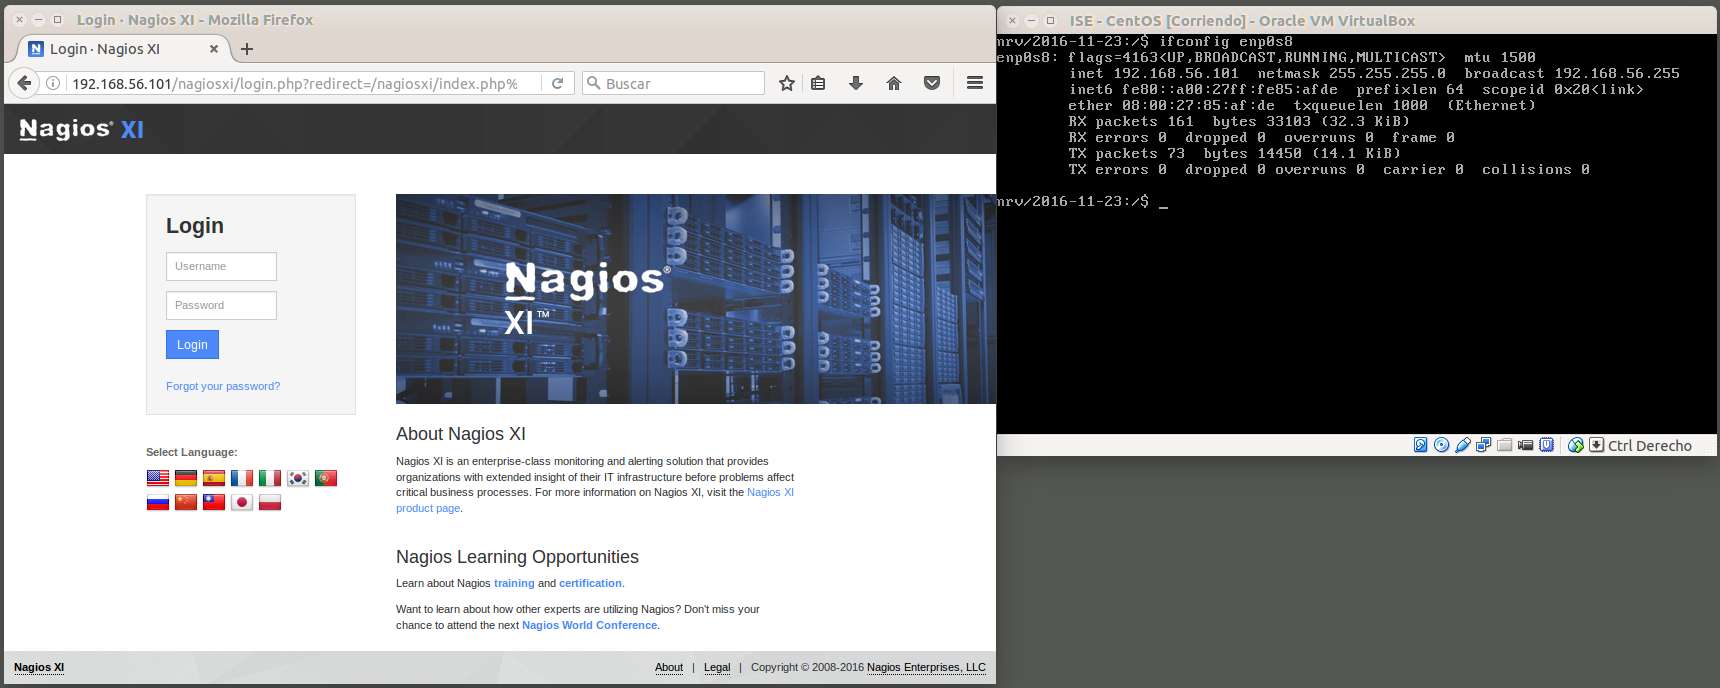
\includegraphics[width=\linewidth]{./Imagenes/O2-conexion2.png}
		\vspace{-0.5cm}
		\caption[Conexión con Nagios (máquina conectadas en modo \textit{host-only}).]{Conexión con Nagios (máquina conectadas en modo \textit{host-only}).}
		\label{O2-conexion2}
	\end{figure}
	
	Una vez hemos accedido a Nagios podemos ver que se pueden monitorizar diferentes parámetros. Como la mayoría de monitores, nos permite monitorizar el rendimiento de nuestro servidor, como podemos ver en la figura \ref{O2-rendimiento}. Una de las características que más me ha llamado la atención es la llamada \textit{Hypermap}. Esta opción nos muestra un mapa con el estado actual de los dispositivos de red (hosts), como podemos ver en la figura \ref{O2-hypermap}.
	
	\begin{figure}[H]
		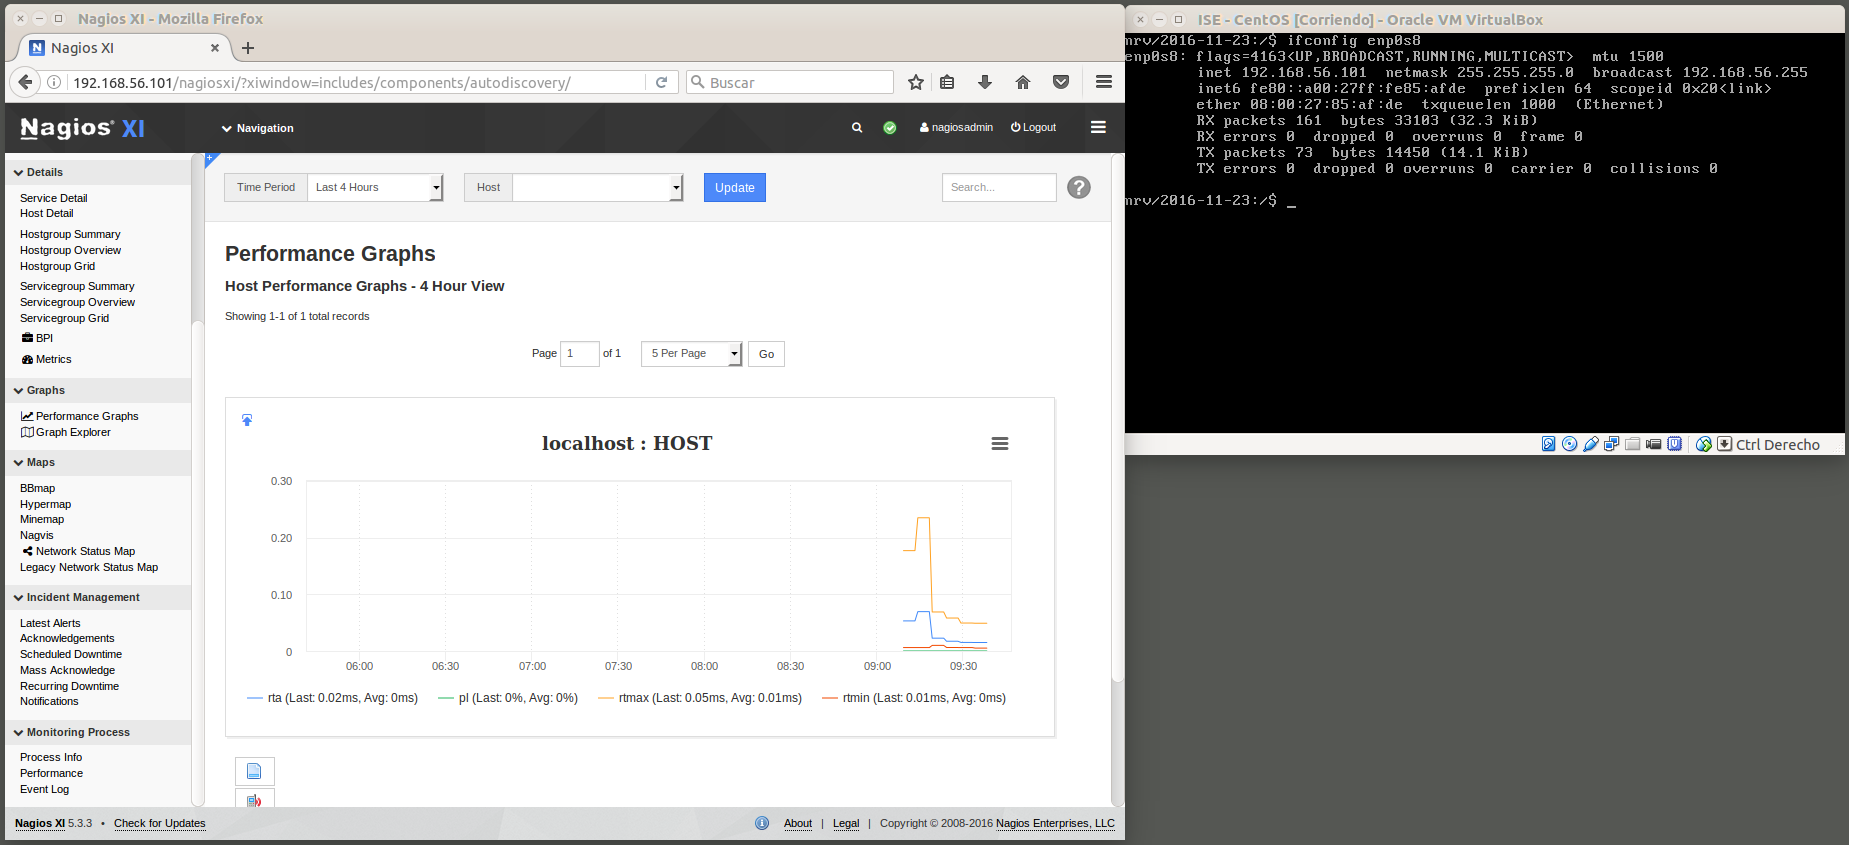
\includegraphics[width=\linewidth]{./Imagenes/O2-rendimiento.png}
		\vspace{-0.5cm}
		\caption[Monitorización del rendimiento con Nagios (máquina conectadas en modo \textit{host-only}).]{Monitorización del rendimiento con Nagios (máquina conectadas en modo \textit{host-only}).}
		\label{O2-rendimiento}
	\end{figure}
	
	\begin{figure}[H]
		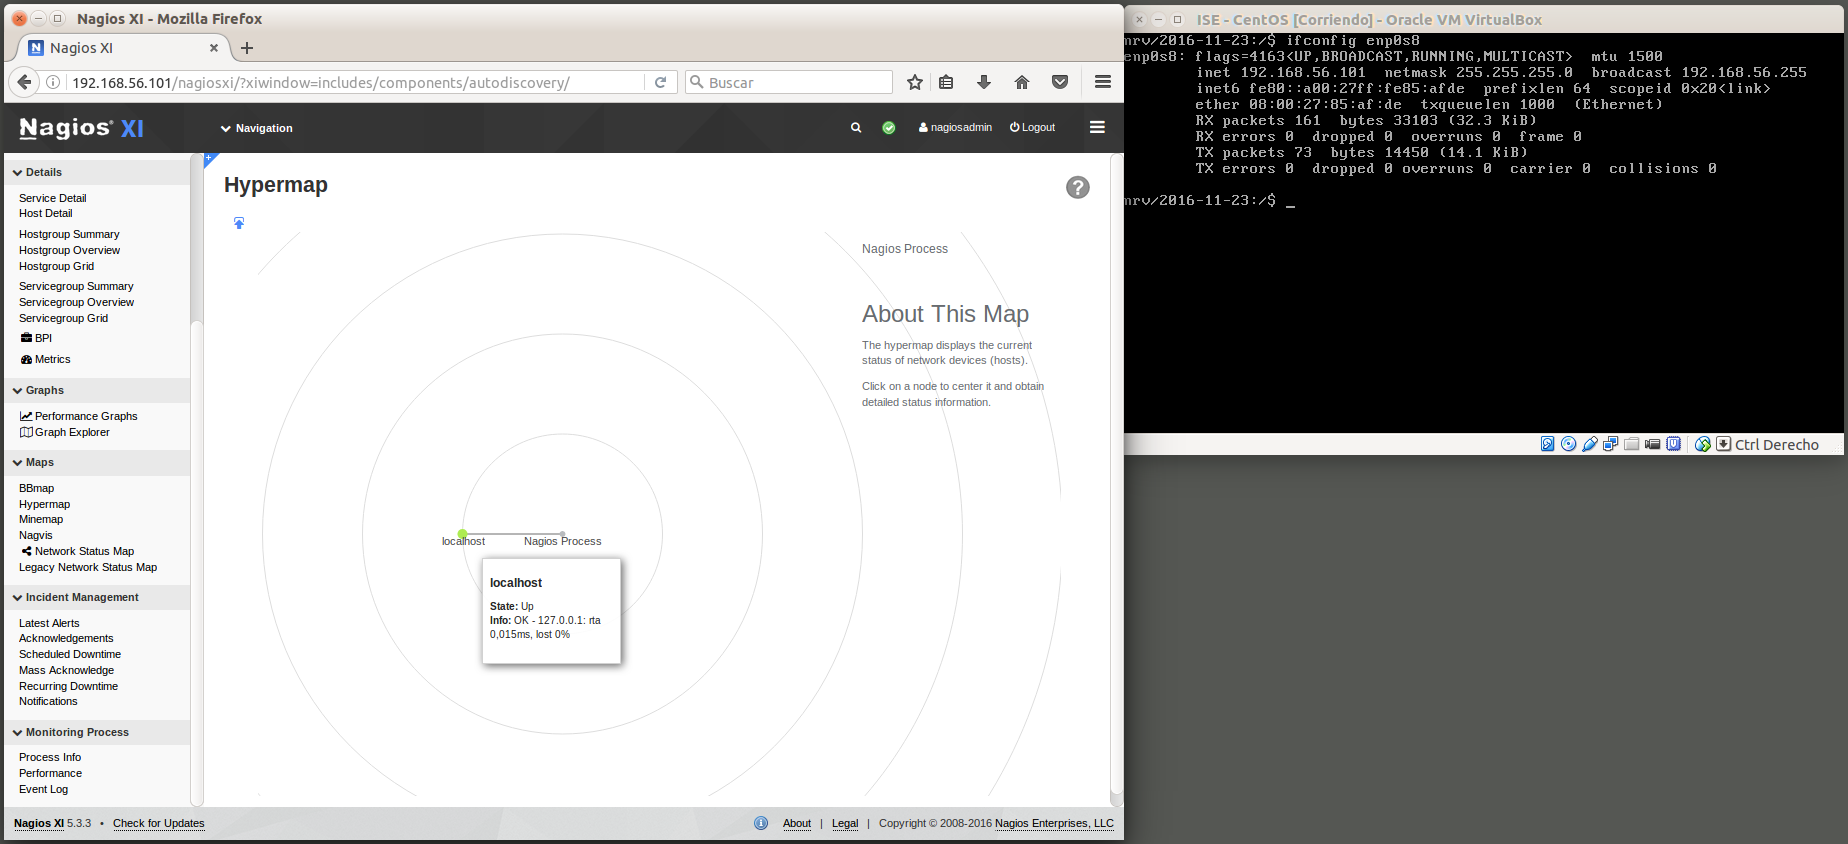
\includegraphics[width=\linewidth]{./Imagenes/O2-hypermap.png}
		\vspace{-0.5cm}
		\caption[Hypermap de mi servidor (máquina conectadas en modo \textit{host-only}).]{Hypermap de mi servidor  (máquina conectadas en modo \textit{host-only}).}
		\label{O2-hypermap}
	\end{figure}
	
	%%%%%%%%%%%%%%%%%%%%%%%%%%%%%%%%%%%%%%%%%%%%%%%%%%%%
	%%%%%%%%%%%%%%%%%%%% Cuestión Opcional 4 %%%%%%%%%%%
	%%%%%%%%%%%%%%%%%%%%%%%%%%%%%%%%%%%%%%%%%%%%%%%%%%%%
	\section[Cuestión opcional 4: Pruebe a instalar este monitor en alguno de sus tres sistemas. Realice capturas de pantalla del proceso de instalación y comente capturas de pantalla del programa en ejecución.]{Cuestión opcional 4: Pruebe a instalar este monitor en alguno de sus tres sistemas. Realice capturas de pantalla del proceso de instalación y comente capturas de pantalla del programa en ejecución.}
	
	Voy a instalar \textit{Zabbix} en Ubuntu Server siguiendo los pasos que nos indica Digital Ocean \cite{zabbix}. Los pasos a seguir para la instalación son: \label{pasos_zabbix}
	\begin{enumerate}
		\item \textit{Zabbix} se encuentra en los repositorios de Ubuntu, pero está desactualizado, por ello vamos a instalarlo desde los repositorios del programa. Para ello, editamos el fichero \textit{/etc/apt/sources.list} y añadimos las líneas: \\
		
		\# Zabbix Application PPA \\
		deb http://ppa.launchpad.net/tbfr/zabbix/ubuntu precise main \\
		deb-src http://ppa.launchpad.net/tbfr/zabbix/ubuntu precise main \\
		
		El archivo quedaría como podemos ver en la figura \ref{O4-1}.
		\item A continuación añadimos la clave del PPA para que \textit{apt} confíe en la fuente. Para ello ejecutamos: \textit{sudo apt-key adv -{-}keyserver keyserver.ubuntu.com -{-}recv-keys C407E17D5F76A32B}, como podemos ver en la figura \ref{O4-2}.
		\item Una vez hecho esto, actualizamos los repositorios con \textit{sudo apt-get update} e instalamos \textit{Zabbix} ejecutando \textit{zsudo apt-get install zabbix-server-mysql php5-mysql zabbix-frontend-php}, como podemos ver en la figura \ref{O4-2}.
	\end{enumerate}
	
	\begin{figure}[H]
		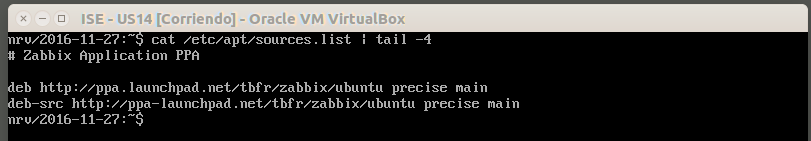
\includegraphics[width=\linewidth]{./Imagenes/O4-1.png}
		\vspace{-0.5cm}
		\caption[Archivo \textit{/etc/apt/sources.list}.]{Archivo \textit{/etc/apt/sources.list}.}
		\label{O4-1}
	\end{figure}
	
	\begin{figure}[H]
		\includegraphics[width=\linewidth]{./Imagenes/O4-2.png}
		\vspace{-0.5cm}
		\caption[Instalación de \textit{Zabbix}.]{Instalación de \textit{Zabbix}.}
		\label{O4-2}
	\end{figure}
	
	Los siguiente que debemos hacer es configurar el server de \textit{Zabbix}, para ello editamos el archivo \textit{/etc/zabbix/zabbix\_server.conf}, y cambiamos el valor de \textit{DBName}, \textit{DBUser} y\textit{DBPassword}. Dichos parámetros han quedado como podemos ver en la figura \ref{O4-3}.
	
	\begin{figure}[H]
		\includegraphics[width=\linewidth]{./Imagenes/O4-3.png}
		\vspace{-0.5cm}
		\caption[Configuración del servidor de \textit{Zabbix}.]{Configuración del servidor \textit{Zabbix}.}
		\label{O4-3}
	\end{figure}
	
	A continuación configuramos MySQL. Para ello seguimos los siguientes pasos:
	\begin{enumerate}
		\item Extramos los ficheros SQL del directorio \textit{cd /usr/share/zabbix-server-mysql/} ejecutando \textit{sudo gunzip *.gz}, como podemos ver en la figura \ref{O4-4}.
		\item Entramos a MySQL como usuarios root ejecutando \textit{mysql -u root -p}, como podemos ver en la figura \ref{O4-5}.
		\item Creamos un usuario para \textit{Zabbix} que coincida con los datos que escribimos en el fichero \textit{/etc/zabbix/zabbix\_server.conf} ejecutando \textit{create user `zabbix'@`localhost' identified by `practicas,ISE';}, como podemos ver en la figura \ref{O4-5}.
		\item Creamos una base de datos para \textit{Zabbix} ejecutando \textit{create database zabbix;}, como podemos ver en la figura \ref{O4-5}.
		\item Le damos permisos sobre dicha base de datos al usuario que hemos creado con anterioridad ejecutando \textit{grant all privileges on zabbix.* to `zabbix'@`localhost';}, como podemos ver en la figura \ref{O4-5}.
		\item Actualizamos los permisos ejecutando \textit{flush privileges;}, como podemos ver en la figura \ref{O4-5}.
		\item Salimos de MySQL ejecutando \textit{exit;}, como podemos ver en la figura \ref{O4-5}.
		\item Importamos los archivos que \textit{Zabbix} necesita para funcionar, para ello y como podemos ver en la figura \ref{O4-6}, ejecutamos:
			\begin{itemize}
				\item \textit{mysql -u zabbix -p zabbix $<$ schema.sql}
				\item \textit{mysql -u zabbix -p zabbix $<$ images.sql}
				\item \textit{mysql -u zabbix -p zabbix $<$ data.sql}
			\end{itemize}
	\end{enumerate}
	
	\begin{figure}[H]
		\includegraphics[width=\linewidth]{./Imagenes/O4-4.png}
		\vspace{-0.5cm}
		\caption[Extracción de ficheros SQL.]{Extracción de ficheros SQL.}
		\label{O4-4}
	\end{figure}
	
	\begin{figure}[H]
		\includegraphics[width=\linewidth]{./Imagenes/O4-5.png}
		\vspace{-0.5cm}
		\caption[Configuración de MySQL.]{Configuración de MySQL.}
		\label{O4-5}
	\end{figure}
	
	\begin{figure}[H]
		\includegraphics[width=\linewidth]{./Imagenes/O4-6.png}
		\vspace{-0.5cm}
		\caption[Importación de archivos necesarios para \textit{Zabbix}.]{Importación de archivos necesarios para \textit{Zabbix}.}
		\label{O4-6}
	\end{figure}
	
	Una vez hemos configurado MySQL, pasamos a la configuración de PHP. Para ello editamos el fichero \textit{/etc/php5/apache2/php.ini}. Buscamos y modificamos los siguientes parámetros para que queden como a continuación: 
	
	\begin{itemize}
		\item post\_max\_size = 16M
		\item max\_execution\_time = 300
		\item max\_input\_time = 300
		\item date.timezone = UTC
	\end{itemize}
	
	El resultado lo podemos ver en la figura \ref{O4-7}.
	
	\begin{figure}[H]
		\includegraphics[width=\linewidth]{./Imagenes/O4-7.png}
		\vspace{-0.5cm}
		\caption[Parámetros del archivo \textit{/etc/php5/apache2/php.ini} modificados.]{Parámetros del archivo \textit{/etc/php5/apache2/php.ini} modificados.}
		\label{O4-7}
	\end{figure}
	
	Copiamos el archivo de configuración de php específico de \textit{Zabbix} ejecutando \textit{sudo cp /usr/share/doc/zabbix-frontend-php/examples/zabbix.conf.php.example /etc/zabbix/zabbix.conf.php} para poder ejecutarlo y cambiar los parámetros que podemos ver a continuación para que queden de la siguiente manera:
	\begin{itemize}
		\item \$DB[``DATABASE''] = `zabbix';
		\item \$DB[``USER''] = `zabbix';
		\item \$DB[``PASSWORD''] = `practicas,ISE'
	\end{itemize}
	
	El resultado lo podemos ver en la figura \ref{O4-8}.
	
	\begin{figure}[H]
		\includegraphics[width=\linewidth]{./Imagenes/O4-8.png}
		\vspace{-0.5cm}
		\caption[Parámetros del archivo \textit{/etc/zabbix/zabbix.conf.php} modificados.]{Parámetros del archivo \textit{/etc/zabbix/zabbix.conf.php} modificados.}
		\label{O4-8}
	\end{figure}
	
	A continuación copiamos el archivo apache de \textit{Zabbix} en los archivos de configuración de apache ejecutando. Para ello ejecutamos:
	\begin{itemize}
		\item \textit{sudo cp /usr/share/doc/zabbix-frontend-php/examples/apache.conf /etc/apache2/\\conf-aviable/zabbix.conf}
		\item \textit{sudo cp /usr/share/doc/zabbix-frontend-php/examples/apache.conf /etc/apache2/\\conf-enable/zabbix.conf}
	\end{itemize}
	
	Nos aseguramos de que los alias están habilitados dentro de Apache ejecutando \textit{sudo a2enmod alias} y reiniciamos \textit{Apache} ejecutando \textit{sudo service apache2 restart}. Todo este proceso lo podemos ver en la figura \ref{O4-9}. Lo siguiente que tenemos que hacer es editar el fichero \textit{/etc/default/zabbix-server} y cambiar el valor de \textit{START} a ``yes'' e iniciamos \textit{Zabbix} ejecutando \textit{sudo service zabbix-server start} como podemos ver en la figura \ref{O4-10}.
	
	\begin{figure}[H]
		\includegraphics[width=\linewidth]{./Imagenes/O4-9.png}
		\vspace{-0.5cm}
		\caption[Configuración archivo apache de \textit{Zabbix}.]{Configuración archivo apache de \textit{Zabbix}.}
		\label{O4-9}
	\end{figure}
	
	\begin{figure}[H]
		\includegraphics[width=\linewidth]{./Imagenes/O4-10.png}
		\vspace{-0.5cm}
		\caption[Inicio de \textit{Zabbix}.]{Inicio de \textit{Zabbix}.}
		\label{O4-10}
	\end{figure}
	
	Ya está todo listo en el servidor, ahora debemos configurar el cliente. El cliente en mi caso va a ser mi máquina anfitriona. Debemos instalar el \textit{Agente de Zabbix}, para ello seguimos los 2 primeros pasos que realizamos en el servidor \ref{pasos_zabbix}, como podemos ver en la figura \ref{O4-11}. A continuación instalamos el \textit{Agente de Zabbix} ejecutando \textit{sudo apt-get install zabbix-agent}.
	
	\begin{figure}[H]
		\includegraphics[width=\linewidth]{./Imagenes/O4-11.png}
		\vspace{-0.5cm}
		\caption[Instalación del \textit{Agente de Zabbix}.]{Instalación del \textit{Agente de Zabbix}.}
		\label{O4-11}
	\end{figure}
	
	Una vez instalado, pasamos a modificar los archivos de configuración. El primero de ellos es \textit{/etc/zabbix/zabbix\_agentd.conf}. Como podemos ver en la figura \ref{O4-12} la dirección IP de mi servidor es \textit{192.168.56.103} así que en dicho archivo, en el parámetro \textit{Server} debemos poner dicha dirección, como se ve en la figura \ref{O4-12} y reiniciamos el servicio ejecutando \textit{sudo service zabbix-agent restart}.
	
	\begin{figure}[H]
		\includegraphics[width=\linewidth]{./Imagenes/O4-12.png}
		\vspace{-0.5cm}
		\caption[Dirección IP del servidor con \textit{Zabbix} instalado (máquinas conectadas en modo \textit{host-only}).]{Dirección IP del servidor con \textit{Zabbix} instalado (máquinas conectadas en modo \textit{host-only}).}
		\label{O4-12}
	\end{figure}
	
	Dentro del mismo fichero debemos editar el valor de \textit{Hostname} y poner el \textit{hostname} de la máquina cliente, \textit{nestor} en mi caso, y reiniciamos el servicio, como podemos ver en la figura \ref{O4-13}
	
	\begin{figure}[H]
		\includegraphics[width=\linewidth]{./Imagenes/O4-13.png}
		\vspace{-0.5cm}
		\caption[Parámetro \textit{hostname}.]{Parámetro \textit{hostname}.}
		\label{O4-13}
	\end{figure}
	
	Finalmente, para acceder al servicio debemos escribir en la barra del navegador la dirección IP de nuestro servidor seguido de \textit{/zabbix}, como podemos ver en la figura \ref{O4-14}. Por defecto, el usuario y contraseña para entrar son \textit{admin} y \textit{zabbix} respectivamente.
	
	\begin{figure}[H]
		\includegraphics[width=\linewidth]{./Imagenes/O4-14.png}
		\vspace{-0.5cm}
		\caption[\textit{Zabbix} en funcionamiento.]{\textit{Zabbix} en funcionamiento}
		\label{O4-14}
	\end{figure}
	
	Una vez hemos entrado, nos vamos a la pestaña \textit{Configuration} y dentro de dicha pestaña elegimos la de \textit{Hosts}, como podemos ver la figura \ref{O4-15}. Una vez aquí, pinchamos sobre \textit{Zabbix Server}.
	
	\begin{figure}[H]
		\includegraphics[width=\linewidth]{./Imagenes/O4-15.png}
		\vspace{-0.5cm}
		\caption[Host disponibles.]{Host disponibles.}
		\label{O4-15}
	\end{figure}
	
	Dentro del servidor de \textit{Zabbix}, al final de todo, en la sección de \textit{Status} elegimos \textit{Monitored}, como podemos ver en la figura \ref{O4-16}.
	
	\begin{figure}[H]
		\includegraphics[width=\linewidth]{./Imagenes/O4-16.png}
		\vspace{-0.5cm}
		\caption[Cambio del estado del servidor.]{Cambio del estado del servidor.}
		\label{O4-16}
	\end{figure}
	
	Tras unos instantes, podemos ver que en la pestaña \textit{Last data} dentro de \textit{Monitorig} los distintos hosts que se pueden modificar. Dentro de nuestro servidor \textit{Zabbix}, podemos ver una gran cantidad de parámetros monitorizados. Parte de ellos los podemos ver en la figura \ref{O4-17}.
	
	\begin{figure}[H]
		\includegraphics[width=\linewidth]{./Imagenes/O4-17.png}
		\vspace{-0.5cm}
		\caption[Parámetros monitorizados.]{Parámetros monitorizados.}
		\label{O4-17}
	\end{figure}
	
	Uno de los parámetros que podemos ver es el número de valores procesados por el servidor \textit{Zabbix} por segundo. Podemos ver una gráfica sobre la información recogida de dicho parámetro en la figura \ref{O4-18}. En dicha gráfica podemos ver que no hay mucha actividad en el servidor. El servidor se ha puesto en marcha a las 23:14 y la gráfica llega hasta las 23:36. En este periodo el valor se mantiene ``constante'' en un valor algo superior a 0.38. Podemos ver que hay dos picos a las 23:18 y 23:28 con un valor cercano a 0.42 valores procesados por el servidor \textit{Zabbix} por segundo.
	
	\begin{figure}[H]
		\includegraphics[width=\linewidth]{./Imagenes/O4-18.png}
		\vspace{-0.5cm}
		\caption[Valores procesados por el servidor \textit{Zabbix} por segundo.]{Valores procesados por el servidor \textit{Zabbix} por segundo.}
		\label{O4-18}
	\end{figure}
	
	%%%%%%%%%%%%%%%%%%%%%%%%%%%%%%%%%%%%%%%%%%%%%%%%%%%%
	%%%%%%%%%%%%%%%%%%%% Cuestión Opcional 5 %%%%%%%%%%%
	%%%%%%%%%%%%%%%%%%%%%%%%%%%%%%%%%%%%%%%%%%%%%%%%%%%%
	\section[Cuestión opcional 5: Pruebe a instalar este monitor en alguno de sus tres sistemas. Realice capturas de pantalla del proceso de instalación y comente capturas de pantalla del programa en ejecución.]{Cuestión opcional 5: Pruebe a instalar este monitor en alguno de sus tres sistemas. Realice capturas de pantalla del proceso de instalación y comente capturas de pantalla del programa en ejecución.}
	
	La instalación voy a hacerla en CentOS. Siguiendo la documentación de la página oficial de Cacti \cite{cacti}, debemos ejecutar el comando \textit{sudo yum install cacti}, como podemos ver en la figura \ref{O5-instalacion}.
	
	\begin{figure}[H]
		\includegraphics[width=\linewidth]{./Imagenes/O5-instalacion.png}
		\vspace{-0.5cm}
		\caption[Instalación de Cacti.]{Instalación de Cacti.}
		\label{O5-instalacion}
	\end{figure}
	
	Cómo podemos ver en la  documentación de Cacti \cite{cacti_paquetes}, para su correcto funcionamiento necesitamos que los siguientes paquetes esté instalados: 
	\begin{itemize}
		\item httpd
		\item php
		\item php-mysql
		\item php-snmp
		\item mysql
		\item mysql-server \footnote{Dado que lo estoy haciendo en CentOS, yo uso \textit{mariadb}, como ya explique en prácticas anteriores.}
		\item net-snmp
	\end{itemize}
	
	La mayoría de estos paquetes los hemos ido instalando a lo largo de las prácticas y los que no, ya vienen instalados por defecto en CentOS. Una ves está todo instalado, iniciamos los servicios. Como podemos ver en la figura \ref{O5-1}, ejecutamos:
	\begin{itemize}
		\item systemctl start httpd.service
		\item systemctl start mariadb.service
		\item systemctl start snmpd.service
	\end{itemize}
	
	\begin{figure}[H]
		\includegraphics[width=\linewidth]{./Imagenes/O5-1.png}
		\vspace{-0.5cm}
		\caption[Iniciamos los servicios.]{Iniciamos los servicios.}
		\label{O5-1}
	\end{figure}
	
	A continuación, debemos configurar las bases de datos de MySQL (MariaDB en mi caso) tal y cómo nos indican en la documentación de Cacti \cite{cacti_mysql}. Lo primero que hacemos es entrar a MariaDB ejecutando \textit{mysql -u root -p}. Una vez dentro, como podemos ver en la figura \ref{O5-2}, realizamos los siguientes pasos:
	\begin{enumerate}
		\item Creamos la base de datos para \textit{Cacti} ejecutando \textit{create database cacti;}
		\item Concedemos permisos sobre esa base de datos y creamos un usuario ejecutando \textit{grant all on cacti.* to `cacti'@`localhost' identified by `practicas,ISE';}
		\item Actualizamos los permisos ejecutando \textit{flush privileges;}
		\item Salimos de MariaDB ejecutando \textit{exit;}
	\end{enumerate}
	
	\begin{figure}[H]
		\includegraphics[width=\linewidth]{./Imagenes/O5-2.png}
		\vspace{-0.5cm}
		\caption[Creación base de datos para \textit{Cacti}.]{Creación base de datos para \textit{Cacti}.}
		\label{O5-2}
	\end{figure}
	
	Importamos las tablas de \textit{Cacti} ejecutando \textit{mysql -u cacti -p cacti $<$ /usr/share/doc/cacti-0.8.8b/cacti.sql}, como podemos ver en la figura \ref{O5-3}.
	
	\begin{figure}[H]
		\includegraphics[width=\linewidth]{./Imagenes/O5-3.png}
		\vspace{-0.5cm}
		\caption[Importación de las tablas para \textit{Cacti}.]{Importación de las tablas para \textit{Cacti}.}
		\label{O5-3}
	\end{figure}
	
	A continuación, debemos editar el archivo \textit{/etc/cacti/db.php} y cambiar los parámetros que podemos ver a continuación para que queden de la siguiente manera:
	\begin{itemize}
		\item \$database\_type = ``mysql'';
		\item \$database\_default = ``cacti'';
		\item \$database\_hostname = ``localhost'';
		\item \$database\_username = ``cacti'';
		\item \$database\_password = ``practicas,ISE'';
	\end{itemize}
	
	El resultado de modificar dicho archivo lo podemos ver en la figura \ref{O5-4}.
	
	\begin{figure}[H]
		\includegraphics[width=\linewidth]{./Imagenes/O5-4.png}
		\vspace{-0.5cm}
		\caption[Parámetros modificados.]{Parámetros modificados.}
		\label{O5-4}
	\end{figure}
	
	Asignamos los permisos a \textit{/usr/share/cacti/rra} y a \textit{/usr/share/cacti/log} correctamente. Para ello, como podemos ver en la figura \ref{O5-5} ejecutamos:
	\begin{itemize}
		\item \textit{chown -R cacti /usr/share/cacti/rra/}
		\item \textit{chown -R cacti /usr/share/cacti/log/}
	\end{itemize}
	
	\begin{figure}[H]
		\includegraphics[width=\linewidth]{./Imagenes/O5-5.png}
		\vspace{-0.5cm}
		\caption[Permisos modificados.]{Permisos modificados.}
		\label{O5-5}
	\end{figure}
	
	A continuación debemos editar el fichero de configuración de \textit{Apache} en función de la versión que tenemos. En CentOS, tengo la versión 2.4.6 \footnote{Para ver la versión que tenemos instalada debemos ejecutar \textit{httpd -v}}, por lo tanto debemos modificar la parte correspondiente a versiones 2.4 de \textit{Apache}. Debemos permitir conexiones desde el exterior de nuestro servidor, por eso cambiamos la línea que hay debajo de la línea \textit{\# httpd 2.4} por \textit{Requiere all granted}. Una vez hecho el cambio, reiniciamos \textit{Apache} ejecutando \textit{sudo systemctl restart httpd.service}. Por último editamos nuestro fichero \textit{crontab} ejecutando \textit{*/5 * * * * cacti php /usr/share/cacti/poller.php $>$ /dev/null 2$>$\&1}. Este proceso lo podemos ver en la figura \ref{O5-6}.
	
	\begin{figure}[H]
		\includegraphics[width=\linewidth]{./Imagenes/O5-6.png}
		\vspace{-0.5cm}
		\caption[Archivo de configuración de \textit{Apache} y archivo \textit{crontab} modificados.]{Archivo de configuración de \textit{Apache} y archivo \textit{crontab} modificados.}
		\label{O5-6}
	\end{figure}
	
	Finalmente, para acceder a \textit{cacti} desde nuestra máquina anfitriona, debemos introducir la dirección IP de nuestro servidor seguido de \textit{/cacti}. En mi caso, la dirección IP de mi servidor es \textit{192.168.56.101} (máquinas conectadas en modo \textit{host-only}), así que debemos escribir \textit{192.168.56.101/cacti}, como podemos ver en la figura \ref{O5-7}.
	
	\begin{figure}[H]
		\includegraphics[width=\linewidth]{./Imagenes/O5-7.png}
		\vspace{-0.5cm}
		\caption[\textit{Cacti} en funcionamiento.]{\textit{Cacti} en funcionamiento.}
		\label{O5-7}
	\end{figure}
	
	Desde el navegador, debemos instalar cacti. Para ello, pulsamos el botón de \textit{Next}. En la pantalla que podemos ver en la figura \ref{O5-8}, elegimos \textit{New Install} y le damos a \textit{Next}. En la siguiente ventana, que podemos ver en la figura \ref{O5-9}, le damos a \textit{Finish}. Finalmente, podemos ver la pantalla de inicio de sesión, como se ve en la figura \ref{O5-10}.
	
	\begin{figure}[H]
		\includegraphics[width=\linewidth]{./Imagenes/O5-8.png}
		\vspace{-0.5cm}
		\caption[Instalación nueva.]{Instalación nueva.}
		\label{O5-8}
	\end{figure}
	
	\begin{figure}[H]
		\includegraphics[width=\linewidth]{./Imagenes/O5-9.png}
		\vspace{-0.5cm}
		\caption[Finalización de la instalación.]{Finalización de la instalación.}
		\label{O5-9}
	\end{figure}
	
	\begin{figure}[H]
		\includegraphics[width=\linewidth]{./Imagenes/O5-10.png}
		\vspace{-0.5cm}
		\caption[Instalación de \textit{Cacti} completada.]{Instalación de \textit{Cacti} completada.}
		\label{O5-10}
	\end{figure}
	
	En la página que vemos en la figura \ref{O5-10} accedemos poniendo como usuario y contraseña \textit{admin} y \textit{admin} correspondientemente. Una vez introducida los datos, se nos obliga a cambiar la contraseña, como podemos ver en la figura \ref{O5-11}. En mi caso, he introducido la de siempre: \textit{practicas,ISE}.
	
	\begin{figure}[H]
		\includegraphics[width=\linewidth]{./Imagenes/O5-11.png}
		\vspace{-0.5cm}
		\caption[Cambio forzado de contraseña.]{Cambio forzado de contraseña.}
		\label{O5-11}
	\end{figure}
	
	Una vez instalado hemos instalado \textit{Cacti}, seleccionamos el gráfico que queremos añadir al árbol de gráfico y lo añadimos, tal y cómo podemos ver en la figura \ref{O5-12}. Para ver el gráfico, pinchamos sobre la opción de \textit{graphs} que podemos ver en la parte superior de \textit{cacti}. Podemos ver los datos en la figura \ref{O5-13}.
	
	\begin{figure}[H]
		\includegraphics[width=\linewidth]{./Imagenes/O5-12.png}
		\vspace{-0.5cm}
		\caption[Añadimos el gráfico al árbol.]{Añadimos el gráfico al árbol.}
		\label{O5-12}
	\end{figure}
	
	\begin{figure}[H]
		\includegraphics[width=\linewidth]{./Imagenes/O5-13.png}
		\vspace{-0.5cm}
		\caption[Datos recogidos.]{Datos recogidos.}
		\label{O5-13}
	\end{figure}
	
	Los gráficos que podemos ver en la figura \ref{O5-13} representan la carga media del servidor y número de usuarios identificados en el sistema. En ambos casos parece que no hay datos ya que no se ha producido nada en el servidor en el intervalo te tiempo seleccionado.
	
	%%%%%%%%%%%%%%%%%%%%%%%%%%%%%%%%%%%%%%%%%%%%%%%%%%%%
	%%%%%%%%%%%%%%%%%%%% Cuestión Opcional 6 %%%%%%%%%%%
	%%%%%%%%%%%%%%%%%%%%%%%%%%%%%%%%%%%%%%%%%%%%%%%%%%%%
	\section[Cuestión opcional 6: Instale el monitor. Muestre y comente algunas capturas de pantalla.]{Cuestión opcional 6: Instale el monitor. Muestre y comente algunas capturas de pantalla.}
	
	Para instalar \textit{AWStats} ejecutamos \textit{sudo apt-get install awstats}. Una vez lo hemos instalado, como podemos ver en la \textit{Community Help Wiki} de Ubuntu \cite{awstats_instalacion}, si quisiésemos monitorizar varios dominios, debemos crear un archivo de configuración para cada uno. En mi caso sólo voy a monitorizar el localhost, así que con modificar el archivo que tenemos es suficiente. Debemos editar el fichero cambiando los parámetros que vemos a continuación para que reflejen la información correcta. En mi caso, el valor de los parámetros es el siguiente: 
	\begin{itemize}
		\item LogFile=``/var/log/apache2/access.log''
		\item SiteDomain=``localhost''
		\item HostAliases=``localhost 127.0.0.1''
	\end{itemize}
	
	El resultado de la modificación de dicho archivo lo podemos ver en la figura \ref{O6-1}. Una vez editado el fichero, creamos las estadísticas iniciales para \textit{AWStats}. Para ello ejecutamos \textit{sudo /usr/lib/cgi-bin/awstats.pl -config=localhost -update}, tal y como se puede ver en la figura \ref{O6-1}.
	
	\begin{figure}[H]
		\includegraphics[width=\linewidth]{./Imagenes/O6-1.png}
		\vspace{-0.5cm}
		\caption[Configuración de \textit{AWStats}.]{Configuración de \textit{AWStats}.}
		\label{O6-1}
	\end{figure}
	
	Una vez hemos configurado \textit{AWStats}, pasamos a configurar \textit{Apache}. Lo primero que debemos hacer indicarle a \textit{Apache} que use \textit{mod\_cgi} ejecutando \textit{sudo a2enmod cgi}. Dado que no tenemos ningún \textit{Host Virtual}, creamos el archivo \textit{/etc/apache2/sites-available/default} y añadimos las líneas que podemos ver en la figura \ref{O6-2}. También debemos añadir estás líneas al fichero \textit{/etc/apache2/sites-enabled/000-default.conf} y reiniciamos \textit{Apache} ejecutando \textit{sudo service apache2 restart}. Este proceso lo podemos ver en la figura \ref{O6-2}
	
	\begin{figure}[H]
		\centering
		\includegraphics[scale=0.5]{./Imagenes/O6-2.png}
		\caption[Configuración de \textit{Apache}.]{Configuración de \textit{Apache}}
		\label{O6-2}
	\end{figure}
	
	Por último, modificamos nuestro archivo crontab para actualizar \textit{AWStats} cada minuto. Para ello ejecutamos \textit{* * * * * /usr/lib/cgi-bin/awstats.pl -config=localhost -update}, como podemos ver en la figura \ref{O6-3}.
	
	Para acceder a \textit{AWStats}, debemos introducir en el navegador de nuestra máquina anfitriona \textit{
	http://$<$IP del servidor$>$/awstats/awstats.pl?}. En mi caso, como podemos ver en la figura \ref{O6-4}, la dirección IP de mi servidor es \textit{19.168.56.101} (máquinas conectadas en modo \textit{host-only}) así que debemos introducir \textit{http://192.168.56.101/awstats/awstats.pl?}. \textit{AWStats} nos muestra información como puede ser el número de visitas o el ancho de banda. Toda esta información se puede ver representada en gráficas, existiendo una gráfica para cada mes. En mi caso, podemos ver que la actividad empieza en Octubre, que fue cuando se instaló el servidor web para las prácticas de la asignatura.
	
	\begin{figure}[H]
		\includegraphics[width=\linewidth]{./Imagenes/O6-3.png}
		\vspace{-0.5cm}
		\caption[Fichero de \textit{crontab} modificado.]{Fichero de \textit{crontab} modificado.}
		\label{O6-3}
	\end{figure}
	
	\begin{figure}[H]
		\includegraphics[width=\linewidth]{./Imagenes/O6-4.png}
		\vspace{-0.5cm}
		\caption[Información proporcionada por \textit{AWStats}.]{Información proporcionada por \textit{AWStats}}
		\label{O6-4}
	\end{figure}
	
	%%%%%%%%%%%%%%%%%%%%%%%%%%%%%%%%%%%%%%%%%%%%%%%%%%%%
	%%%%%%%%%%%%%%%%%%%% Cuestión Opcional 10 %%%%%%%%%%
	%%%%%%%%%%%%%%%%%%%%%%%%%%%%%%%%%%%%%%%%%%%%%%%%%%%%
	\section[Cuestión opcional 10: Escriba un script en PowerShell y analice su comportamiento usando el profiler presentado.]{Cuestión opcional 10: Escriba un script en PowerShell y analice su comportamiento usando el profiler presentado.}
	
	El script que voy a hacer en PowerShell es el script que hice para la cuestión 8 en Python. El script lo podemos ver en el script \ref{8-script_python}. El resultado lo podemos ver en el script \footnote{El script \textit{``O10-script.ps1''} se encuentra dentro de la carpeta \textit{Archivos auxiliares}} \ref{O10-script}.
	
	\begin{lstlisting}[language=bash, xleftmargin=-1cm, breaklines=true, basicstyle=\footnotesize,  label={O10-script}]
	$suma=0
	
	for($i=0; $i -le 100; $i++){
		If ($i % 2 -ne 0) {
			$i
			$suma += $i
		}
	}
	
	``La suma es: '' + $suma
	\end{lstlisting}
	
	\begin{figure}[H]
		\includegraphics[width=\linewidth]{./Imagenes/O10-resultado.png}
		\vspace{-0.5cm}
		\caption[Resultado del script \ref{O10-script}.]{Resultado del script \ref{O10-script}.}
		\label{O10-resultado}
	\end{figure}
	
	Para usar el profiler, debemos descargarlo de la página de Microsoft \cite{profiler_powershell}. Una vez descargado, para ejecutarlo he tenido que instalar \textit{.NET Framework} \cite{net_framework}. Tras descargarlo, lo ejecutamos. Pero, tal y como hable con usted en tutoría el día 1 de Diciembre, da error. El error lo podemos ver en la figura \ref{O10-error}.
	\begin{figure}[H]
		\centering
		\includegraphics[scale=0.43]{./Imagenes/O10-error.png}
		\caption[Error al ejecutar el profiler.]{Error al ejecutar el profiler.}
		\label{O10-error}
	\end{figure}
	
	El resultado que veríamos es el siguiente:
	
	\begin{figure}[H]
		\centering
		\includegraphics[scale=0.6]{./Imagenes/O10-profiler.png}
		\caption[Ejemplo de ejecución de PoshProfiler \cite{poshprofiler}.]{Ejemplo de ejecución de PoshProfiler \cite{poshprofiler}.}
		\label{O10-profiler}
	\end{figure}	
	
	%%%%%%%%%%%%%%%%%%%%%%%%%%%%%%%%%%%%%%%%%%%%%%%%%%%%
	%%%%%%%%%%%%%%%%%%%% Cuestión Opcional 11 %%%%%%%%%%
	%%%%%%%%%%%%%%%%%%%%%%%%%%%%%%%%%%%%%%%%%%%%%%%%%%%%
	\section[Cuestión opcional 11: Al igual que ha realizado el “profiling” con MySQL, realice lo mismo con MongoDB y compare los resultados (use la misma información y la misma consulta, hay traductores de consultas SQL a Mongo).]{Cuestión opcional 11: Al igual que ha realizado el “profiling” con MySQL, realice lo mismo con MongoDB y compare los resultados (use la misma información y la misma consulta, hay traductores de consultas SQL a Mongo).}
	
	Para ver como usar el profiler de \textit{MongoDB} he usado la página oficial de MongoDB \cite{mongodb_profiler}. Dentro de \textit{MongoDB} ejecutamos \textit{db.setProfilingLevel(2, 1)}, como podemos ver en la figura \ref{O11-1}, para activar el profiler en el segundo nivel (para ``profilear'' todas las operaciones) y poner como umbral para determinar cuando una consulta se considera lenta en 1ms. Lo primero que voy a hacer es crear la colección con los documentos que boy a usar, para ello ejecutamos las siguientes instrucciones:
	\begin{enumerate}
		\label{proceso_mongoDB}
		\item Creamos la colección que vamos a usar, \textit{ProfilerMongoDB}, para ello ejecutamos \\ \textit{db.createCollection(`ProfilerMongoDB')}, como podemos ver en la figura \ref{O11-1}.
		\item Creamos seis documentos para luego insertarlos en la colección que hemos creado en el paso anterior. Como podemos ver en la figura \ref{O11-1} ejecutamos:
		\begin{enumerate}
			\item \textit{d1 = \{ ID: 1, valor: 10 \}}
			\item \textit{d2 = \{ ID: 2, valor: 20 \}}
			\item \textit{d3 = \{ ID: 3, valor: 30 \}}
			\item \textit{d4 = \{ ID: 4, valor: 40 \}}
			\item \textit{d5 = \{ ID: 5, valor: 50 \}}
			\item \textit{d6 = \{ ID: 6, valor: 60 \}}
		\end{enumerate}
		\item Insertamos los documentos en la colección \textit{ProfilerMongoDB}. Como podemos ver en la figura \ref{O11-2} ejecutamos:
		\begin{enumerate}
			\item \textit{db.ProfilerMongoDB.insert(d1)}
			\item \textit{db.ProfilerMongoDB.insert(d2)}
			\item \textit{db.ProfilerMongoDB.insert(d3)}
			\item \textit{db.ProfilerMongoDB.insert(d4)}
			\item \textit{db.ProfilerMongoDB.insert(d5)}
			\item \textit{db.ProfilerMongoDB.insert(d6)}
		\end{enumerate}
		\item Realizamos la consulta ejecutando \textit{db.ProfilerMongoDB.find()}, como podemos ver en la figura \ref{O11-2}.
	\end{enumerate}
	
	\begin{figure}[H]
		\includegraphics[width=\linewidth]{./Imagenes/O11-1.png}
		\vspace{-0.5cm}
		\caption[Creación de la colección y de los documentos.]{Creación de la colección y de los documentos.}
		\label{O11-1}
	\end{figure}
	
	\begin{figure}[H]
		\includegraphics[width=\linewidth]{./Imagenes/O11-2.png}
		\vspace{-0.5cm}
		\caption[Inserción y consulta de los documentos.]{Inserción y consulta de los documentos.}
		\label{O11-2}
	\end{figure}
	
	Una vez hecha la consulta, vamos a ver los datos recogidos por el profiler, para ello ejecutamos \textit{db.system.profile.find().limit(1)}. La consulta anterior nos devolvería la entrada más reciente realizada sobre la base de datos. Como podemos ver en la figura \ref{O11-3}, la opción \textit{command} nos indica que dicha entrada corresponde a la creación de la colección. También podemos ver más información. Para ello ejecutamos \textit{db.system.profile.find().limit(8)}. La consulta anterior nos devolvería las 8 entradas más recientes realizadas sobre la base de datos. ¿Por qué 8? En el proceso visto anteriormente \ref{proceso_mongoDB} se ejecutaban 8 comandos sobre la base de datos ya que los comandos para la creación de los documentos no cuentan porque no son sobre la base de datos; uno para crear la colección, seis para insertar los documentos y uno para la consulta. Parte de los datos los podemos ver en la figura \ref{O11-4}. En este caso podemos ver información sobre la inserción del último documento y sobre la recuperación de los documentos de la colección. En la información acerca del \textit{insert} podemos ver el conetnido del documento que se está insertando y en que base se está insertando. En la información acerca del \textit{find} podemos ver que el atributo \textit{nReturned} es 6. Este valor indica el número de elementos de la colección que han sido devueltos.
	
	\begin{figure}[H]
		\includegraphics[width=\linewidth]{./Imagenes/O11-3.png}
		\vspace{-0.5cm}
		\caption[Entrada más reciente.]{Entrada más reciente.}
		\label{O11-3}
	\end{figure}
	
	\begin{figure}[H]
		\includegraphics[width=\linewidth]{./Imagenes/O11-4.png}
		\vspace{-0.5cm}
		\caption[8 entradas más recientes.]{8 entradas más recientes.}
		\label{O11-4}
	\end{figure}
	
	\clearpage
	\bibliography{bibliografia}
	\bibliographystyle{ieeetr}
\end{document}